%-----------------------------------------------------------PREAMBLE-----------------------------------------------------------%
\documentclass[12pt]{article}


\usepackage[T1]{fontenc}
\usepackage{amsfonts, amsmath, amssymb}
\usepackage{authblk}
\usepackage{multirow}
\usepackage{epsfig}
\usepackage{subfigure}
\usepackage{subfloat}
\usepackage{graphicx}
\usepackage{lscape}
\usepackage{amsmath}
\usepackage{amssymb}
\usepackage{gensymb}
\usepackage{cancel}

\usepackage{booktabs}
\usepackage{longtable}

\usepackage{verbatim, rotating, paralist}
\usepackage{enumerate}
\usepackage{natbib}
\setlength{\bibsep}{0pt plus 0.3ex}
\usepackage{pdfsync}
\usepackage{latexsym}
\usepackage{amsthm}

\usepackage{stmaryrd}
\usepackage{dsfont}
\usepackage{hyperref}
\usepackage{bbm}
\usepackage{mathtools}

\usepackage{parskip}
\usepackage{anysize, indentfirst, setspace}
\usepackage[right=1.75cm, left=1.75cm, top=2.25cm, bottom=2.25cm]{geometry}
\usepackage{tikz}
\usetikzlibrary{arrows,shapes,backgrounds,positioning,patterns,decorations.pathreplacing}
\usepackage{epigraph}
\usepackage{csquotes}

\usepackage{appendix}
\usepackage{lipsum} % for dummy text
\usepackage{enumitem}
\usepackage{rotating}




\setlist{nosep}

\renewcommand{\topfraction}{.85}
\renewcommand{\bottomfraction}{.7}
\renewcommand{\textfraction}{.15}
\renewcommand{\floatpagefraction}{.66}
\renewcommand{\dbltopfraction}{.66}
\renewcommand{\dblfloatpagefraction}{.66}




\newcommand{\samplesize}{full}





%----------------------------------------------BEGIN DOCUMENT-----------------------------------------------%
\begin{document}


\onehalfspacing
\setlength{\parindent}{0.0in}
\setlength{\parskip}{.125in}




%------------------------------------------------TITLE PAGE----------------------------------------------------%
% Feel free to change title

\title{The Politics of Locating Polling Places: Race and Partisanship in North Carolina Election Administration, 2008-2016}

\author{
Michael E. Shepherd\footnote{\footnotesize Graduate Student, Department of Political Science, Vanderbilt University; michael.e.shepherd@vanderbilt.edu.} \hspace*{.175in} Adriane Fresh\footnote{\footnotesize Assistant Professor, Department of Political Science, Duke University; adriane@adrianefresh.com. }\hspace*{.175in} Nick Eubank\footnote{\footnotesize Assistant Research Professor, Social Science Research Institute, Duke University; nick@nickeubank.com. } \hspace*{.175in}  Joshua D. Clinton\footnote{Abby and Jon Winkelried Professor, Professor of Political Science and Co-Director of the Center for the Study of Democratic Institutions, Vanderbilt University; josh.clinton@vanderbilt.edu. }  \\ \emph{\normalsize Authors are listed in reverse alphabetical order for equitability of } \\ \vspace*{-.1in} \emph{\normalsize citation representation; all contributed equally.} \vspace*{-.05in}}

\normalsize


\date{Version: \today  \\ \vspace*{.03in} }


\maketitle


%----------------------------------------ABTRACT-----------------------------------%
\begin{abstract}
\smallskip
\noindent Do local election administrators change precincts and Election Day polling place locations to target voters based on their partisanship or race? We systematically evaluate whether decisions consistent with targeting occur using the near universe of eligible voters, polling place locations, and precinct boundaries across three presidential elections in the closely contested state of North Carolina.  We find no evidence that local administrators allocate precincts and polling places in a manner consistent with partisan manipulation for electoral gain.  Some counties appear to differentially target opposition party voters with these changes, but the county-level variation we document is likely due to random variation rather than deliberate manipulation.  There is also little evidence that the removal of minority voter protections in \textit{Shelby County v. Holder} impacted polling place placement.  If partisan-motivated precinct or polling place decisions occur in North Carolina, they are seemingly more idiosyncratic than pervasive.  \end{abstract}

\thispagestyle{empty}
% Political scientists, however, have not given much systematic consideration to whether and to what extent partisan elites use polling place allocation for strategic gains.

%\vspace{.02in}
%\textbf{Keywords}: Voting; Election Administration; Political Participation; Partisan Politics

\newpage
\setcounter{page}{1}
\doublespacing



%----------------------------------- INTRODUCTION -----------------------------------------------%
The structure of election administration in the U.S. offers partisan elites significant influence over the rules and conduct of elections \citep{cain2014democracy, keyssar2009right}.  From literacy tests and all-white primaries to contemporary laws determining voter registration, the franchise of felons, and voter identification requirements, use of this influence to make voting harder or easier for some groups of voters has long been central to party competition \citep{key1949southern,knafo2013,Uggen:2002th,meredith2014voting,citrin2014effects,GrimmerEtAl,highton2017voter,gerber2017does}. Critically, and less well-studied, the decentralized structure of American election administration also offers local officials ample discretion to potentially undermine political accountability through routine aspects of their jobs \citep{kropf,atkeson,cobbgriner,porter2018partisanship}.

Discretion over where polling places are located and who is assigned to a given precinct can have important consequences for the costs of voting.  Moving polling place locations can generate confusion, increase the costs of finding information about where to vote, and increase travel time to new polling locations \citep{brady2011turning}. Changing precinct boundaries can potentially increase the number of voters using a given polling place, and thus increase wait times \citep{nytimesprecinctchanges}.  Given correlations between race, partisanship, patterns of participation and the ability to overcome costs, these decisions can differentially affect turnout by groups \citep{verba1995voice,leighley2013votes}.  Partisan geographic sorting and residential segregation also mean that geographically-specific changes can create higher voting costs for some groups relative to others \citep{Nall:2015gu,Rothstein:2017vc}.

Many have claimed that elites have used local administrative discretion to deliberately disenfranchise voters. A recent report by Pew Trusts, for example, states ``In the five years since the U.S. Supreme Court struck down key parts of the Voting Rights Act, nearly a thousand polling places have been shuttered across the country, many of them in southern black communities'' \cite{Vasilogambros:2018wu}. And according to a recent \emph{USA Today} investigation, ``Election officials across the country have closed thousands of polling places and reduced the number of workers staffing them in recent years, citing cost savings and other new realities like increased early and absentee balloting. However, $\ldots$ the burden of Americans' shrinking access to in-person voting options is falling more heavily on urban areas and minority voters'' \cite{USAToday:2018tr}. And on the basis of work by \cite{insightus2016} on early voting in North Carolina, the NAACP Legal Defense fund concluded that ``the widespread movement of polling places throughout North Carolina$\ldots$ has kept tens of thousands of voters, disproportionately voters of color, from the polls'' in a report that compiled ``state, county, and local level voting changes in the wake of the Shelby County decision that threaten minority voting rights'' \citep{NAACPLegalDefenseFund2016}. NBC, in responding to this report, ran a story entitled ``Study: North Carolina Polling Site Changes Hurt Blacks'' \citep{roth2015x}.

North Carolina appears especially susceptible to partisan-motivated election administration. In addition to an administrative structure that facilitates partisan influence ---influence exercised by both Republicans and Democrats in recent years---the razor-thin margins of recent statewide elections have also arguably incentivized elites to use every available tool to help their party win.  Numerous scholars have located the motivations for recent voter ID requirements and the availability of early voting in North Carolina in partisan competition \citep{Graham:2016wq,stern2018,michaelson2016,ingraham2016}.  In fact, the Executive Director of the North Carolina Republican Party reminded Republican county board members of their discretionary powers to affect elections in the lead-up to the 2016 election: ``Our Republican Board members should feel empowered to make legal changes to early voting plans, that are supported by Republicans $\ldots$ Republicans can and should make party line changes to early voting'' \citep{campbell2016c}.

Motivated by widespread concerns about partisan influence in local election administration, we examine the extent to which partisan-appointed county election officials in North Carolina alter the Election Day polling places of voters in ways consistent with the strategic manipulation for electoral gain.  We focus on county boards because of they are the closest partisan entity to these decisions, they have the legal power to make the changes that we study, and because of they are often identified in the press as the actor at alleged fault.  % we don't need this: using decisions over which they have considerable discretion given their local knowledge

Our focus on polling pace and precinct decisions rather than other election administration decisions---e.g. the allocation of poll workers, the purging of voter rolls, or the hours of early voting---may appear surprising given the amount of attention devoted to these latter aspects of election administration.  However, there are good reasons for our investigation.  First, the location of a polling place affects the first-order outcome of whether a voter shows up to vote \citep{brady2011turning}.  Whether a voter is correctly listed in the voter rolls, or whether a voter has to wait in a long line as a result of an understaffed polling place, for instance, only matter \emph{once} the voter has made it to the poll.  If voters are prevented from making it to their polling place in the first place, other changes are effectively unnecessary.\footnote{Note of course that polling place location changes affect this first order ability to make it to the polls.  While changes in precinct boundaries that change the number of people at a given polling place are in the category of second-order effects.  Like staffing of a polling place, they can only affect voters conditional on showing up to the polls in the first place.}

In addition, the popular press is increasingly concerned with the existence and consequences of partisan manipulation of polling places and precincts.  \cite{Vasilogambros:2018wu} for example, suggests partisanship behind the closing of many of the 868 polling places closed since 2013, noting that ``Just last month, Indiana Secretary of State Connie Lawson, a Republican, removed 170, mostly Democratic voting precincts from Lake County -- home to the state's largest Latino and second-largest black communities.'' \cite{plainview} similarly reports: ``Officials in two Houston-area elections recently manipulated polling locations to clear the path for their supporters to vote and to toss numerous roadblocks before their opponents.''  But despite the increasing prevalence of such accounts, these decisions are still far-less covered than other high-profile forms of (potential) electoral manipulation.

Yet, it's possible that precisely \emph{because} precinct and polling place decisions are less likely to generate as much press and interest group attention, they may be particularly valuable tools for partisan-motivated officials seeking to avoid scrutiny. Relatedly, because so many criteria are used to evaluate the suitability of a polling place location or the ``need'' for one to move, it is potentially easier to mask partisan motivations underlying those decisions.  Regardless of whether polling place changes or precinct consolidations are the \emph{most} salient local electoral changes that can be studied, they are forms of administrative discretion that can potentially be used to disenfranchise.  From a normative perspective in which \emph{any} manipulation puts the foundations of democracy at risk, they warrant critical scholarly examination.

% Insofar as re-precincting can produce partisan consequences by differentially impacting the costs of voting for different voters, partisan-motivated election officials may be tempted to use methods that are less widely recognized as having potential partisan consequences relative to other decisions which would be more likely to attract attention and oversight.

It is possible that parties gain electorally from these administrative changes.  Moving polling places and packing voters into precincts affects the costs of turning out to vote for very specific groups of voters.  And critically, the information necessary to potentially target specific groups can be determined from voter registration rolls and past voting behavior.  Because election officials' motivations are unobservable, we look for evidence \emph{consistent} with strategic targeting by collecting geolocated data on nearly every precinct boundary and polling place location change made by partisan-appointed county election administrators across the closely contested Presidential elections of 2008, 2012, and 2016. We combine these data with information on the partisanship and demographic information of all    2,350,731\unskip~registered voters collected from the North Carolina voter rolls to analyze which voters \emph{within a county over time} are impacted by precinct and polling place locations. Because county-level analyses may mistakenly infer partisan manipulation from effects caused by partisan sorting and residential segregation, our statewide analysis leverages over time variation in the partisanship of election administrators when identifying whether some voters are \emph{more} affected than others based on their partisanship and race. % Early voting in 2016: 2,929,797/ 4,741,564‬

Statewide, we find no evidence that partisan-appointed local election officials were systematically more likely to target opposition-party voters with changes---Republican-appointed officials administering the 2016 presidential election were not more likely to move polling places used by Democratic voters, and Democratic-appointed officials administering the 2012 presidential election were not more likely to move polling places used by Republican voters.  Nor do we find that black voters were any more likely to have had their polling place changed by Republican-appointed administrators than white voters.  Nor were polling places more likely to be moved \emph{farther} from opposition voters (and therefore \emph{closer} to same-party voters). Nor do the changes produce more voters per polling place location for opposition voters---changes that would arguably increase the cost of voting because of increased congestion and wait times to vote.

County-by-county, our results are also inconsistent with partisan targeting. While the effects in some counties appear consistent with partisan manipulation when considered in isolation, in considering the universe of county-specific effects there are as many counties appearing to target co-partisans as counties appearing to target non-co-partisans \emph{under the same partisan-appointed regime}.  Moreover, the distribution of county-level effects strongly suggests that the county-level variation is a product of chance---specifically, aggregating voter-level shocks---rather than a greater willingness or capacity to target voters in some counties.  To be clear, we cannot prove that strategic manipulation did not occur in the counties where the patterns are consistent with targeting, but the fact that opposition-party voters are as likely to be harmed as helped statewide suggests that the changes we document are likely made primarily for non-strategic reasons.

% Even when we consider a set of counties identified by the media as being places where local officials were willing to engage in other forms of strategic election manipulation---that is, when we try to \emph{knowingly} select on the dependent variable---we cannot find evidence consistent with partisan or racial targeting.

The removal of minority voting rights protections in roughly half of the counties in North Carolina as a result of the Supreme Court's decision (\textit{Shelby County v. Holder}) invalidating Section 5 of the 1965 Voting Rights Act (VRA) also does not appear to result in politically-motivated targeting in 2016, despite rampant claims to the contrary \citep{berman2016,insightus2016,Vasilogambros:2018wu,leadershipcoun2016}.\footnote{For example, in \emph{The Great Poll Closure}, The Leadership Conference Education Fund argues ``Numerous reports, such as \emph{Democracy Diminished} by the NAACP Legal Defense and Educational Fund, Inc., (LDF) and \emph{Warning Signs} by The Leadership Conference Education Fund, document the post-Shelby resurgence of widespread voting discrimination in formerly covered states and localities. This report describes how some of these same jurisdictions are making voting more confusing and less accessible by engaging in massive reductions in the number of polling places.''; \cite{NAACPLegalDefenseFund2016} argues ``There have been scores of changes following the Shelby County decision, as LDF predicted  that  there  would  be  during  our  defense  of  Section  5  in  the  Shelby  County  case.  Each  change  potentially  impacts thousands of voters.''; \cite{berman2016}, writing in \emph{The Nation}, simply titles his piece ``There Are 868 Fewer Places to Vote in 2016 Because the Supreme Court Gutted the Voting Rights Act.''} Allowing local election officials to make changes without receiving pre-clearance by the Department of Justice does not appear to produce polling place changes that are more likely to impact opposition voters than the changes occurring in counties that were never subjected to federal pre-clearance restrictions.

Our paper is the first to systematically test whether and how election administrators target these cost-altering changes to voters across an entire state and multiple elections.  In doing so, our paper makes a contribution to our understanding of partisan discretion and election manipulation, broadly.  Our findings also have important methodological implications for election forensics more generally. Polling place changes are an example of election resource allocation decisions---e.g. election workers, voting machines, voting hours, early voting locations---that are exceptionally difficult to interpret in isolation. Because nearly \emph{any} change will impact one group of voters more than another, it is relatively easy to find cases where changes \emph{could} have partisan motivations.  Simultaneously, it is also always possible to rationalize why a change was made for reasons \emph{other} than partisanship.  As a result, it is exceedingly challenging to prove partisan intent.  Studying the effects of polling places in the aggregate, and under different partisan-appointed administrative regimes as we do, however, provides the necessary analytic leverage because the genuine need to move polling places is likely uncorrelated with voter partisanship and partisan administrative control.

% Donahue:LYYmQwjD
%As election laws face greater scrutiny and attack, highly localized discretion may become the locus of partisan election manipulation strategies, just as statewide election administration offices have become increasingly politicized \citep{wsj2014}.  Our paper offers both an evaluation of one such potential strategy, and a method for differentiating partisan intent from case-specific rationalizations for other related strategies.

Our results also illustrate the difficulty and scientific and journalistic danger of extrapolating from geographically localized analyses. Many election forensic analyses and journalistic accounts focus on a single locality in the jurisdiction of a single election administration entity \citep{dyck2005distance, gimpel2003political, haspel2005location, cantoni2016, amos2017reprecincting}. Our analysis shows that individual counties may present patterns that are hard to interpret absent the larger context. Concluding that a county engages in partisan-targeting is difficult when the same election administration regime generates as many counties appearing to target opposition-party voters as appearing to target same-party voters.  Although our study is inevitably limited by the fact that it is a single-state study, it provides a unique and important perspective on cross-county variation that is unavailable in existing work.

% (in addition to focusing on a state whose electoral outcomes are of intrinsic interest to both state-level and national politics)

%------------------------------------ LITERATURE ------------------------------------------%

\section{\large The Partisan Politics of Local Election Administration}\label{section_lit}
\vspace*{-0.5cm}

Election administration in the United States is highly decentralized.  Local officials often have significant discretion when implementing state and federal election law and allocating critical election resources---distributing voting machines, setting voting hours, locating polling places, drawing precinct boundaries, and more.  Despite widespread claims about the prevalence of partisan-based motivations, the extent to which these decisions are impacted by political motivations is unclear and difficult to persuasively identify.

Two explanations are typically offered for how local officials exercise their discretion over elections.  The first explanation is that civil servants are technocratic welfare maximizers who make decisions to ensure elections are run efficiently despite a myriad of constraints \citep{mladenka}. Discretion, in this view, is necessary to allow officials to deal with budgets and personnel constraints, as well as highly idiosyncratic considerations specific to particular times or spaces---e.g., the willingness and ability of a given site to host a polling place may affect where one can be placed or when one has to be moved. A second literature argues that officials' decisions may be subject to personal, including racial, biases \citep{atkeson,cobbgriner,white2015need}.

Partisanship can also play a critical role in shaping the decision-making of local officials with direct or indirect control over elections, whether from personal biases or institutional features \citep{kropf,kropfPAR,burnettprentice,mohretal2019, kimball2006helping}.  Local election officials in many jurisdictions are explicitly partisan and their decisions can also have clear partisan implications---the allocation of resources can increase or decrease the costs of voting for different voters, thereby impacting voter turnout and election outcomes \citep{jamesstatecraft,porter2018partisanship}.\footnote{Partisanship of administrators is not necessarily problematic in theory.  Indeed it may be normatively desirable to have ``representative bureaucrats'' who are descriptively aligned with the public \citep{kropfPAR}.    } In the case of polling places, officials can move polling places to create confusion and increase voters' costs of voting, and those moves can further increase or decrease the travel times for some voters relative to others.  Officials can also change precinct boundaries to change the number of voters in a precinct and thus how long individuals may have to wait at the polls to cast their ballot.

Extant research suggests that even a small increase to the cost of voting can affect turnout, and the research available to politicians during the period we study finds that changing voters' polling place can decrease turnout by 2\% \citep{brady2011turning}---a sizable effect given the fact that the 2008 presidential election in North Carolina was decided by roughy 14,000 votes (out of 4.3 million) and the 2016 gubernatorial election was decided by only 10,277 votes (out of 4.7 million).  Given that parties attempt to pick up advantages wherever they can---an approach perhaps best illustrated by North Carolina former North Carolina Governor Pat McCrory's ``contest-every-vote'' political strategy \citep{phillips2016}---it is unsurprising that officials believe that moving polling places and packing precincts can affect voter turnout \citep{Phipps:2014ur,Vasilogambros:2018wu}. Their ability to do so is facilitated by the fact that partisans tend to sort geographically and racial groups are residentially segregated \citep{Nall:2015gu,Rothstein:2017vc}, and the fact that officials also have access to detailed voter registration information.  As a result, the movement of precincts and polling places can be precisely \emph{targetted} based on the known race and partisanship of voters.

North Carolina presents a particularly compelling case for examining the potential for partisan-motivated behavior.  First, North Carolina has been at the center of numerous recent controversies involving alleged voter suppression \citep{ap2018, michaelson2016,Stern:2018tr}. Indeed, the allocation of polling places in North Carolina has been singled out as evidence of state partisan politics run amuck \citep{levitsky2018}.  And state parties have explicitly urged county-level election officials to exercise their discretion to make decisions for the benefit of their party \citep{campbell2016c}. If election administrators are motivated by partisan considerations, we would expect to find evidence of such behavior in North Carolina given its history of close statewide elections and prevalent claims about partisan election influence.

Second, the election administration institutions of North Carolina empower local partisan election administrators in a way that allows them the necessary discretion to affect voter costs with precinct and polling place changes.\footnote{North Carolina has a very similar election administration structure to eight other states: Hawaii, Illinois, Maryland, New York, Oklahoma, South Carolina, Virginia and Wisconsin. In each of these states, a state-wide board (or commission) oversees elections, with county or sub-state positions being filled by collective decision-making bodies. Appointments to these state-wide bodies are usually made by the governor and the governor's party often controls the statewide board \citep{ncsl2016}. We note that even states without similarly centralized administrative procedures may engage in political targeting because of the discretion given to elected partisans in local government \citep{kimball2006helping, amos2017reprecincting}.}  According to NC state law, the allocation of polling places and voter assignment to precincts in North Carolina are made by three-person county boards (NC Gen Stat \textsection 163-33, 163-30) selected by the five-person State Board of Elections. The State Board is appointed by the Governor from a list of nominees submitted by the state party chair of each of the two political parties having the highest number of registered voters (NC Gen Stat \textsection 163-19).\footnote{Throughout the paper we will use ``Republican'' and ``Democrat'' to refer to decisions made by state and county boards that are appointed under governors from each of those parties.  The boards are bipartisan in the sense that they are only \emph{majority}-party of the governor, not entirely partisan.  But for reasons of space and readability we use the simple partisan attribution to decisions made by the board rather than the more cumbersome ``Republican/Democrat-appointed board'' or ``Republican/Democrat-majority board.''  } Decisions at each level are made by majority-rule, often along party lines \citep{Phipps:2014ur}.  Highlighting the perceived political importance of these boards, in 2016 the Republican-led state legislature sought to prevent the newly elected Democratic governor from undoing the previous administration's policies regarding polling locations \citep{Seward:2018tc, stern2018, michaelson2016}.

Most North Carolina counties also have a full time election director and associated staff to help with the full-time administrative functions of elections (including selecting polling place locations).  Critically for our research question, every decision must be approved by the three-person partisan board. The election director and their staff may provide the appointed county board with options, suggestions, and recommendations, but it is the partisan board that ultimately must approve every change \citep{stern2018, michaelson2016, ap2018}.\footnote{Personal interviews conducted by the authors with the Wake County Board of Elections confirmed this process.}

Voters in North Carolina are increasingly choosing to vote early---nearly a third of registered voters voted early in the 2018 midterm election, and conditional on turning out, two-thirds of ballots cast were early---but the prevalence of early voting is not obviously related to whether Election Day polling places are changed in systematic ways. While early voting will decrease the effect of an Election Day polling place change it is unclear how early voting affects the incentives of elites who may be interested in using the tools of election administration to try to target some types of voters when changing polling place locations.  In fact, the rise in early voting may actually make it easier to close Election Day polling places by making it easier for elites to claim that the Election Day polling place is not needed due to early voting. Precisely because more voters are voting early we may be more likely to observe elites pushing to make Election Day changes that target some voters more than others. If anything, the presence of early voting in North Carolina makes it more important to examine whether Election Day polling places are being systematically changed as the elites are provided some cover to do so because of the rise of early voting.

Another virtue of focusing on North Carolina is that the control of the election administration process changes during the period we study. During the 2008 and 2012 presidential elections, Democrats held a majority on the State Board of Election (and therefore every county board) and North Carolina expanded early voting and added polling places. Following the 2012 election of Republican Governor Pat McCrory, however, the Republican-controlled legislature was accused of measures that restricted polling place access, specifically for black voters \citep{campbell2016,newkirkAtlantic}.  In addition to addressing the substantive question of whether and to what extent polling place and precinct moves differ under Democrats and Republicans, as we describe in Section~\ref{section_nc}, this variation also provides crucial analytic leverage to understanding partisan targeting independent of the genuine need to make changes (i.e. for parking, maintenance, disability access, etc.).

If precinct and polling place changes are used as a partisan tool to differentially affect the costs of voting in North Carolina, we would expect to observe specific patterns in the types of voters that are impacted by changes depending on the party controlling the governorship and therefore the county election boards.  Democratic-appointed officials should be more likely to move the polling places of Republicans, and conditional on moving them, move them closer to Democrats (i.e. further from Republicans). They should also be more likely to change precinct boundaries to increase the number of voters per polling place where Republicans vote.  We would also expect the reverse to be true under Republican-appointed officials.  Our expectations are primarily in terms of partisanship, but race may also play an important role given residential segregation and the geographic specificity of precinct and polling place changes.  Therefore, we also investigate whether there effects of race independent of partisanship, as well as how changes in minority voter protections by the \emph{Shelby v. Holder} decision interacted with any race-based targeting.\footnote{We might also expect independent racial and partisan effects due to judicial politics. Courts have historically been more likely to intervene when overt attempts to racially target voters have occurred, while showing a greater reluctance to wade into issues of partisan bias in election administration.  Because disparate racial impacts are subject to strict scrutiny courts have historically been especially likely to intervene policies have disparate racial impacts, while showing a greater reluctance to wade into issues of purely partisan bias in election administration.  As a result, we might expect Republicans to strategically target areas with large amounts of White Democrats to avoid the backlash of courts.}

 % Even so, in documenting whether county election boards make decisions that appear to decrease the voting costs of co-partisans or increase the voting costs of opposition-partisans, our investigation helps improve our understanding of how the discretion of local election officials may exacerbate participatory inequalities, undermine black enfranchisement, and thwart the functioning of US democracy.


%------------------------------------------- DATA ----------------------------------------------------%
\vspace*{-.2cm}
\section{\large Data on Precincts, Polling Places and Voters}\label{section_data}
\vspace*{-0.5cm}


%\footnote{In contrast, existing work focuses on variation in precinct consolidation (not polling places) \emph{across} counties \citep{Donahue:LYYmQwjD,ncprecincts}.}

To identify whether some voters are more likely to be affected by a polling place change than others depending on the party in charge of those changes, we collect individual-level data on every voter from snapshots of the North Carolina Voter Roll provided by North Carolina State Board of Election (NCSBE) between 2008 and 2016.\footnote{More specifically, data was downloaded by the authors from the NCSBE data site \url{http://dl.ncsbe.gov/index.html} in November of 2017. Data for the 2016 presidential election comes from the November 8th, 2016 snapshot, data for the 2012 presidential election comes from the November 6th, 2012 snapshot, and data for the 2008 presidential election comes from the November 4th, 2008 snapshot.  All files contain a consistent unique individual identifier that allows us to combine them.  Voters are only ``missing'' if they have been removed from the file as a consequence of multiple consecutive years of inactivity.} The voter file contains information on voter registration status, party registration, race, gender, and age which are then paired with records from the North Carolina State Board of Elections on if and how each voter voted (e.g., Election Day, mail-in, in-person early) in the three presidential elections.  We supplement these data with information on precinct boundaries and the location of nearly every Presidential Election Day polling place in the state to produce an individual-level dataset that contains demographics, polling places, and voting histories for    2,350,731\unskip~unique voters (See Appendix~\ref{appendix_datasources}.)

We focus our analysis on a balanced panel of voters who are eligible to vote in both 2008 and 2012.\footnote{These include voters with voter status of ``Active,'' ``Temporary,'' or ``Inactive.'' ``Inactive'' is a label used by the NCSBE for voters who have failed to vote in several past elections, and who \emph{will be} (but are not yet) eligible for removal if they continue to not vote. There are    4,434,125\unskip~voters in the voter rolls who meet this qualification. We focus on voters with two years of eligibility because a first time voter cannot, by definition, experience a \emph{change} in their precinct or polling place location. As the ability to vote in 2012 may impact subsequent eligibility to vote, subsetting for voters who are \emph{also} eligible in 2016 could potentially create bias due to selection after treatment.  This post-treatment bias is not possible when conditioning on 2012 eligibility since any polling place change that causes a voter not to turn out to vote would not make the voter ``inactive'' in the rolls until 2016. } Our balanced panel allows us to track the \emph{the same voters} over time.  This is as opposed to an unbalanced panel in which the movement of voters or entry of first-time voters would shift the composition of who we analyze from year to year.  Eliminating movers from our analysis may seem limiting, but politicians do not know which voters are likely to move before the voters move, and there is consequently no reason to expect that focusing on non-movers would interact with administrators' choices in ways that would bias the effects we estimate. Crucially, focusing on non-movers ensures that the patterns that we identify are a consequence of changes in election administration rather than changes in which voters are being analyzed.  %Because we hold the set of voters being studied constant, the differences we identify between the periods of partisan control are the result of differences in the nature of polling place changes rather than changes in the composition of the electorate. Removing the effect of compositional differences is especially important for comparing Democratic and Republican-controlled changes over time.

%\footnote{In addition to the importance of holding voters' identities fixed for the purposes of identifying the impact of polling place changes, the restriction is also important for the ability to interpret the relationship as being consistent with targeting.  Because targeting implies that officials are making decisions with expectations about who is likely to be impacted, removing voters who experience a polling place change because they move is conceptually appropriate.  That said, the effects we estimate are the effects occurring among the set of stationary registered voters - not the overall incidence of the effects.  If Democrats are more likely to move than Republicans, for example, then more Democrats may experience a change in polling place location even if targeting does not occur.  Conditioning on stationary registered voters is consequently essential for identifying elite-driven impacts relative to voter-driven impacts.}

%However, we recognize some may be concerned that we may have sacrificed too much in terms of representativeness in order to achieve panel balance. For these careful readers, we note that in addition to our full panel estimates, we also estimate the effect of polling places changes between 2008 and 2012 on 2012 turnout. As the primary subsetting applied to our panel is to restrict attention to people eligible to vote in both 2008 and 2012 who did not move, this analysis represents an estimate for very nearly the universe of individuals capable of experiencing an administrative polling place change between 2008 and 2012 and vote in 2012.\footnote{A voter who was, for example, ineligible to vote in 2008 cannot, \emph{by definition}, have experienced a change in their Election Day polling place from 2008 to 2012. Similarly, a voter who moved between 2008 and 2012 cannot be said to have experienced an \emph{administrative} polling place change.} The only place this analysis falls short of estimating this effect on the universe of eligible individuals is in the exclusion of      359,017\unskip~voters who are removed for balance because they moved between 2012 and 2016, but did not move between 2008 and 2012. And as shown below, we find the same general patterns of behavior in these estimates as in our full panel results.

To identify whether a voter's polling place is changed by the decisions of an election official we geocode voter addresses using the \url{geocod.io} geocoding service, and we link voters to their precincts and Election Day polling places for the 2008, 2012, and 2016 presidential elections.\footnote{This generates a total of    4,253,361\unskip~voter-year observations with usable geocodes---     95.9 of our eligible voter sample. Our definition of usability requires accurate geocoding scores in two sequential elections. The reasons for failed geo-codes---e.g. typos in voter roll addresses---are likely unrelated to turnout decisions once we account for county administrative capacity by using fixed effects in our analysis \citep{merivaki}.  In addition, even if it were somehow the case that low capacity counties had voting role errors but \emph{more} polling place manipulation of those geocode errors (an odd capacity combination), the percentage of geocode failures is small enough that it would be difficult to explain away our results.  } We similarly geolocate polling place locations using the \url{geocod.io} geocoding service which we merge with the shapefiles of election precinct boundaries (see Appendix~\ref{appendix_geocoding}). This spatial information is used to exclude people who move between elections and focus our attention on polling place changes caused by the decisions made by election administrators. Focusing on non-movers produces our final sample of    2,350,731\unskip~individuals;      69.9\unskip\% of all geocoded, eligible voters with polling places.\footnote{Thus, around 1.85 million people in the rolls move during our period of study.}

Some may wonder whether focusing on geographically stable voters is substantively consequential.  Perhaps election administration officials are more likely to target voters who are less rooted in their communities with polling place changes?  It is simply impossible to conduct this individual-level investigation because the effects are completely confounded for such voters.  Among voters who move, we know that they are experiencing a polling place change because of that move and it is non-sensical to attribute those effects to administrative actions. Because every voter who moves also necessarily experiences a polling place change there is no ability to estimate the counterfactual of whether movers would be more likely to experience a polling place change had they not (relative to other types of movers? Or non-movers?).\footnote{It may be possible to do a precinct-level analysis using the percentage of mobile voters -- i.e., shift the unit of analysis to a higher level of aggregation -- but this would require a massive amount of information and computing to be able to accurately match voter records over time and identify both sending and receiving precincts.}

These necessary restrictions alter the sample of analyzed voters in predictable ways (see Table \ref{table_sample_comparison} in Appendix~\ref{appendix_datasources}).  Overall, our balanced panel is more White, partisan, and older than the entire pool of eligible voters for the same time period in North Carolina. Although it is well-established that these factors correlate with turnout \citep{wolfinger1980votes, leighley2013votes}, it is less clear whether this affects our findings. On the one hand, we might think that given the partisan bias of the sample, we might be more likely to observe partisan targeting than we would otherwise. On the other, we are more than likely providing a conservative estimate of the effect of race in polling place allocations given the White-bias of the panel. Despite such concerns, the leverage gained by holding constant the pool of voters constant across time makes our design uniquely suited to identify whether elite activity targets some voters more than others when altering the relationship between voters and their polling place.

In addition to identifying whether a voter's polling place has changed between presidential elections, we also measure how far voters have to travel to reach their new polling place to understand if officials move polling places closer to their supporters in an effort to reduce their travel costs. To do so, we use Google Directions API to estimate how long it takes every voter to reach their polling place by car in minutes from the population-weighted centroid of their Census block at 10am on Election Day, Tuesday, November 6th, 2018.\footnote{Estimating travel times for census block centroids rather than for each voter's residence is necessary for financial and computational reasons.  However, Census blocks are extremely small units---between 0.7 and 0.9 of an acre---which minimizes measurement error.  We use a future date because Google only provides travel time estimates for future dates.}  Using estimated travel times is important because straight-line distance measures may mask substantial variation in actual travel times depending on road density and traffic congestion. We also use precinct shape files to determine how the number of voters per precinct is affected by the changes being made.

We analyze \emph{per se} changes in polling place locations and moves in relation to where voters live (i.e. their residences) because we consider these to be highly salient dimensions that affect costs to voters of turning out.  But it is important to contextualize our results in terms of two other important dimensions that we do not have the data to analyze.  First, we cannot analyze the change in travel time to a poll relative to a voter's job or other commonly frequented sites (e.g. school, church).  We only have data on voters' residences, not their commonly-traveled routes during an average day.  But given that administrators have only this information as well, we think that this measurement strategy captures an important way that election administrators might try to affect travel costs.\footnote{In addition, there would have to be specific correlations between how people travel during a day and a polling place for this to systematically bias (rather than simply attenuate) our results.  Finally, \emph{per se} changes still matter in the same way independent of whether we under or overestimate travel time changes due to using only voter residence information.}

Second, we lack systematic data on the characteristics of locations used for polling places (i.e. whether they are schools, community centers, churches, etc.).  Even if a polling place is moved further, on average, from the residence of black voters in a precinct, for example, if it is moved from a race-neutral location to a predominately black location (e.g. a black church), the \emph{effective} travel time change may be smaller.  Our analysis cannot account for such a situation in which it appears that the spatial features of the change (dis)advantages a group, but where the nature of the location itself may counteract that effect.\footnote{Again, we also note that \emph{per se} changes are still likely to matter in a very similar way regardless of whether the spatial features of the move are counteracted or enhanced by the characteristics of the polling location itself.}

To illustrate the type of changes we examine, Figure~\ref{figure_map_charlotte_pp} presents maps of the location of Election Day polling places in 2008 and 2012 (a) relative to those in 2012 and 2016 (b) for Precinct 22 in central Charlotte.  Between 2008 and 2012, the polling place in Precinct 22 was moved to a Census block with a higher-than-average percentage of black residents (Census block groups are shaded according to their racial composition in the 2010 Census, with darker shades indicating a higher percentage of black residents).  In 2016, Republicans moved the location of the polling place back to a part of the precinct with a higher percentage of white voters.  Even though everyone in the precinct is affected by the \emph{per se} change, these changes decreased travel times relative to residences for black voters in 2012, and increased those same travel times for black voters in 2016.\footnote{Insofar as largely white precincts in the county did not \emph{also} experience similar changes in the county, we would also detect an increased likelihood of a black voter experiencing a polling place change \emph{per se} given the empirical strategy that we employ.  Section~\ref{section_nc} provides more details of the specific analysis.    }

%  FIGURE: Example polling place location changes
%-------------------------------------------------------------------
\begin{figure}[t!]
	\begin{center}
	\caption{Polling places in Precinct \#22, Charlotte, Mecklenburg county}
		\small \vspace*{.05in}
		\smallskip
		(a) 2008 and 2012 (Democrats)  \hspace*{1.2in} (b) 2012 and 2016 (Republicans) \\
		\smallskip
				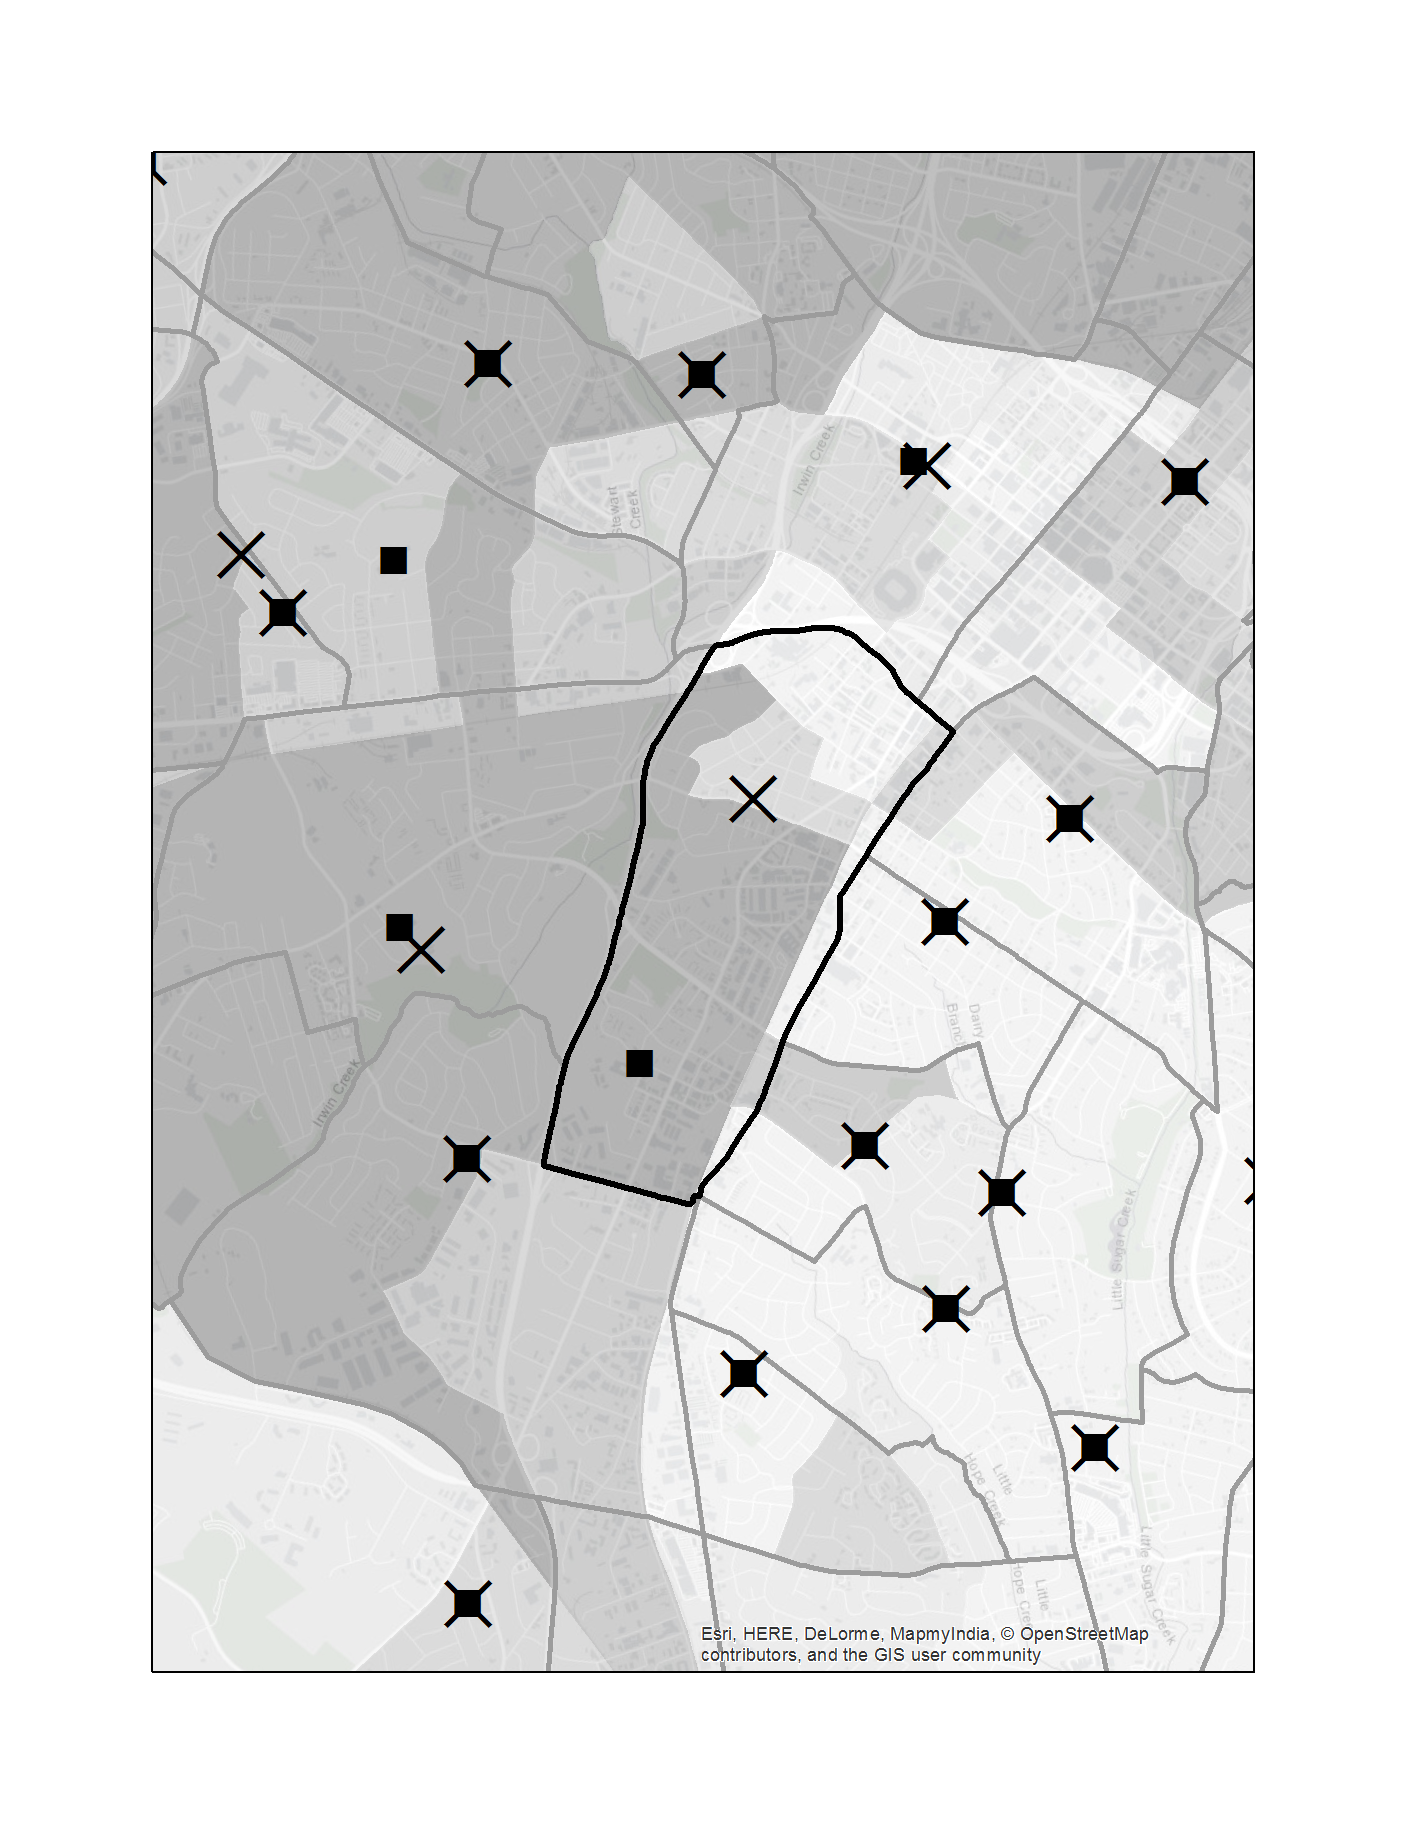
\includegraphics[ width=3.33in,  clip=true,  trim= 1.5in 2.45in 1.5in 2.45in ]{../../50_results_full/Map_Paper_Charlotte_PP_2008_2012.png} \hspace*{.1in}
				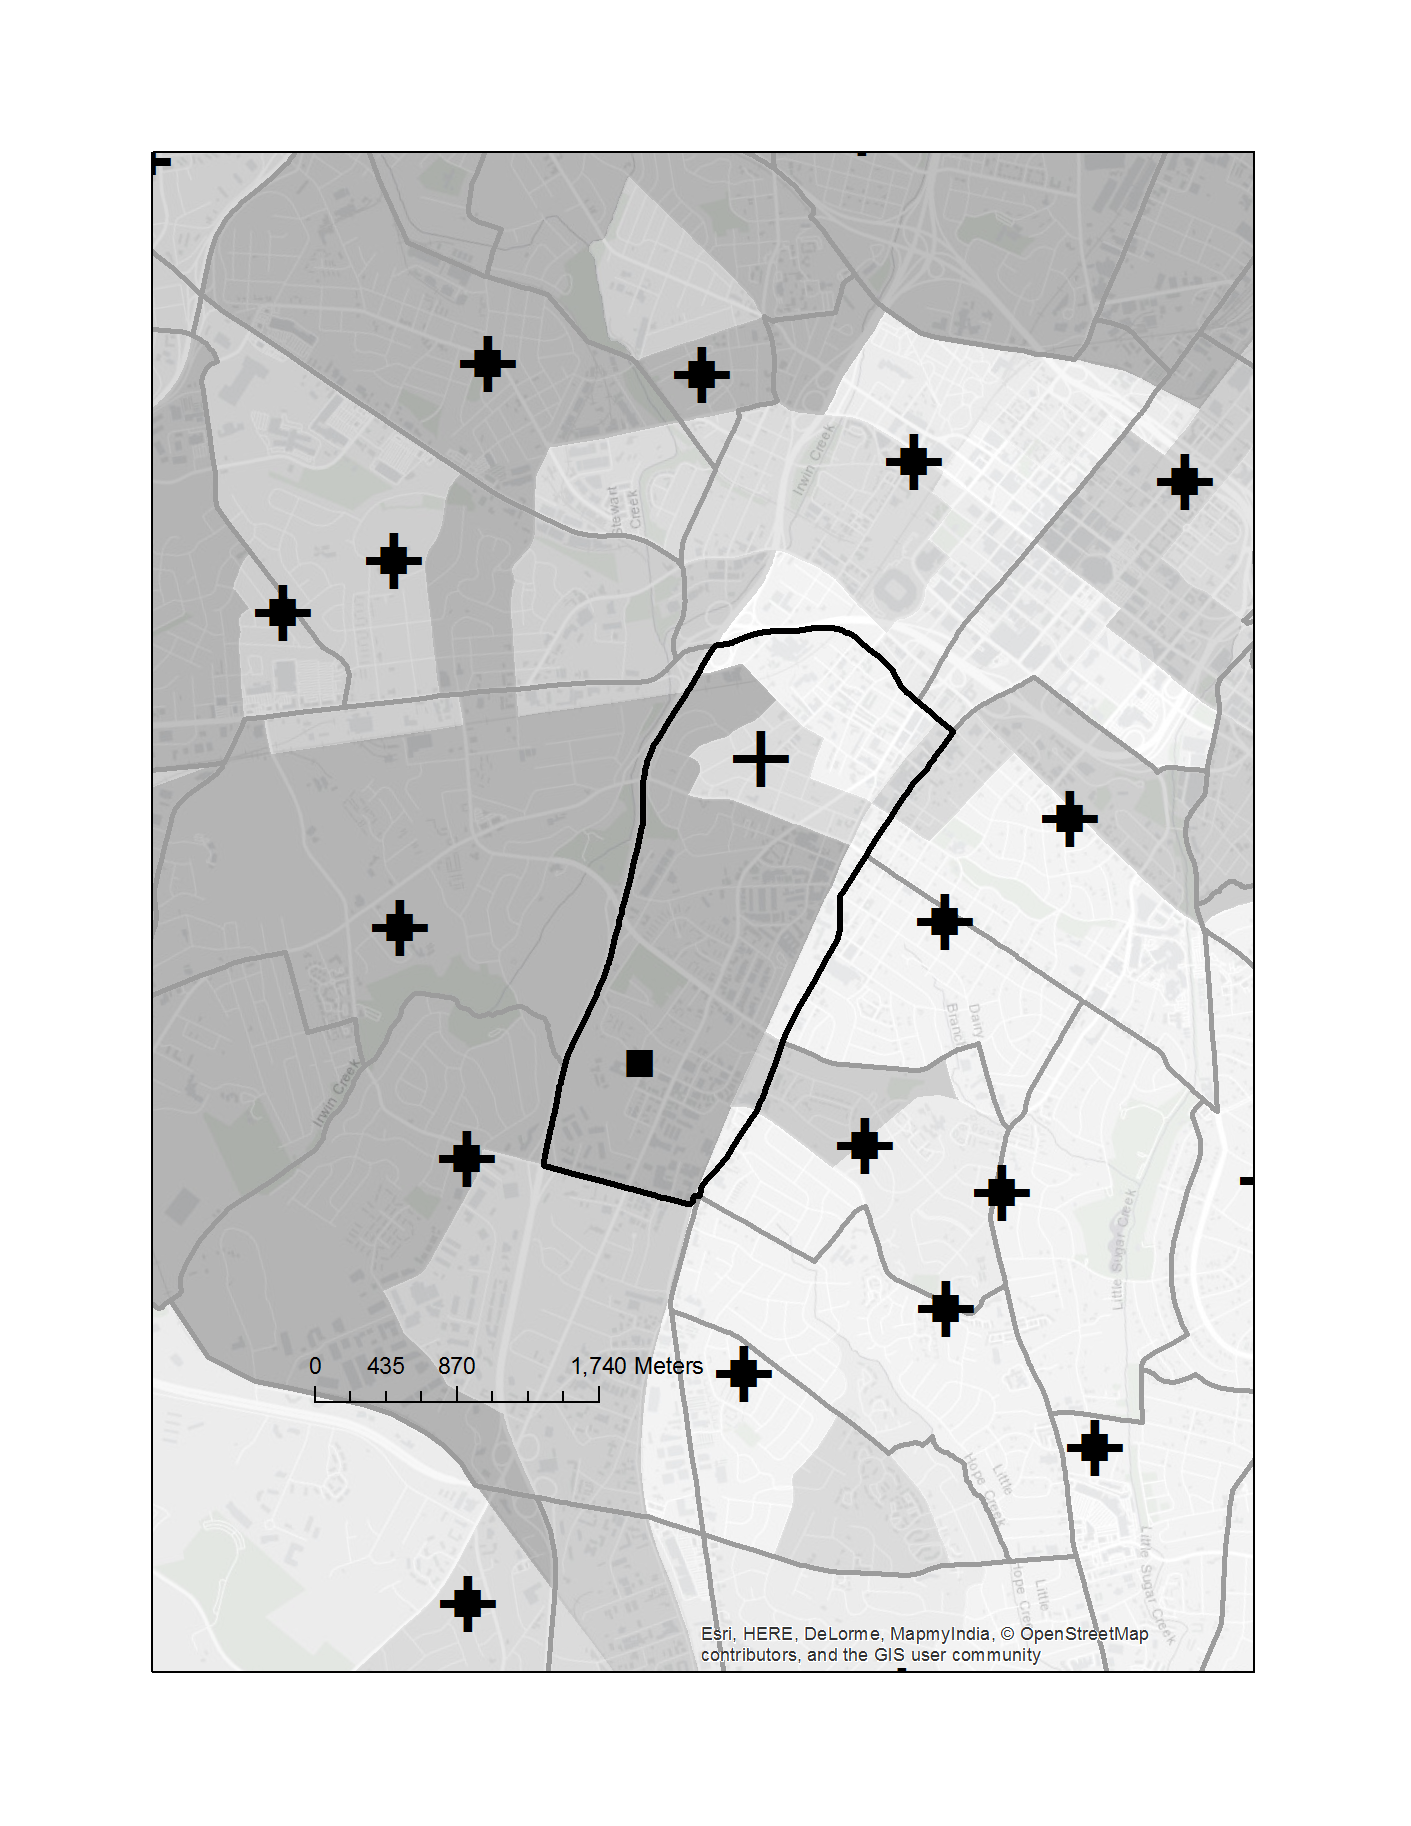
\includegraphics[ width=3.33in,  clip=true,  trim= 1.5in 2.45in 1.5in 2.45in ]{../../50_results_full/Map_Paper_Charlotte_PP_2012_2016.png} \\

				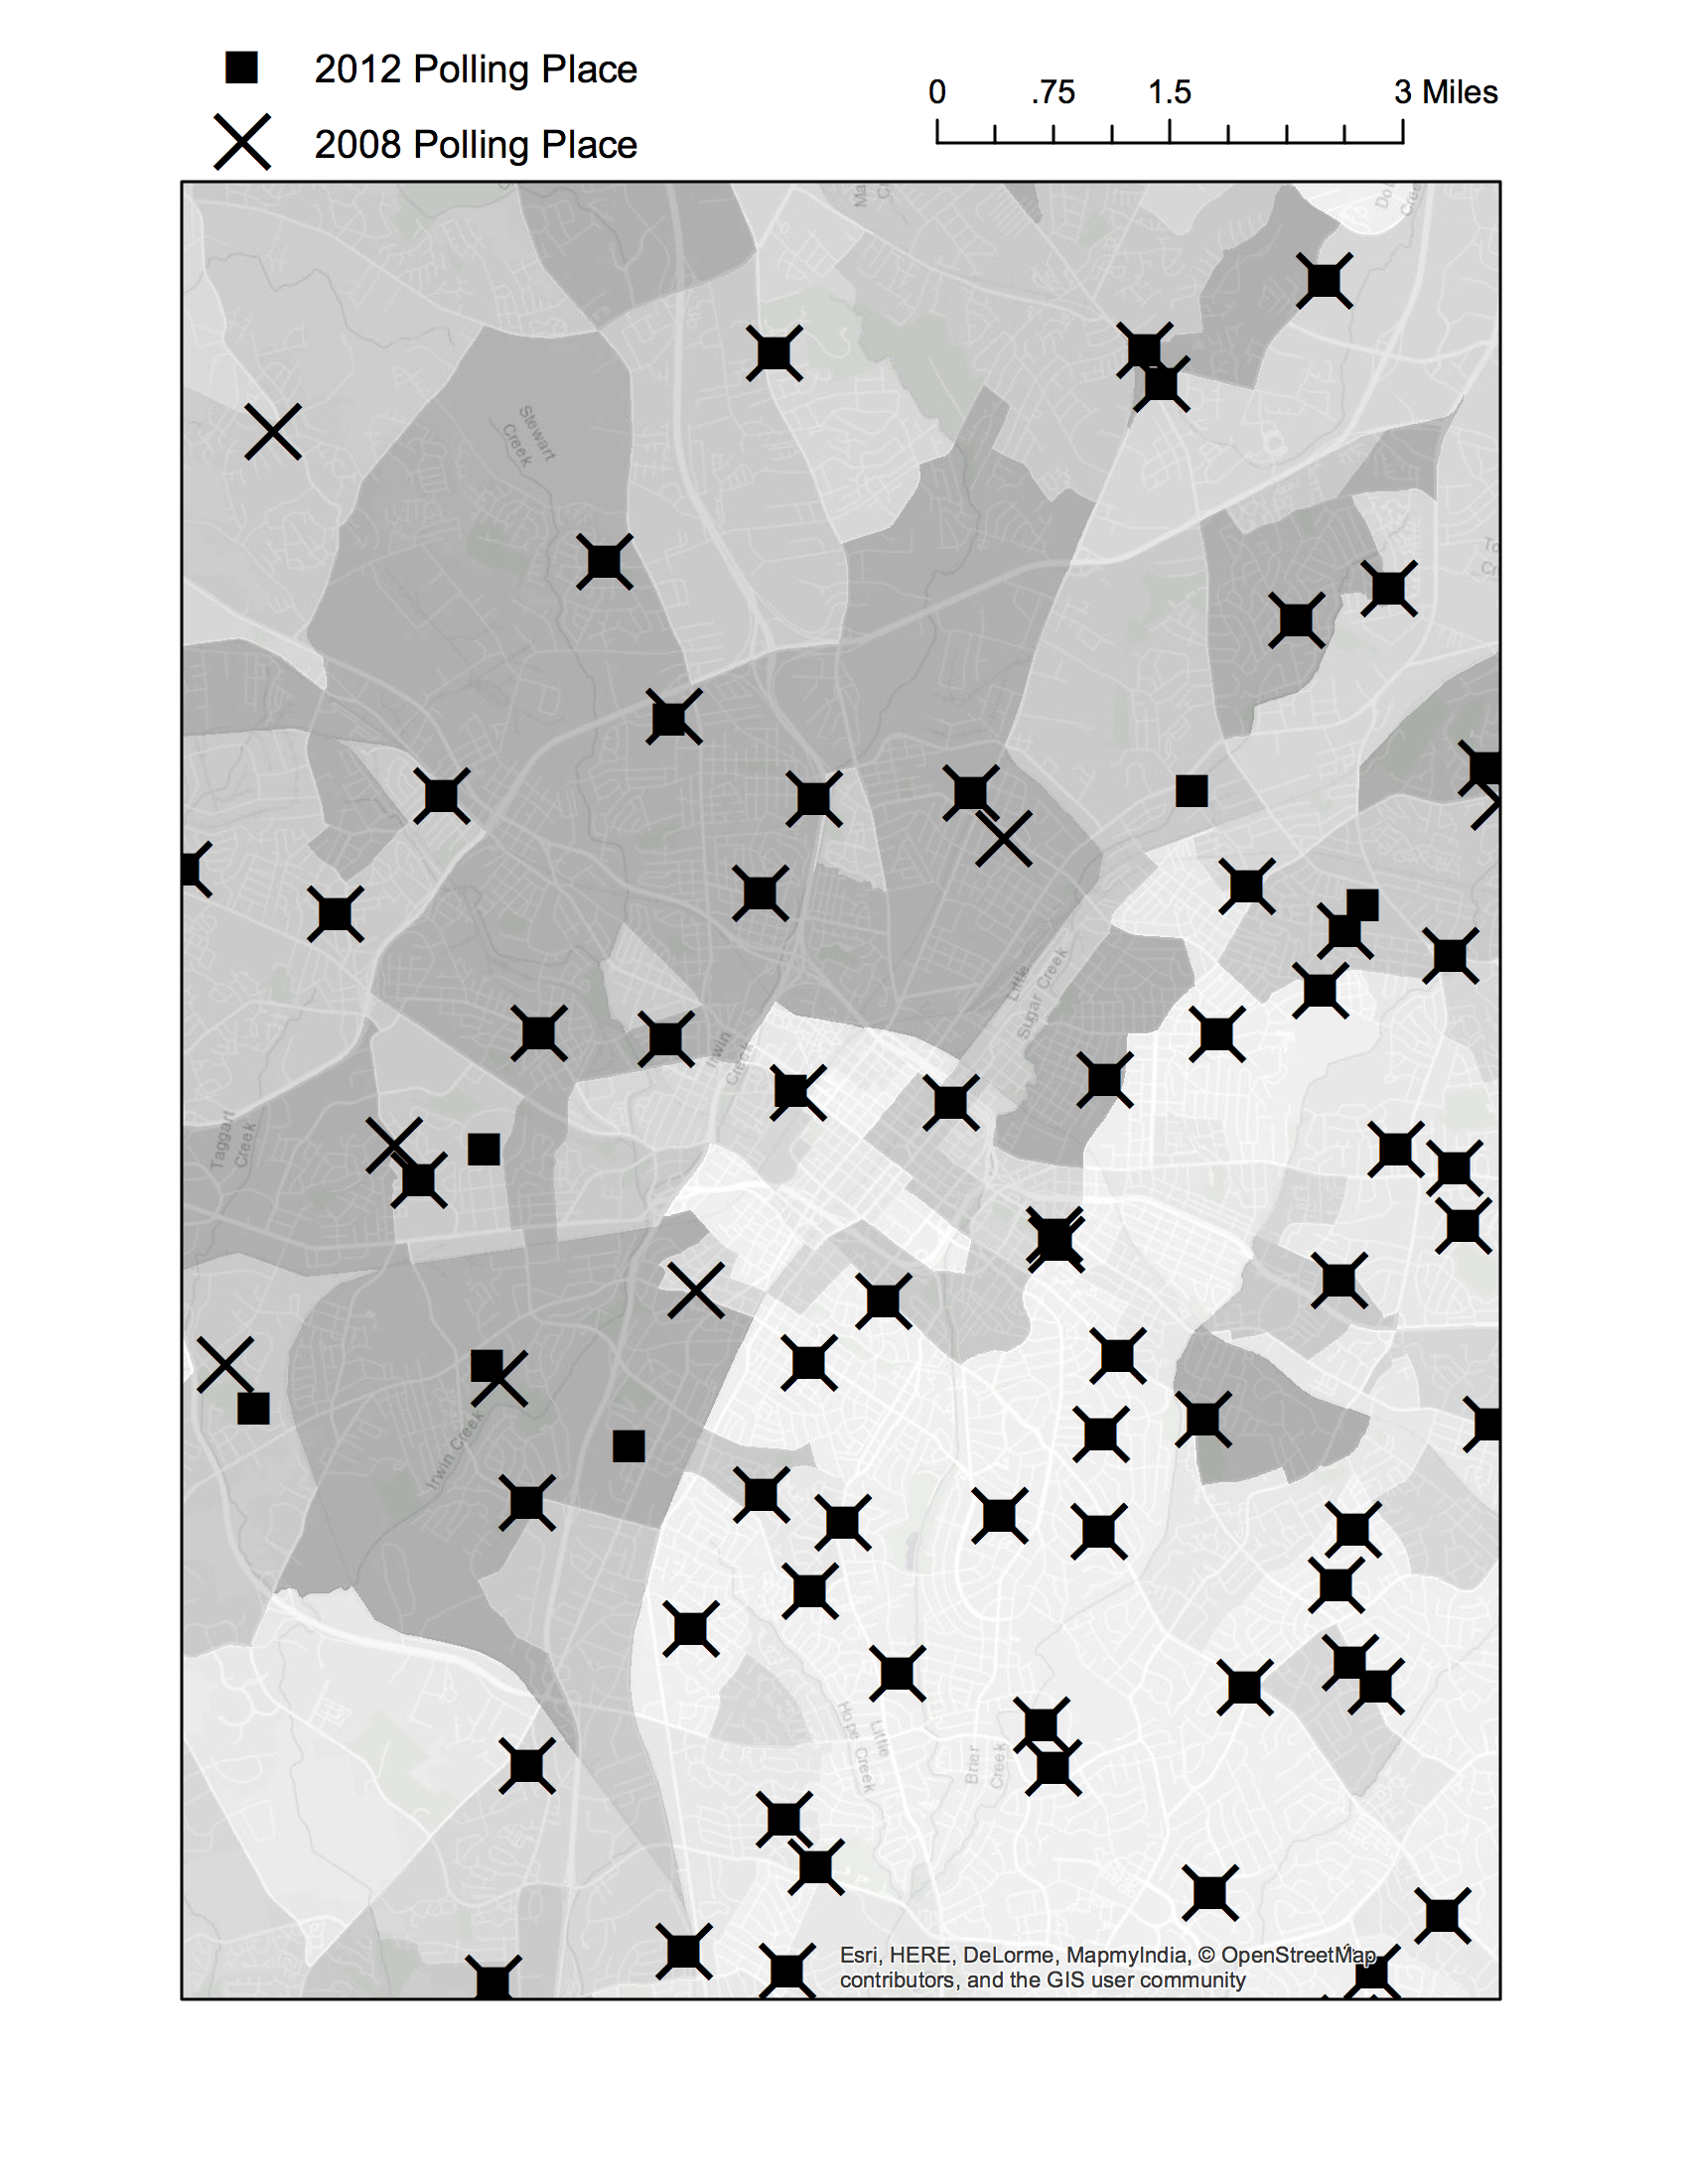
\includegraphics[ width=1.3in,  clip=true,  trim= 1.0in 10.13in 4.9in 0.5in ]{../../50_results_full/Map_Charlotte_PP_Legend_B.png}
				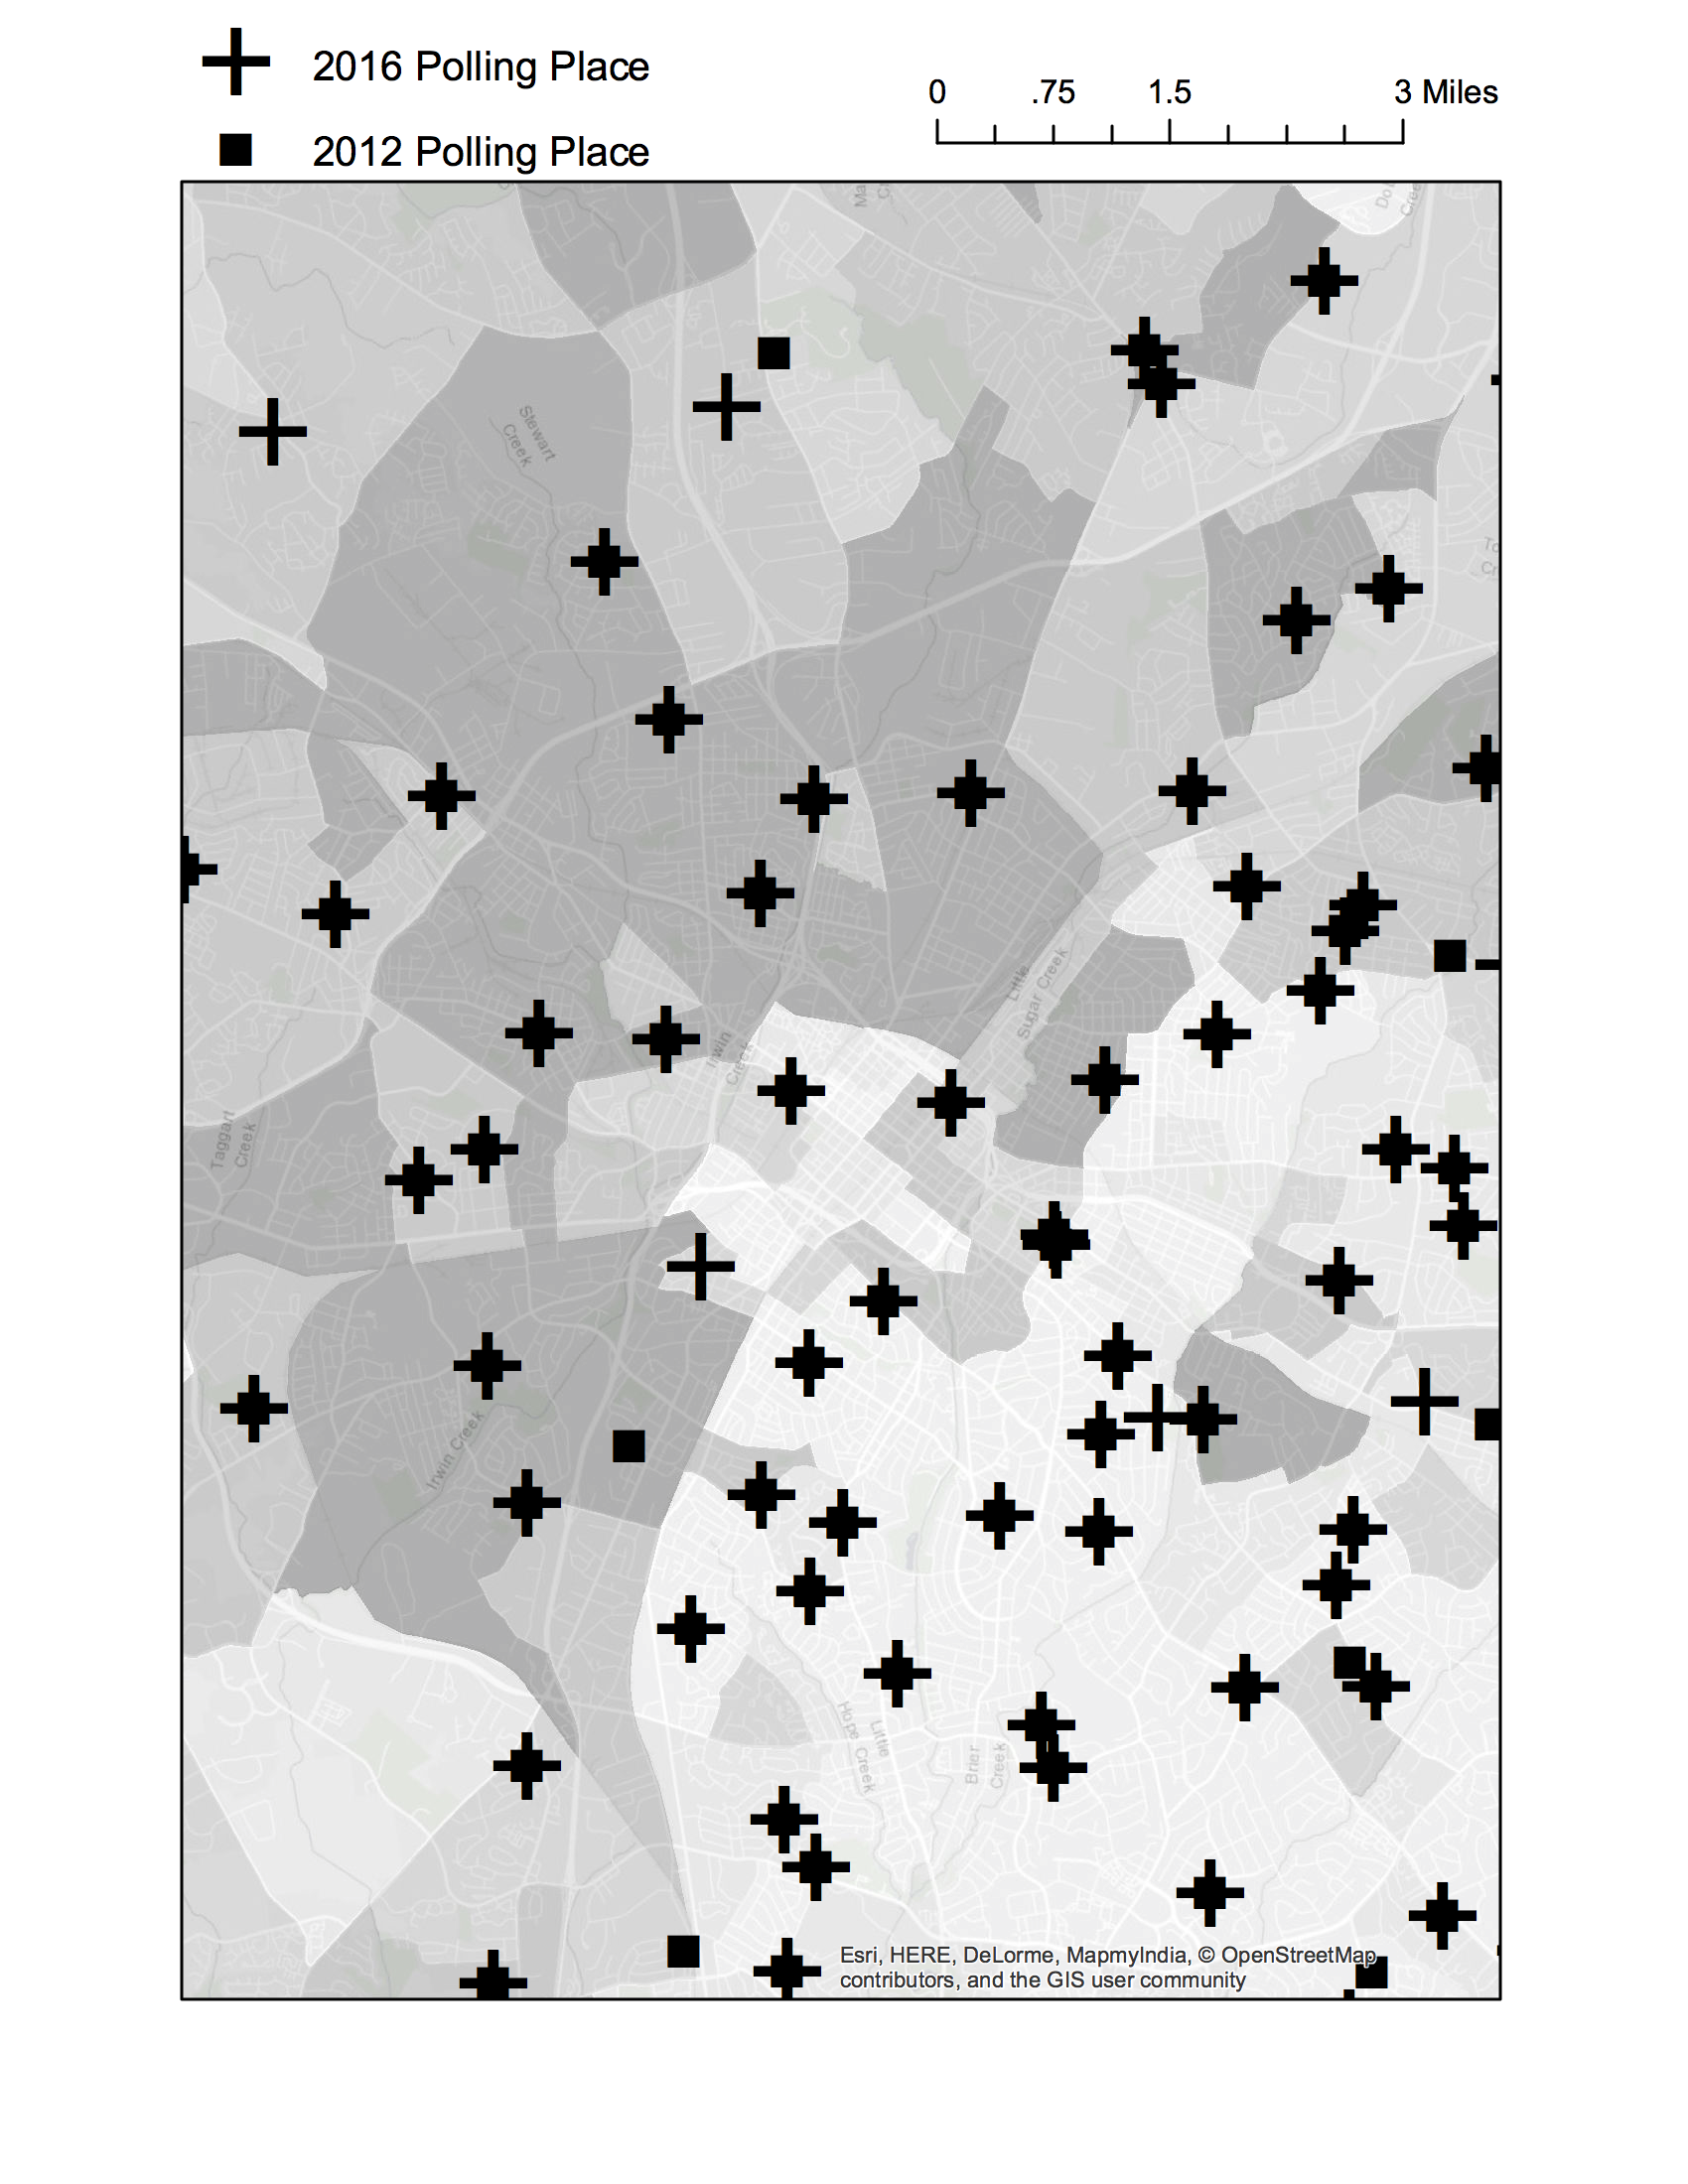
\includegraphics[ width=1.3in,  clip=true,  trim= 1.0in 10.13in 4.9in 0.5in ]{../../50_results_full/Map_Charlotte_PP_Legend_A.png}
				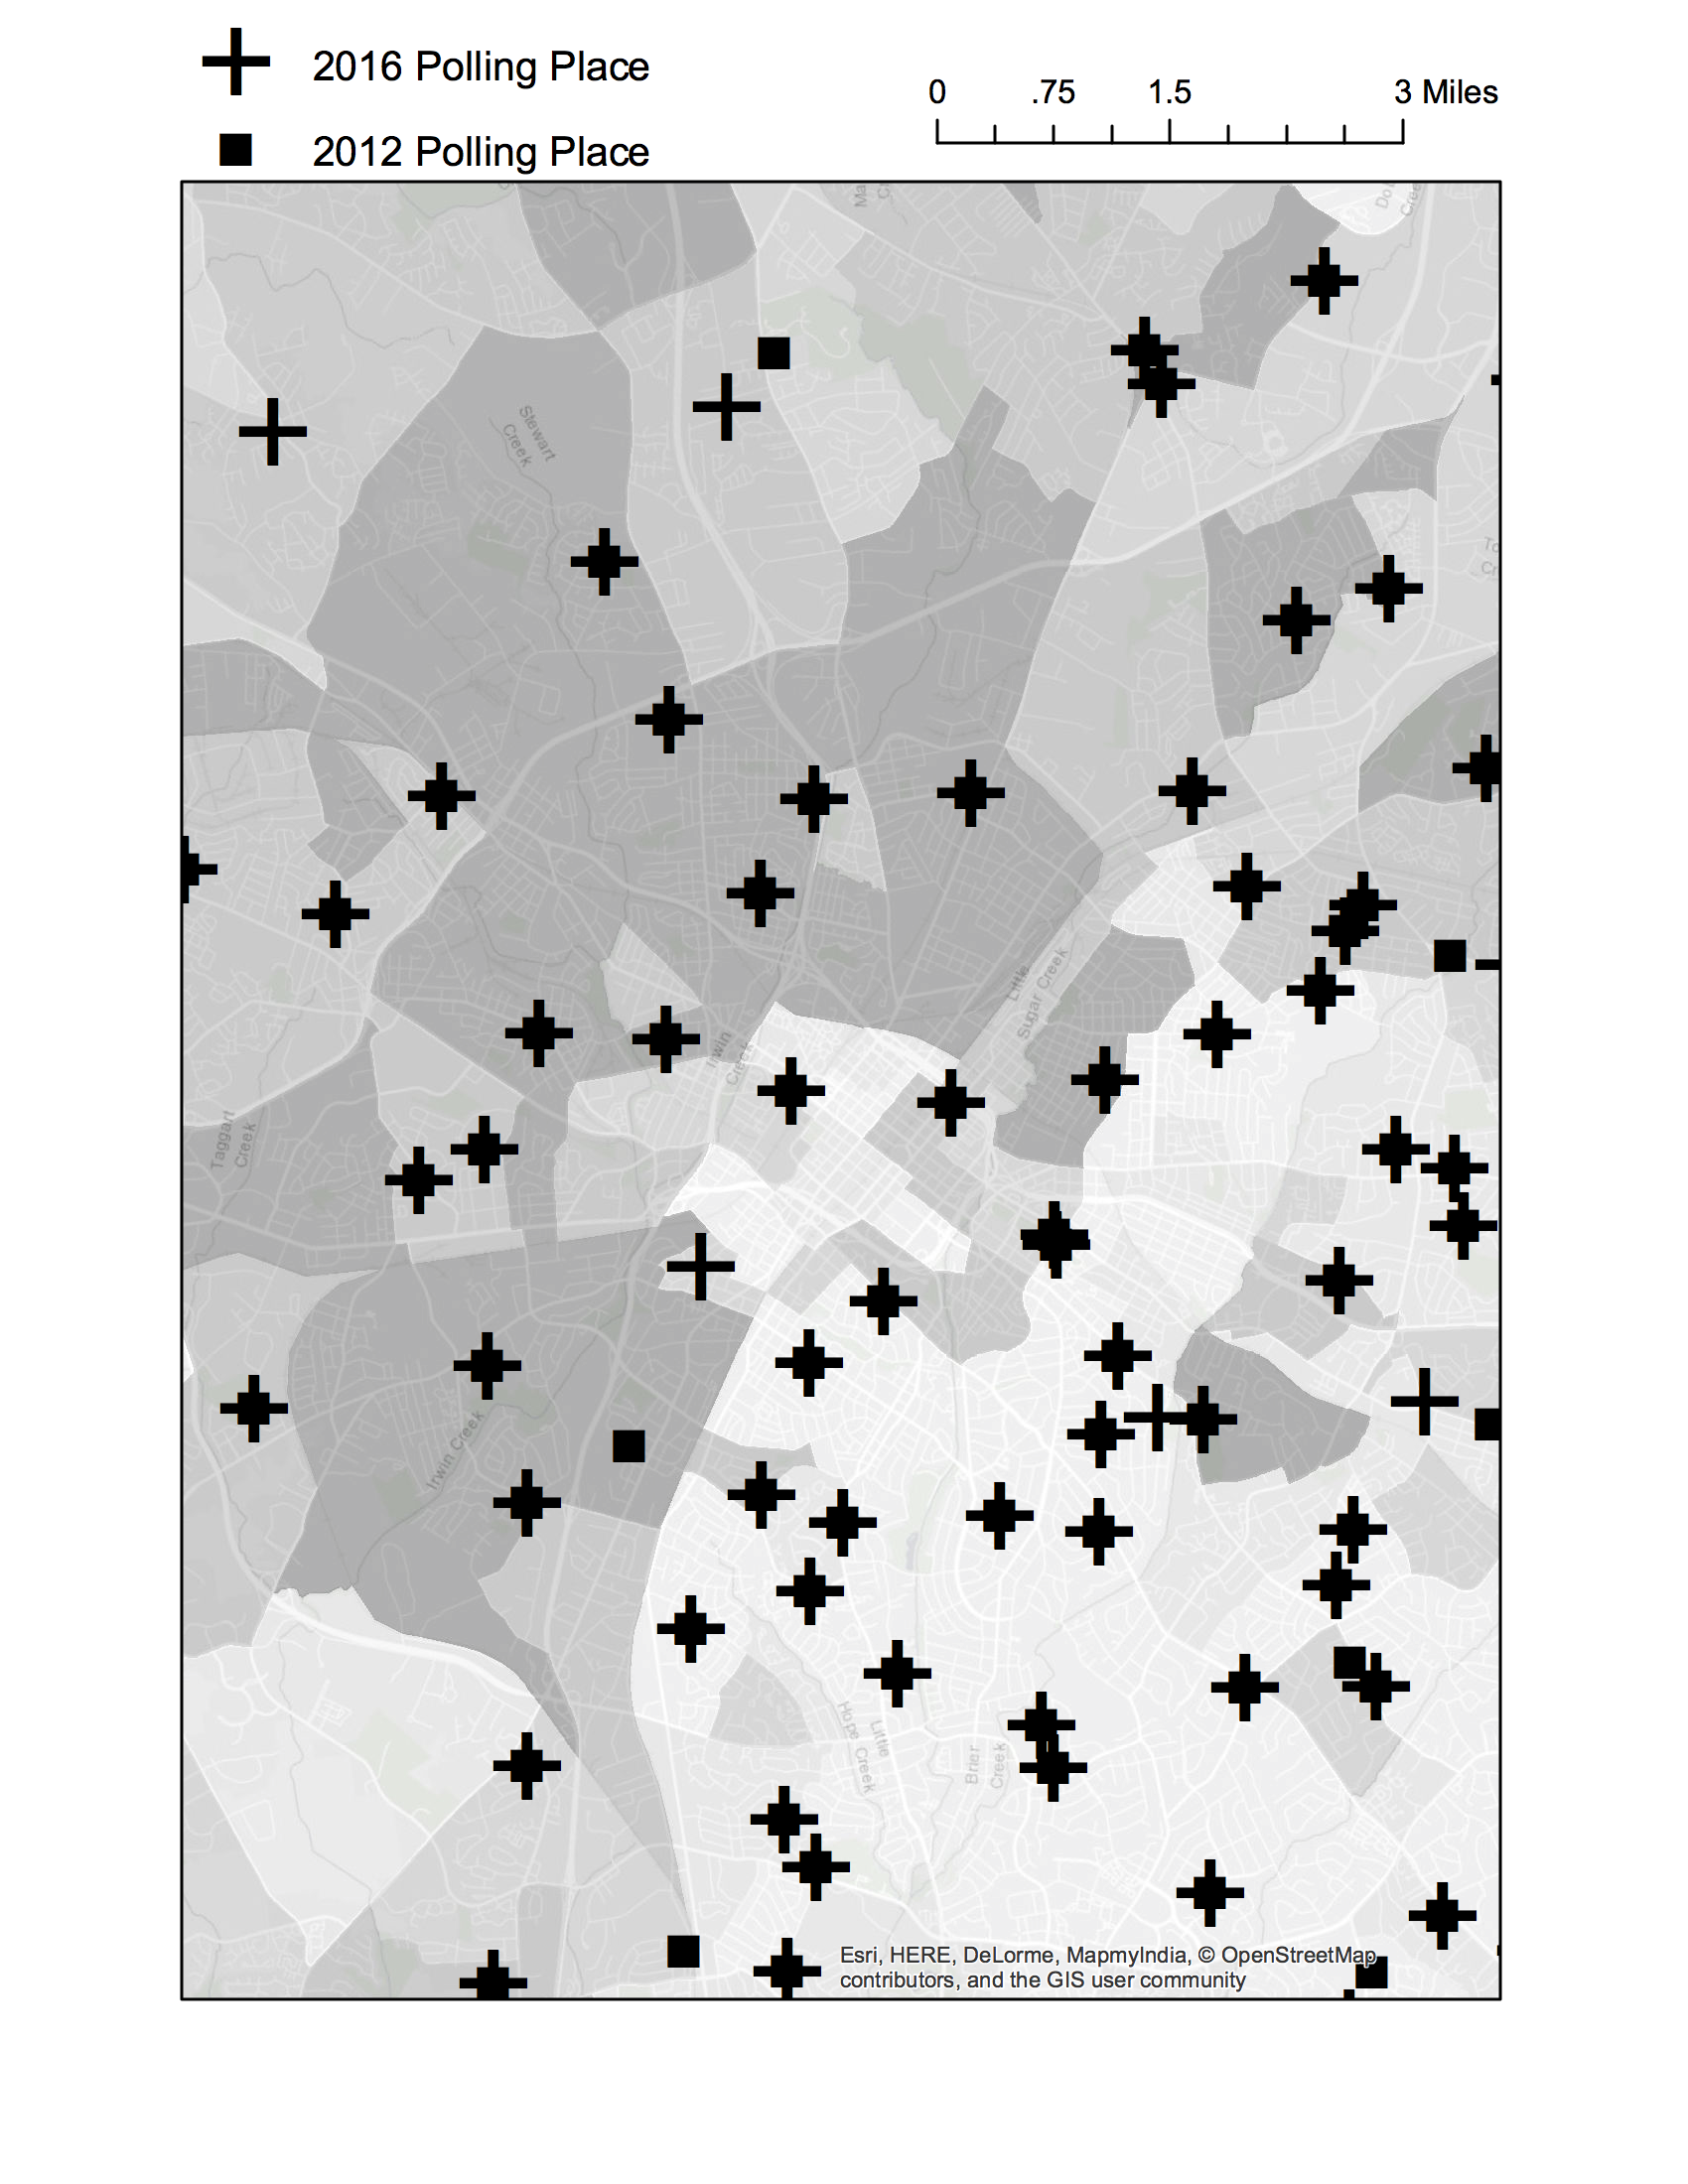
\includegraphics[ width=1.3in,  clip=true,  trim= 1.0in 10.55in 4.9in 0in ]{../../50_results_full/Map_Charlotte_PP_Legend_A.png}
		\vspace*{.05in}
		\label{figure_map_charlotte_pp}
		\end{center}
	\scriptsize{\emph{Notes:}   The above maps illustrate movement in polling place locations using the example of central Charlotte in Mecklenburg county.  Map (a) presents the locations of polling places in 2008 (Xs) and 2012 (squares). Map (b) presents the locations of polling places in 2012 (squares) and 2016 (crosses).  The background is shaded according to the racial composition of census block groups in the 2010 census with darker shades of gray indicating a higher percentage of black residents.  Gray boundaries indicate 2016 precinct boundaries with precinct \#22's boundary outlined in bold black.}
\end{figure} \normalsize


The changes depicted in Figure~\ref{figure_map_charlotte_pp} are the changes we would expect if election administrators were engaged in racial or partisan targeting when deciding where to locate polling places.  However, observing only individual isolated instances of changes such as this, it's difficult to infer intentional manipulation as compared to genuine need.  And even in the case where knowledge of intent were available, it's difficult to know the full extent of manipulation, particularly at higher geographic levels where electoral consequences might obtain---i.e. cities, counties, and the state.  Rather than focus on individual instances, therefore, we examine the state-wide pattern of changes under the assumption that homogeneity in the partisan motivations across all local election boards would be more likely to result in pervasive (rather than one-off) changes, should they occur at all.

TABLE: Who is impacted by changes
%---------------------------------

\begin{table}[t!]\centering \small
\caption{Voters Impacted by Polling Place Changes by Period}\label{table_ppchange}
\vspace*{.055in}
\begin{tabular}{@{\extracolsep{5pt}}l*{4}{c}}
\hline\hline\noalign{\smallskip}
	& \multicolumn{2}{c}{2008-2012} & \multicolumn{2}{c}{2012-2016} \\
	\cline{2-3} \cline{4-5}   \noalign{\smallskip}
	& \# Impacted & Percentage of Group & \# Impacted &  Percentage of Group \\
	\hline \noalign{\smallskip}
	 Registered voters  &      386,896 &   16.53\unskip\% &      368,109 &   15.73\unskip\%  \\
	 Black voters &       78,153 &   17.02\unskip\% &       68,303 &    14.87\unskip\% \\
	 White voters  &      292,030 &   16.39\unskip\% &      285,443 &   16.02\unskip\%  \\
	 Democratic voters  &      178,945 &   16.88\unskip\% &      156,613 &   15.31\unskip\% \\
	 Republican voters &      129,080 &    16.01\unskip\% &      133,285 &    16.44\unskip\% \\
	 Unaffiliated voters &       78,539 &   16.62\unskip\% &       77,836 &  15.41\unskip\%  \\
	\noalign{\smallskip}\hline\hline\noalign{\smallskip}
	\multicolumn{5}{p{6.5in}}{\scriptsize{\emph{Notes:} Absolute number and share of each demographic group impacted by a polling place change in each of the two periods of our analysis. Calculations are based on the sample used in subsequent analyses.  See Section~\ref{section_data} for more details. Percentages are out of total registered voters in a given year. Information on race and party registration are from the official North Carolina Voter rolls and thus refer to voters who are affected, not people more generally.}}
\end{tabular}
\end{table}

Table \ref{table_ppchange} shows the scope of the polling place changes made by Democrats and Republicans occurring within our balanced panel. The Table summarizes a finding that we confirm using more rigorous statistical analyses below: contrary to what we would expect if election administrators were targeting voters from specific parties, polling place changes impact voters of all types at nearly identical rates. In fact, Democrat-led changes were actually slightly more likely to impact Black voters and registered Democrats, whereas Republican-led changes were slightly more likely to impact registered Republican voters. The table shows very little evidence that Democrat-led changes differed from Republican-led changes in either magnitude or who was impacted. Of course, this still leaves open the possibility that the \emph{nature} of polling place changes vary across voters (e.g. administrators may move polling places towards their supporters and away from opposition voters), but as we will show in subsequent analyses, we do not find evidence that this is the case.



%------------------------------------------NORTH CAROLINA --------------------------------------------------%

\section{\large Characterizing Statewide Polling Place Changes in North Carolina}\label{section_nc}
\vspace*{-0.5cm}

We begin by analyzing whether voters are more or less likely to be impacted by precinct and polling place changes depending on their partisanship and race.  To do so, we focus on whether voters from the party \emph{not} in control of election administration---Republican voters in 2012 and Democratic voters in 2016---are (a) more likely to experience polling place changes, (b) more likely to have polling places moved farther from their residence, and (c) more likely to have more voters assigned to their polling place. In addition to estimating the average effect using our full 2008-2016 panel, we also estimate the separate effects for each partisan regime to determine if Republicans or Democrats are more or less likely to target opposition voters.

% The descriptive results in Table \ref{table_ppchange} do not indicate that either Democratic or Republican local election officials allocated polling places in a manner consistent with strategic partisan intent.  However, those descriptive statistics may mask across-county heterogeneity.  We therefore leverage \emph{within}-county variation in polling place changes for every county in North Carolina across three presidential elections.  Because we use a balanced panel of voters, our estimated effects are critically \textit{not} a function of changes in the composition of the electorate between presidential election years.  Moreover, because we remove voters who move residences from our panel, we know that the polling place changes that we observe are due to the actions of election administrators, not the choice of voters to move.

For each investigation, we estimate a variant of the the following linear probability model:\footnote{We use a linear probability model rather than a logit or probit for ease of interpretation and also because the inclusion of fixed effects means that the logit and probit estimates are inconsistent because of the incidental parameters problem for non-linear models.}
\begin{align}
	Pr(\Delta Polling Place_{i,t,c}) = \alpha_{c} + \gamma_{t} + \alpha_{c}\times\gamma_{t} + \beta_1 Opposition_{i,t} + \beta_2 Unaffiliated_{i,t} \nonumber \\
  + \beta_{4}Age_{i,t} + \beta_{5}Age_{i,t}^{2} + \epsilon_{i,t} \label{equation_panel_party}
\end{align}\normalsize

applied to our full panel, as well as separately for 2012 (when changes were made by Democrats) and 2016 (when changes were made by Republicans). $\Delta  Polling Place_{i,t,c}$ is an indicator variable for whether voter $i$ in county $c$ in presidential election year $t$ experienced a polling place change from the previous presidential election; $\alpha_{c}$ captures county fixed effects; $\gamma_{t}$ captures year fixed effects (for the pooled analysis); $\alpha_{c}\times\gamma_{t}$ is an interaction between county and year fixed effects (for the pooled analysis) to account for whether some counties are on different trends in terms of polling place changes.\footnote{We also analyze the dependent variable of voters-per-precinct.  Precincts can be consolidated in such a way as to increase the number of voters that are assigned to a given polling place, potentially increasing wait times.} We also analyze models that rely on \emph{across}-county variation rather than \emph{within}-county variation to look for evidence that differential targeting is a county-level rather than a within-county phenomenon -- i.e., partisan elites target voters of particular groups in only a few counties rather than target precincts of opposition voters statewide.  Our balanced panel of stationary voters further ensures that our results are not a function of changes in the composition of the electorate between elections, nor of voters moving into a precinct or polling place change.  Because polling place changes are made at the county-level, we cluster our standard errors by county.\footnote{Clustering the standard errors by county effectively reduces our (cross-sectional) sample size to 100 counties.  However, as this is the geographic aggregation at which political decisions are made, we think this conservative strategy makes sense.  We pay particular attention to the magnitude of our effects, recognizing that this clustering strategy may be too conservative.}

To identify whether Democrats target Republican voters with polling place changes and vice versa for Republicans, we indicate whether voter $i$ is member of the opposing party of the Governor and consequently the partisan-appointed county election board ($Opposition$).\footnote{Note that while claims of manipulation have been leveled at the local county board of elections, who have the closest knowledge of their counties and precincts, our empirical approach is actually agnostic about whether it is the county boards, state boards or governor who is responsible for targeting, were it to occur.} Given the change in partisan control, $Opposition$ takes a value of 1 for Republican voters in 2012 when Democrats were in charge (0 for Democrats), and a value of 1 for Democrat voters in 2016 when Republicans were in charge (0 for Republicans).  We also control for linear and quadratic age.\footnote{Age might be related to geographic clusters of renting or homeownership which could conceivably be related to some geographic patterns of genuine need for polling place changes.  Some news reports have contended that young voters have sometimes been targeted with early voting polling place changes \citep{roth2015x}.}

To examine the separate effects of race we augment specification \ref{equation_panel_party} using:
\begin{align}
   Pr(\Delta Polling Place_{i,t,c}) = \alpha_{c} + \gamma_{t} +  \alpha_{c}\times\gamma_{t}    \nonumber \\
    + \beta_1 WhiteOpposition_{i,t}  + \beta_2 BlackOpposition_{i,t} + \beta_3 OtherOpposition_{i,t}   \nonumber \\
  + \beta_4 WhiteUnaffiliated_{i,t}   + \beta_5 OtherUnaffiliated + \beta_{4}Age_{i,t} + \beta_{5}Age_{i,t}^{2}  + \epsilon_{i,t}. \label{equation_panel_partyrace}
\end{align}\normalsize

The coefficients of interest on each of our indicator variables in equation~\ref{equation_panel_partyrace} reflect the average probability a voter of that demographic or social group experiencing a polling place change relative to the base category, a co-partisan of the Governor (and therefore local election administrators) \emph{of any race}.\footnote{For ease of exposition, Libertarians have been dropped (only          0.1\unskip\% of voters are Libertarian).} We do not estimate the coefficients on base categories for each race (which would capture the differential effects of a race for a \emph{co-partisan} of the governor) because we don't have theoretical priors about how or why administrators would differentially change the polling places of their own supporters differently because of their race.  Statistically significant and/or substantively large coefficients for voters of a particular race or partisanship provides evidence consistent with possible strategic targeting for electoral gain because they indicate that the group of voters is more likely to be affected by a polling place change than voters associated with the party in control of election administration.

Of course, strategic partisan targeting is not the only reason that polling places might be moved.  There may sometimes be a genuine technocratic need to move a polling place---e.g. for reasons of cost, disability access, parking or other relatively mundane non-strategic reasons.  Were it the case that the incidence of genuine need were related to the partisanship or race of voters within a given precinct, then our estimates of targeting would be confounded.  However, we have no evidence to suggest that such a correlation between factors of genuine need and the partisanship and race of nearby voters exists.  Furthermore, and even more compellingly, we have no reason to think that the genuine need to move a polling place is related to the \emph{opposition status} of voters, and thus, which party is in charge of making changes.  We do not expect greater need in Democratic areas when Republicans are in charge nor greater need in Republican areas when Democrats are in charge. We therefore do not expect that the genuine need for change confounds our estimation of partisan targeting.

Table \ref{table_pp_panel} begins by presenting the estimated effects of a voter's partisanship and race on the likelihood that they experience a polling place change. Models 1-5 present the results for party only using equation~\ref{equation_panel_party}; models 6-8 estimate equation~\ref{equation_panel_partyrace} examining differential changes by both party and race.   Columns 1, 2, 3 and 5 present the results for the full panel and provide a sense of the overall likelihood of a non-co-partisan or non-white voter being affected by a change regardless of the party in control.\footnote{Caution should be used in interpreting the \emph{Black Opposition} category in column 6, as the population of Black Republicans is extremely small in North Carolina (        96.6\unskip\% of Republicans identify as White).}

%% TABLE: Main Targeting Table
%%----------------------------
\begin{table}[t!]\centering \footnotesize
\def\sym#1{\ifmmode^{#1}\else\(^{#1}\)\fi}
	\caption{The Probability of Experiencing a Polling Place Change}\label{table_pp_panel}
	\smallskip
	\begin{tabular}{@{\extracolsep{5pt}}l*{8}{c}}
	\noalign{\smallskip}\hline\hline\noalign{\smallskip}\noalign{\smallskip}
			&  \multicolumn{7}{c}{$Pr(\Delta Polling Place)$}   \\
			\cline{2-9}  \noalign{\smallskip}
                            &\multicolumn{1}{c}{(1)}         &\multicolumn{1}{c}{(2)}         &\multicolumn{1}{c}{(3)}         &\multicolumn{1}{c}{(4)}         &\multicolumn{1}{c}{(5)}         &\multicolumn{1}{c}{(6)}         &\multicolumn{1}{c}{(7)}         &\multicolumn{1}{c}{(8)}         \\
\midrule
\emph{Opposition}&  -0.0083         &   0.0030         &   0.0028         &   0.0031         &   0.0020         &                  &                  &                  \\
                & (0.0055)         & (0.0021)         & (0.0025)         & (0.0047)         & (0.0046)         &                  &                  &                  \\
\emph{WhiteOpposition}&                  &                  &                  &                  &                  &   0.0016         &   0.0033         & -0.00035         \\
                &                  &                  &                  &                  &                  & (0.0023)         & (0.0050)         & (0.0030)         \\
\emph{BlackOpposition}&                  &                  &                  &                  &                  &   0.0061         &   0.0012         &   0.0054         \\
                &                  &                  &                  &                  &                  & (0.0092)         & (0.0063)         &  (0.010)         \\
\midrule
County FE       &                  &\checkmark         &\checkmark         &\checkmark         &\checkmark         &\checkmark         &\checkmark         &\checkmark         \\
Year FE         &                  &\checkmark         &\checkmark         &                  &                  &\checkmark         &                  &                  \\
Ct. x Yr. FE    &                  &\checkmark         &\checkmark         &                  &                  &\checkmark         &                  &                  \\
Controls        &                  &                  &\checkmark         &\checkmark         &\checkmark         &\checkmark         &\checkmark         &\checkmark         \\
Year Sample     &    Panel         &    Panel         &    Panel         &     2012         &     2016         &    Panel         &     2012         &     2016         \\
Observations    &  4677529         &  4677529         &  4677529         &  2338992         &  2338537         &  4677529         &  2338992         &  2338537         \\
Mean of DV      &     0.16         &     0.16         &     0.16         &     0.17         &     0.16         &     0.16         &     0.17         &     0.16         \\
SD of DV        &     0.37         &     0.36         &     0.36         &     0.35         &     0.34         &     0.36         &     0.35         &     0.34         \\
\\
    \noalign{\vspace*{-.17in}}\hline\hline\noalign{\smallskip}
    \multicolumn{9}{p{6.4in}}{\scriptsize  \emph{Notes:} Coefficients are from estimating Equation~\ref{equation_panel_party} (Columns 1-5) and Equation~\ref{equation_panel_partyrace} (Columns 6-8).  The unit of analysis is the voter-election in the panel models and the voter in the cross-sectional models.  In all models, the reference (excluded) category is a voter of the same party as the Governor. Appendix~\ref{appendix_maintargeting} reports coefficient estimates including those for unaffiliated voters.  The SD of the DV is the average of the within-$i$ standard deviations of the outcome variable for the full panel. Standard errors clustered at the county level. \sym{*} \(p<0.1\), \sym{**} \(p<0.05\), \sym{***} \(p<0.01\) }
\end{tabular}
\end{table}

Across our models, we see no evidence that voters of the opposition party nor Black voters are more likely to be impacted by polling place changes, \emph{on average} across all voters and, thus, all counties in the state.  Column 1 reports the basic panel correlation of the average probability of an opposition voter being targeted statewide across the time period absent controls.  If widespread targeting occurred only in specific \emph{counties} ---for instance, in counties with a large number of opposition voters---this specification would detect changes affecting opposition voters within those \emph{particular} counties.  The resulting naive correlation in Column 1 is substantively small (about 1 percentage point) and statistically indistinguishable from zero.  Including fixed effects and controls (models 2, 3 and 5) fails to change the substantive conclusion.  Opposition voters appear to be \emph{slightly} more likely to experience polling places changes under both partisan regimes on average, but the magnitude of the effect is statistically and substantively insignificant ---non-copartisans of the election board majority are less than a quarter of one percentage point more likely to experience a polling place change than a co-partisan of the board's majority party.

To determine whether these effects vary between Democrats and Republicans, we use the same specification (absent year fixed effects) to estimate the effects separately for each partisan regime. This analysis is motivated by the fact that most media coverage of polling place changes in North Carolina has suggested that such changes are primarily a strategy used by Republicans. Decomposing the pooled estimates of models (1, 2, 3, and 5) by party reveals similar near-zero effects.  Model 4 shows that under Democratic control in 2012, Republican voters appear to be roughly a third of a percentage point more likely to experience a polling place change overall. Model 5 shows that under Republican control in 2016, opposition voters were even less likely to experience polling place changes---Democratic voters were only approximately 0.2 percentage points more likely than Republican voters to experience a change.\footnote{Although we focus on the substantive magnitude of that effect given what we've previously noted about our conservative standard error clustering choice, we note that the effect would have to about 0.5 percentage points (an estimated coefficient of 0.0049 approximately) for us to reject the null hypothesis that the point estimate is zero.}

Allowing the probability of experiencing a polling place change to vary by both partisanship and race for the full panel (Model 6), for Democrat control (Model 7) and for Republican control (Model 8) reveals a similar lack of effects consistent with intentional targeting. Despite widespread journalistic accounts to the contrary, the results fail to detect dramatic differences in the probability of experiencing a polling place change by race when Republicans were in control.  Black Democrats are more likely than white Democrats to experience a change in Model 8, but the effect is only about half of one percentage point and statistically indistinguishable from zero.

In concluding that there is no evidence of strategic targeting of polling place changes for partisan gain on average, we emphasize the small magnitudes we detect---less than half of one percentage point in all relevant cases.  Although our county-level clustering limits the precision of our estimates, even if we were somehow able to increase our statistical power and reject the null hypothesis that these effects were exactly zero, the magnitudes would remain substantively minuscule; the estimated effects amount to just 2\% of one standard deviation of the outcome.

In addition to determining whether opposition voters are more likely to experience a polling place change, it is also important to determine the type of change they experience.  While polling place changes are generally seen as raising costs to voters, it seems plausible that election administrators could believe that reducing travel times may have a \emph{net} positive effect on turnout by making it easier to vote. If so, the lack of effect in \ref{table_pp_panel} could reflect the fact that although both co-partisan and opposition voters were equally impacted by polling place changes, the changes moved polling place changes closer to co-partisan voters and further from opposition party voters.

Table~\ref{table_pp_panel} evaluates whether our previous results are hiding important variation in \emph{where} polling places are moved relative to voters of a particular party or race.  We estimate the relationship between voter partisanship, race and the probability of having a polling place \emph{moved further away} using the set of voters who experience a polling place change.  To do so, we re-estimate specifications (equation~\ref{equation_panel_party} and equation~\ref{equation_panel_partyrace}) with the inclusion of an indicator, $PollingPlaceMovedFurther$, for whether the voter had their polling place moved further away (as measured by drive time) relative to the last presidential election.  (Using more precise measures based on the change in drive time produces similar estimates.) The excluded category is having a polling place moved closer.

%% TABLE: PP FARTHER AWAY
%%------------------------
\begin{table}[t!]\centering \footnotesize
\def\sym#1{\ifmmode^{#1}\else\(^{#1}\)\fi}
	\caption{The Probability of Experiencing a Polling Place Change Moved Farther}\label{table_farther_panel}
	\smallskip
	\begin{tabular}{@{\extracolsep{5pt}}l*{8}{c}}
	\noalign{\smallskip}\hline\hline\noalign{\smallskip}\noalign{\smallskip}
			&  \multicolumn{7}{c}{$Pr(Polling Place Moved Farther)$}   \\
			\cline{2-9}  \noalign{\smallskip}
				                &\multicolumn{1}{c}{(1)}         &\multicolumn{1}{c}{(2)}         &\multicolumn{1}{c}{(3)}         &\multicolumn{1}{c}{(4)}         &\multicolumn{1}{c}{(5)}         &\multicolumn{1}{c}{(6)}         &\multicolumn{1}{c}{(7)}         &\multicolumn{1}{c}{(8)}         \\
\midrule
\emph{Opposition}&   0.0036         &   0.0071         &   0.0067         &   0.0066         &   0.0066         &                  &                  &                  \\
                & (0.0094)         & (0.0075)         & (0.0088)         &  (0.011)         &  (0.011)         &                  &                  &                  \\
\emph{WhiteOpposition}&                  &                  &                  &                  &                  &   0.0043         &   0.0062         &   0.0047         \\
                &                  &                  &                  &                  &                  & (0.0052)         &  (0.011)         & (0.0077)         \\
\emph{BlackOpposition}&                  &                  &                  &                  &                  &    0.014         &    0.015         &    0.012         \\
                &                  &                  &                  &                  &                  &  (0.022)         &  (0.014)         &  (0.023)         \\
\midrule
County FE       &                  &\checkmark         &\checkmark         &\checkmark         &\checkmark         &\checkmark         &\checkmark         &\checkmark         \\
Year FE         &                  &\checkmark         &\checkmark         &                  &                  &\checkmark         &                  &                  \\
Ct. x Yr. FE    &                  &\checkmark         &\checkmark         &                  &                  &\checkmark         &                  &                  \\
Controls        &                  &                  &\checkmark         &\checkmark         &\checkmark         &\checkmark         &\checkmark         &\checkmark         \\
Year Sample     &    Panel         &    Panel         &    Panel         &     2012         &     2016         &    Panel         &     2012         &     2016         \\
Observations    &   754298         &   754298         &   754298         &   386564         &   367734         &   754298         &   386564         &   367734         \\
Mean of DV      &     0.55         &     0.55         &     0.55         &     0.53         &     0.57         &     0.55         &     0.53         &     0.57         \\
SD of DV        &     0.50         &     0.48         &     0.48         &     0.47         &     0.47         &     0.48         &     0.47         &     0.47         \\
 \\
	\noalign{\vspace*{-.17in}}\hline\hline\noalign{\smallskip}

\multicolumn{9}{p{6.3in}}{\scriptsize \emph{Notes:}  The table presents coefficients from estimating Equation~\ref{equation_panel_party} (columns 1-4) and Equation~\ref{equation_panel_partyrace} (columns 5-7), conditional on having had a polling place changed.  The excluded category for the outcome is having had a polling place moved closer. The unit of analysis is the voter-election in the panel models, and the voter in the cross-sectional models. Our controls are linear and quadratic $Age$. See Appendix~\ref{appendix_maintargeting} for the full set of coefficient estimates.  The SD of the DV is the average of the within-$i$ standard deviations of the outcome variable for the full panel models.  Standard errors robust to 100 clusters at the county level.  \sym{*} \(p<0.1\), \sym{**} \(p<0.05\), \sym{***} \(p<0.01\)}
\end{tabular}
\end{table}

Table \ref{table_farther_panel} reports the results. In no model is there a meaningful difference in how polling places are moved for opposition voters relative to voters aligned with the party in control.  In every specification---including both cross-sectional and panel models---we estimate extremely small relationships (less than 1.5 percentage points) between partisanship and the change in distance to a polling place.  Moreover, none of the changes are statistically distinguishable from zero.  Because the results of Table \ref{table_farther_panel} condition on voters who experience a polling place change, a point estimate of 0.67 percentage points (model 3) does not imply opposition voters are three-quarters of a percentage point more likely to have their polling place moved away from them than non-opposition voters; rather it says that \emph{among the $\sim 16\%$ of voters who experience a polling place change}, opposition voters are 0.67 percentage points more likely to have their polling place moved away from them. There is no effect for the other 84\% of voters. Consequently, the overall potential electoral implications of these estimates are even smaller than they may initially appear.\footnote{Again, our conservative standard error clustering may make the statistical tests more conservative than usual, but the small point estimates suggest that, on average, election administrators are unlikely to be moving polling places further from opposition voters (or, conversely, closer to their supporters) statewide.} Allowing the effects to vary by race reveals a similar lack of detectable differences -- black Democrats are more likely to have their polling place moved further away relative to white Democrats (model 8), but the estimated difference is very small both substantively (about 1 percentage point) and statistically.\footnote{Given our standard error clustering choice and the use of a 95\% confidence interval, the effect of opposition targeting of moving a polling place further would need to be about 2 percentage points (a point estimate of 0.017) to statistically distinguish it from zero.}

In addition to controlling where polling places are located, local election officials can also change the boundaries of electoral precincts that determine which polling places are used by which voters.\footnote{Our measure of polling place changes already captures changes that are a function of precinct boundary changes---that is, because $\Delta PollingPlace$ is measured at the voter-level, we code a voter as experiencing a polling place change even if that change has occurred because she was assigned to a new precinct.  Thus, measuring a change in precinct alone does not give us additional analytic leverage beyond our measure of polling place change.} Unlike some states, North Carolina does not have a legal maximum precinct size, thus election officials are not constrained in how many voters they can assign to a given polling place.  As a result, officials can increase the cost of voting at a polling place by re-precincting a polling place to serve more voters even without moving the polling place itself. Including more voters in a precinct can increase the likelihood that voters in the precinct would have to wait in longer lines to cast their ballots. To investigate whether partisan election officials re-precinct in a way that increases the number of voters at a given polling place by the race or partisanship of voters.  For the sake of space, Appendix~\ref{appendix_change_voters_per_pp} reports the results of estimating equations~\ref{equation_panel_party} and equation~\ref{equation_panel_partyrace} for the outcome $\Delta VotersPerPrecinct$.\footnote{Note that this measure is at the level of the voter, and that voters may see the number of \emph{other} voters registered at their polling place change even if their own polling place assignment does not (if new voters are assigned to said voter's polling place).}  Consistent with the findings reported above, we find no evidence that voters are differentially impacted by changes in the number of voters per precinct.

%%------------------------------------------- SECTION ----------------------------------------%%

\section{\large Characterizing County-Level Changes}\label{section_countylevelanalysis}
\vspace*{-0.5cm}

Although we do not find evidence that partisan local election administrators moved polling places---either in general, or more specifically, farther away from opposition voters (or, closer to their own supporters)---nor changed precinct boundaries in a manner consistent with strategic manipulation for partisan electoral gain statewide, it is possible that the average null statewide effects masks strategic targeting occurring in particular counties.  To determine whether some counties -- i.e., some election election officials -- engage in targeting we estimate equation~\ref{equation_panel_party} separately for each of the 100 counties in North Carolina under each partisan regime to determine the probability of each type of voter of experiencing a change in each county. In so doing, we (robustly) cluster our standard errors by precinct assignment history since polling place and precinct boundary changes are a common shock to a given precinct.\footnote{Precincts are not stable over time, therefore we use the group formed by a common history of precinct assignments (whether a non-moving voter was ever part of the same precinct as another non-moving voter in our sample) as our clustering unit. In other words, for 2012 analyses, all voters assigned to the same precinct in 2008 and the same precinct in 2012 form a cluster group; for 2016 analyses, voters with the same assignments in 2012 and 2016 form a cluster group; for panel analyses voters that share assignments in 2008, 2012, and 2016 form a cluster group.}

Figure \ref{county_panel_dem} plots the likelihood of experiencing a polling place change for voters of the opposition in each county in the state (i.e. the estimate $\hat{\beta_{1}}$ from equation~\ref{equation_panel_party}). Point estimates plotted in red as solid diamonds are statistically different from zero at the 5\% level after multiple test corrections \citep{Benjamini:2006gd}, while standard error bars show naive 95\% confidence intervals (i.e. standard errors prior to multi-test corrections).

%% FIGURE: County-specific estimates
%%----------------------------------

\begin{figure}[h!]
	\begin{center}
	\caption{County-Specific Estimates of the Probability of an Opposition Voter Experiencing a Polling Place Change by Year}
		\small
		\smallskip
    (a) Democrat-Appointed Officials (2012) \hspace*{.6in} Republican-Appointed Officials (2016) \\
		  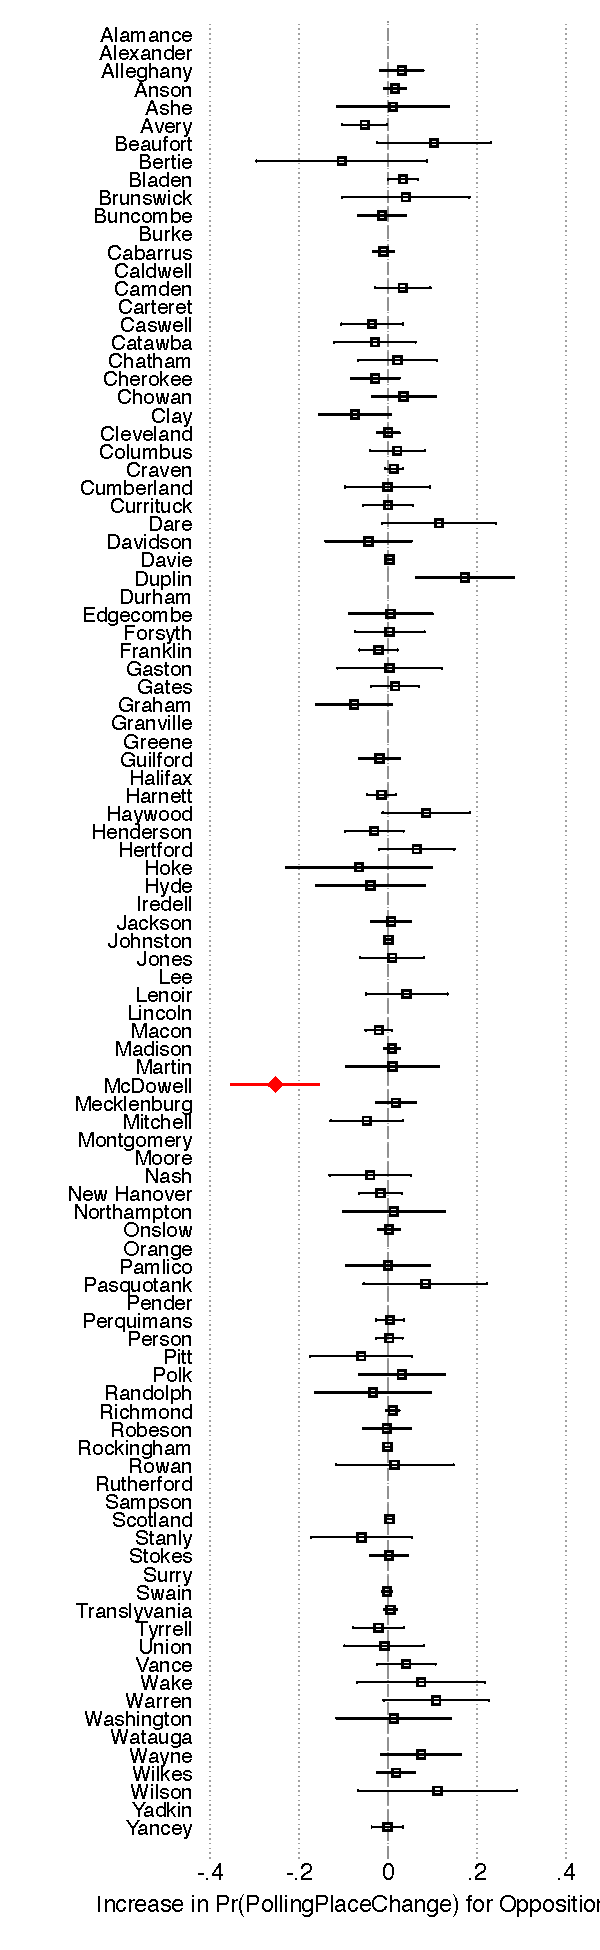
\includegraphics[ width=0.25\textwidth]{../../50_results_full/Plot_County_Coefficients_pp_has_changed_part1_2012.pdf}   \hspace*{1.2in}  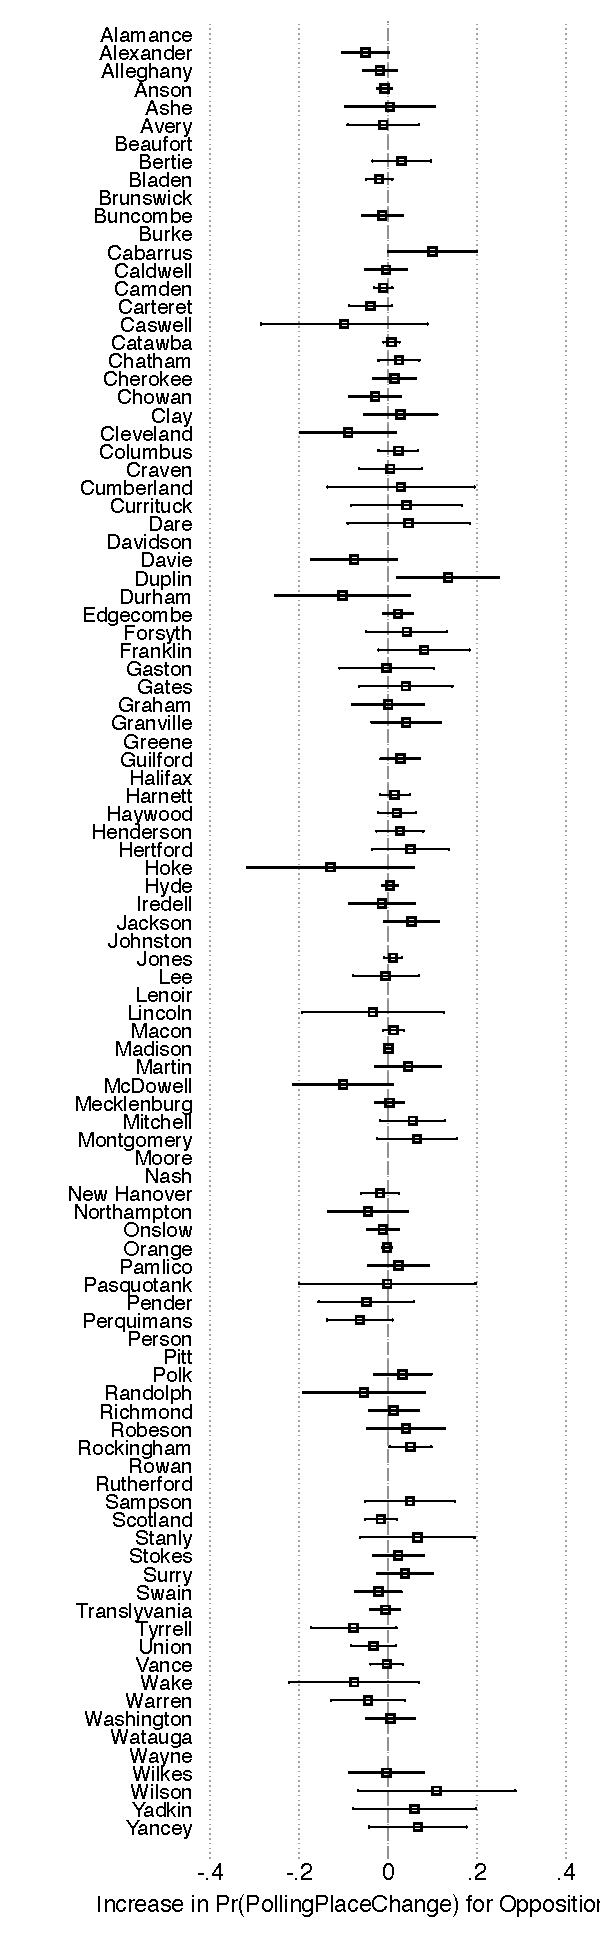
\includegraphics[ width=0.25\textwidth]{../../50_results_full/Plot_County_Coefficients_pp_has_changed_part1_2016.pdf}\\
		\label{county_panel_dem}
		\end{center}
	\scriptsize{\emph{Notes:}   The above plot presents estimates of the increase in the probability of experiencing a polling place change for voters of the opposition party to the Governor (and thus local election officials) ($\hat{\beta_{1}}$) from equation~\ref{equation_panel_party} for each county individually. Standard errors are clustered by precinct-assignment history. Estimates are plotted with naive 95\% confidence intervals. Red estimates (diamond points) are statistically significant after applying the \citet{Benjamini:2006gd} multiple test correction with a False Discovery Rate limit of 0.05; insignificant estimates are black hollow squares.  Coefficients for some counties cannot be estimated because no precincts in those counties experienced a polling place change.} \vspace*{.2in}
\end{figure} \normalsize

Figure~\ref{county_panel_dem} indicates that even though there is no evidence of targeting statewide, the differential incidence of polling place changes varies substantially across counties.  Moreover, the effects we detect in individual counties are often at levels that would appear statistically significant in single-county analysis.  In a single county analysis, for example, we would estimate a statistically significant increase in the probability that Republican voters experienced a polling place change under Democrat-appointed local election administrators in Bladen and Duplin counties in 2012. In 2016, we would similarly conclude that Democratic voters in Cabarrus, Duplin, and Rockingham counties were more likely to be targeted by Republican administrators.  If the researcher chose not to cluster their standard errors, they would find even more statistically distinguishable effects.

Critical for the interpretation of these as evidence of targeting is the fact that for every county in which polling place changes appear to fit a partisan narrative, a counter example can be identified.  There are just as many counties where parties' polling place changes appear to have disproportionately negatively impacted \emph{their own} partisans as opposition-party voters. Moreover, when we apply multiple test corrections to account for the fact that we are analyzing the effects in every county in which a change occurs, only McDowell county shows statistically significant evidence of differential targeting.  In addition, our estimate actually suggests Democrats are targeting their \emph{own} voters with polling place changes.  Appendix~\ref{appendix_countytargetinganddemographics} examines the variation in estimated county-level effects further to show that there is no evidence that these differences are correlated with county demographics nor the ``swing'' status of counties where there might be an additional incentive to target opposition voters to improve outcomes in local races.

Figure~\ref{figure_normalitytests} plots the distribution of the county-specific estimates alongside a standard normal PDF.  Under both partisan regimes, the distribution of estimated effects is centered around a mean of zero (reflecting the estimates from our statewide regression analysis) and the distribution is remarkably symmetric.  The distribution for 2016 under Republican-appointees in particular is remarkably close to normal (formal standardized normal probability plots can be found in Appendix~\ref{appendix_county_point_estimate_distributions}).

%% FIGURE: Distribution of county point estimates against a normal distribution
%%-----------------------------------------------------------------------------
\begin{figure}[t!]
	\begin{center}
	\caption{Distribution of County-Level Estimates of Targeting}\label{figure_normalitytests}
		\small
		\bigskip
    (a) Democrat-Appointed Officials (2012) \hspace*{.5in} (b) Republican-Appointed Officials (2016) \\
		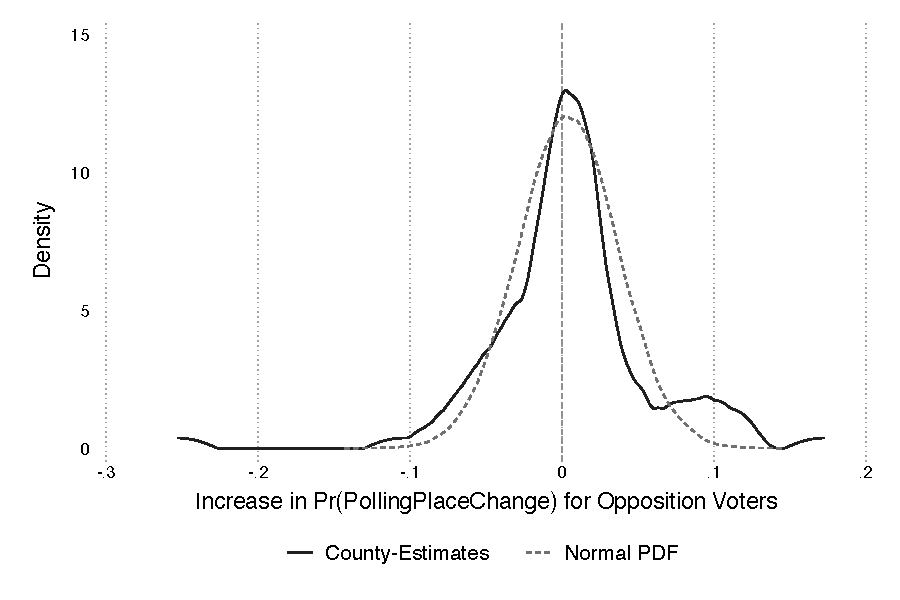
\includegraphics[width=0.45\textwidth]{../../50_results_full/county_point_estimate_density_w_norm_pp_has_changed_2012.pdf}        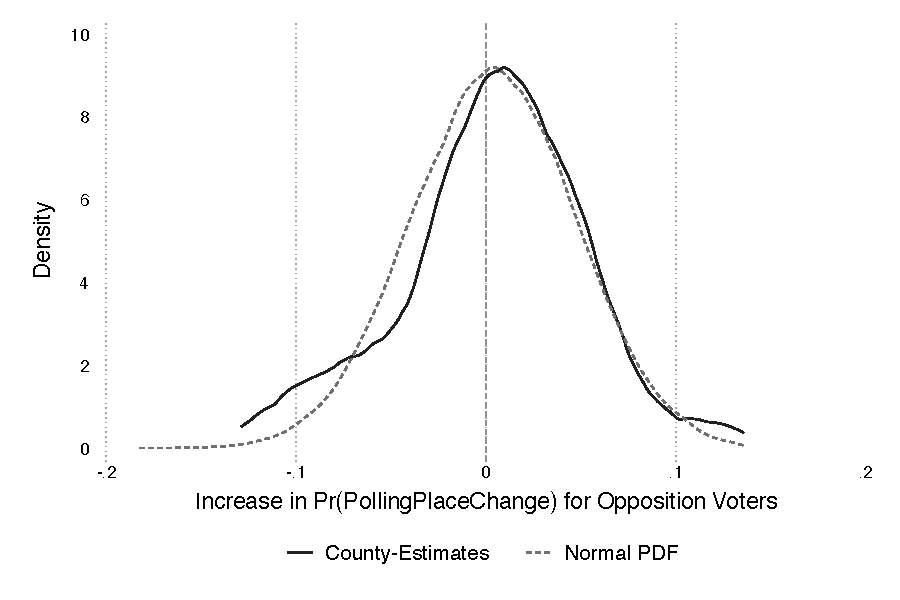
\includegraphics[width=0.45\textwidth]{../../50_results_full/county_point_estimate_density_w_norm_pp_has_changed_2016.pdf}
		\end{center}
    \scriptsize{\emph{Notes:}   The above plot presents the distribution of the estimates of the increase in the probability of experiencing a polling place change for voters of the opposition party to the Governor (and thus local election officials) ($\hat{\beta_{1}}$) from estimating equation~\ref{equation_panel_party} for each county individually. Some county estimates are omitted because they cannot be estimated because no precincts in those counties experienced a polling place change.  Normal distributions are simulated.}
\end{figure} \normalsize

The similarity between the distribution of county-level effects, $\hat{\beta_{1}}$, and the standard normal PDF in Figure \ref{figure_normalitytests} suggests that counties with statistically significant relationships between polling place changes and partisanship are unlikely to be engaged in partisan targeting.  If the variation in these county-level estimates were generated by county-specific, unobserved characteristics---e.g., variation in the willingness of partisan-appointed local officials to manipulate polling places for partisan purposes---the distribution of county-level estimates should reflect the distribution of those characteristics across counties.  It seems extremely unlikely that the resulting distribution of omitted county-level differences like the willingness to use polling place changes to try to influence turnout would be so symmetric and so closely approximate normality.

However, if the cross-county variation in our estimates of $\beta_{1}$ instead results from voter-level (unobserved) characteristics, then the averaging of these voter-level shocks into each of our county-level effects would result in a distribution of county-averages that converges to normality as the number of counties goes to infinity by the Central Limit Theory.  The fact that the distribution of county-level effects we estimate so closely approximates a standard normal distribution---especially in 2016---suggests that the variation in county-level effects plotted in Figure \ref{figure_normalitytests} is more likely the result of aggregating voter-level i.i.d. shocks rather than variation in county-level election administrator characteristics or other county features that make some counties better settings to affect change with precinct and polling places.\footnote{In Appendix~\ref{appendix_politically_responsive_counties} we conduct an analysis in which we effectively select on the dependent variable---that is, we classify counties based on whether journalists and activists made a public claim about a politically motivated change in election administration.  Even still, we cannot find evidence consistent with partisan targeting for electoral gain.   That is, these ``politically responsive counties'' are no more likely, on average, to target opposition voters with precinct and polling place changes than other counties. }

% Finally, as one method of evaluating whether the distribution of county-specific effects is related to an underlying county feature that makes them more able or willing to affect electoral change with precinct and polling place changes, we classify every county based on whether a public claim was made about the occurrence of a politically motivated change in election administration by journalists or activists during the period we study.  We then evaluate whether there is any differential evidence of targeting occurring in these counties previously identified as possibly more willing to engage in such behavior.  In the interest of space,  reports the full set of results.  We fail to find evidence consistent with political targeting even when we focus only on counties where such behavior has been previously alleged.  This evidence again suggests that the changes we observe were not likely used in North Carolina in 2016 to impose costs on Democrats designed to keep them away from the polls.

%% ----------------------------------- SECTION ----------------------------------------- %%

\section{\large Precinct and Polling Place Changes After the Removal of Section 5}\label{sub_shelby}
\vspace*{-0.5cm}

Although the distribution of county-level effects does not suggest a pattern in which some counties are differentially targeting opposition voters with precinct and polling place changes, we probe the possibility that other county-level characteristics might reveal systematic targeting.  Specifically, we evaluate whether the removal of minority voting protections---specifically, Section 5 of the 1965 Voting Rights Act (VRA)---by the 2013 \emph{Shelby County v. Holder} Supreme Court decision allowed Republican local election officials to target Black and Democratic voters in 2016 in a manner that officials could not previously do.  The removal of Section 5 has been popularly cited as unleashing a torrent of voting changes aimed at minority voter suppression, including polling place changes \citep{knafo2013,berman2016,Graham:2016wq,BrennanCenterforJustice:2018ux}.

To investigate the effect of removing the necessity of obtaining federal preclearance before making changes to precinct and polling places, we estimate equation~\ref{equation_panel_partyrace} separately for the 40 counties formerly covered by Section 5 and the 60 counties that were not.\footnote{We do this simply because we consider the split sample analysis easier to interpret than the triple interaction term.}  We restrict our analysis to 2016, the presidential election year post-\emph{Shelby} for which we have data.  This allows us to describe whether, on average, counties that were formerly covered by Section 5 show differential evidence of racial or partisan targeting relative to counties that were never covered.  Using county fixed effects and thus leveraging within-county variation in potential targeting ensures that detected differences are related to former Section 5 coverage rather than fixed county-level characteristics.  Were the \emph{Shelby} decision to have resulted in more opportunities to move the polling places of minority (and likely Democratic) voters, we would expect to find that these groups experience significantly more changes in formerly covered counties as compared to those never covered.

This descriptive investigation cannot tell us the causal effect of Section 5 removal because we lack the appropriate conditions to estimate the counterfactual of how precinct and polling places \emph{would have} been changed absent the \emph{Shelby} decision.  Because we only observe Democratic control of election administration prior to Shelby and Republican control after Shelby, we cannot do a difference-in-difference analysis (as there are effectively two distinct but empirically inseparable post-2013 treatments that we would expect to interact with former Section 5 coverage status).

Polling place changes made by Democrats prior to 2016 are highly unlikely to be affected by Section 5---black voters are likely to be Democrats in North Carolina, and Democrats are unlikely to have wanted to change precincts or polling places of blacks in a way that would have failed pre-clearance by the Department of Justice.  Moreover, if Republicans are as likely to target black voters in any county, regardless of \emph{former} Section 5 coverage status controlling for county fixed effects that account for stable county features like the percentage of the county population that is black, a difference-in-differences design would not provide evidence of a differential pre-post \emph{Shelby} change between covered and uncovered counties.  Trends in changes to precincts and polling places made between pre-\emph{Shelby} Democratic officials (2012) and post-\emph{Shelby} Republicans officials (2016) in uncovered counties do not represent the relevant counterfactual of how covered counties would have behaved had coverage remained, but we present these trends in Appendix~\ref{appendix_shelby}.\footnote{In settings where partisan control of election administration does not change coincident with Section 5 removal, however, such a design could be used.}

We expect our cross-sectional comparison to provide an \emph{over}-estimate of targeting behavior because the cross-sectional estimates will be confounded by both county differences that are a function of why some counties were covered in the first place, as well as differences due to the removal of coverage itself.  This analysis will be therefore biased in favor of finding evidence consistent with partisan-motivated targeting.\footnote{Additionally, former coverage may influence need-based polling place changes.  If the onerous pre-clearance process resulted in counties forgoing genuine need-based changes prior to 2013, then the removal of Section 5 may have resulted in an increase in changes to address disability access, parking and the like.  Again, we note that we have no evidence to suggest that need-based changes would be correlated with the use of a given polling place by voters of particular partisanship or race.}

%However, despite these limitations, this approach nevertheless seems reasonable provided that neither Democrats nor Republicans had \emph{non}-Section 5 reasons for differentially targeting voters in covered versus uncovered counties. That some counties were \emph{formerly} covered should not enter into the decision of officials to \emph{target} in 2016.

Table~\ref{table_shelby} presents the results our descriptive analysis.  Models 1 and 2 being by considering differences in the probability of voters experiencing a polling place change by race in 2016 between covered counties (model 1) and uncovered counties (model 2). We focus on the racial interaction terms since Section 5 was designed to protect minority voters from discriminatory voting changes (see Appendix~\ref{appendix_maintargeting} for full results).

%% TABLE: SHELBY Targeting
%%------------------------
\begin{table}
    \def\sym#1{\ifmmode^{#1}\else\(^{#1}\)\fi}
    \begin{center} \footnotesize
    \caption{Evidence of Targeting in 2016 by Pre-\emph{Shelby v. Holder} Section 5 Coverage }\label{table_shelby}
    \begin{tabular}{@{\extracolsep{5pt}}lcccccc}
        \noalign{\smallskip}\hline\hline\noalign{\smallskip}\noalign{\smallskip}
                &  \multicolumn{2}{c}{$Pr(\Delta PollingPlace)$} & \multicolumn{2}{c}{$Pr(PP Moved Farther)$} & \multicolumn{2}{c}{$\Delta VotersPerPrecinct$}   \\
                \cline{2-3} \cline{4-5} \cline{6-7} \noalign{\smallskip}
                        &\multicolumn{1}{c}{(1)}&\multicolumn{1}{c}{(2)}&\multicolumn{1}{c}{(3)}&\multicolumn{1}{c}{(4)}&\multicolumn{1}{c}{(5)}&\multicolumn{1}{c}{(6)}\\
                &\multicolumn{1}{c}{Section 5}&\multicolumn{1}{c}{Non-Section 5}&\multicolumn{1}{c}{Section 5}&\multicolumn{1}{c}{Non-Section 5}&\multicolumn{1}{c}{Section 5}&\multicolumn{1}{c}{Non-Section 5}\\
\midrule
\emph{WhiteOpposition}&   0.0057         &  -0.0030         &   0.0037         &   0.0053         &    -2.04         &     3.45         \\
                & (0.0053)         & (0.0037)         &  (0.011)         &  (0.010)         &   (3.47)         &   (2.52)         \\
\emph{BlackOpposition}&   0.0082         &   0.0041         &    0.020         &   0.0051         &     1.82         &     0.23         \\
                &  (0.011)         &  (0.016)         &  (0.042)         &  (0.023)         &   (10.4)         &   (5.81)         \\
\midrule
Controls        &\checkmark         &\checkmark         &\checkmark         &\checkmark         &\checkmark         &\checkmark         \\
County FE       &\checkmark         &\checkmark         &\checkmark         &\checkmark         &\checkmark         &\checkmark         \\
Observations    &   772614         &  1565923         &   124691         &   243043         &   772532         &  1565759         \\
Mean of DV      &     0.16         &     0.16         &     0.56         &     0.58         &     40.2         &     28.8         \\
SD of DV        &     0.34         &     0.34         &     0.46         &     0.47         &    220.0         &    194.0         \\
County Clusters &       40         &       60         &       33         &       50         &       40         &       60         \\
\\
        \noalign{\vspace*{-.17in}}\hline\hline\noalign{\smallskip}
    \multicolumn{7}{p{6.3in}}{\scriptsize \emph{Notes:} The table presents coefficients from estimating equation~\ref{equation_panel_partyrace} for 2016 under Republican-appointed local officials.  The unit of analysis is the voter.  Our controls are linear and quadratic $Age$. Full regression results can be found in Appendix~\ref{appendix_shelby}. Estimates of targeting for $Pr(PPMovedFurther)$ are conditional on experiencing a polling place change, accounting for the different sample sizes. Standard errors clustered at the county level. \sym{*} \(p<0.1\), \sym{**} \(p<0.05\), \sym{***} \(p<0.01\)}
    \end{tabular}
    \end{center}
\end{table}

Model 1 shows no evidence that coverage is associated with differential Republican targeting of Black Democrats with polling place changes as compared to white Democrats.  While the estimate on $BlackOpposition$ is larger for covered counties than uncovered counties, when we estimate an interacted model, we cannot reject the null hypothesis that there is no differential impact of polling place changes on Black Democrats in covered as compared to uncovered counties.

Models 3 and 4 provide limited evidence that travel times increased differentially for Black Democrats who had their polling place changed in formerly covered counties, but the estimated effects and substantively and statistically indistinguishable from zero.  While the coefficient in model 3 associated with a polling place being moved further away is larger for $BlackOpposition$ than $WhiteOpposition$, the difference is quite small---being a black Democrat makes you 2 percentage points more likely to have your polling place moved further in a formerly covered county than a Republican of any race.  Models 5 and 6 of Table~\ref{table_shelby} present our results for voters per precinct to reveal that black Democrats in formerly covered counties experienced re-precincting that increased the number of voters per polling place by less than 2 voters on average.   Black Democrats in formerly covered counties did experience a larger increase in voters per precinct relative to uncovered counties, but the difference is essentially just 1 voter.

Given that our empirical design likely over-estimates differences by former coverage status, it is hard to find evidence consistent with the claim that the removal of Section 5 coverage by the \emph{Shelby} decision resulted in Republican-appointed local election administrators increasing polling place changes for Black Democrats or re-precincting black Democrats into larger precincts. Of course, this does not mean that the removal of Section 5 of the VRA did not have an impact on \emph{other} aspects of election administration in North Carolina, or that the removal of Section 5 coverage may not have resulted in targeted changes in polling places in other states. Our results do suggest, however, that popular concerns about an increase in post-\emph{Shelby} voter targeting by Election Day polling place manipulation in North Carolina are not supported by the data. % our investigation fails to uncover the large effects that would be consistent with a story in which administrators were freed to suppress minority turnout by the removal of federal minority voting protections.


%-------------------------------- DISCUSSION ---------------------------------------------%

\section{\large Discussion}\label{section_discussion}
\vspace*{-0.5cm}

In theory, the discretion of partisan local election officials can be used to impose costs on opposition voters in an effort to keep them away from the polls.  Precinct and polling place changes---which can increase wait times at the polls, confusion about where to vote, and travel times to cast a ballot---are a tool local officials could wield against opposition voters.  Despite many claims about the occurrence of such activity, evidence documenting its existence has proven elusive due to the difficulty of inferring partisan-intent and the scope of data required to make such an inference.

Using novel data on voters, polling place locations, and precinct boundaries that we collect across the 2008, 2012, and 2016 presidential elections in North Carolina, we provide the most systematic and extensive examination of the extent to which election officials change Election Day polling places in ways consistent with partisan-motivated targeting. North Carolina is an ideal focus for our investigation not only because of data availability, but also because statewide elections have been decided by razor-thin margins (even small turnout effects could prove pivotal), local election officials have been politicized in making other discretionary decisions, the historical legacy of race-based disenfranchisement is long, lawsuits alleging partisan voter suppression abound, and journalists and activists have continuously raised the alarm about election manipulation for partisan gain \citep{jacobs}. Finally, the unique variation \emph{within} North Carolina over time in the VRA's Section 5 coverage allows us to evaluate the consequences of the \emph{Shelby v. Holder} decision more systematically than the literature has yet been able to do. %If ever we would expect to find evidence that precinct and polling place changes are being used as a tool in contemporary voting wars, we would expect to find it in North Carolina.

Nevertheless, despite our theoretical priors, we do not find evidence consistent with the movement of precincts or polling places for partisan gain. Not only are we unable to reject the null hypothesis of no targeting, but our estimates of the impact by race and partisanship are also exceedingly small in magnitude.  A black Democrat is \emph{less than 1 percentage point} more likely, on average, than a Republican of any race to have experienced a polling place change made by Republican-appointed election administrators. We don't suggest that small effects are normatively acceptable, but the effects are considerably smaller than what might be expected given widespread claims.

We \emph{do} find variation in the racial and partisan impact of precinct and polling place changes when we compare counties to one another. However, the between-county variation that we identify does not relate to the party in control of decision-making as we predicted---as many counties appear to, on average, target same-party voters more with changes, as counties that target opposition party voters.  Moreover, the variation in county effects does not appear to be the result of removing minority voting protections provided by the VRA, despite popular concerns to the contrary.  The distribution of our county-level estimates more likely results from the aggregation of random \emph{voter-level} shocks than the differential willingness or ability of officials to engage in manipulation.

Our results therefore suggest that in North Carolina, in the years we study, it is unlikely that precinct and polling place changes were systematically and widely used as a tool designed to suppress voter turnout amongst voters of particular partisanship or race.  To be clear, this does not mean that this type of manipulation was not attempted, or that it wasn't used in particular instances.  Our study shows that it was not successfully implemented in a systematic fashion.  Nor does this mean that it has not been used as a tool of voter suppression in other jurisdictions or in other years.  Nor is it impossible that the lack of manipulation in the spatial distribution of polling places that we find was not made up for in the strategic selection of polling places with characteristics designed to favor voters of a particular race or partisanship (e.g. black churches or majority-white schools).  Our results do not speak to whether partisan officials in North Carolina or elsewhere might employ these tools in the future in an attempt to maintain their party's political power.  Indeed, reports in which precinct and polling place manipulation seemingly designed to disenfranchise minorities were defeated before being implemented suggest that public vigilance may play an important role in ensuring that our null results remain true in the future \citep{Blackwell:2018uq}.

%Given the extreme challenge of determining the intent of local administrators, our results do not identify \emph{why} we do not observe this type of partisan electoral manipulation despite our predictions to the contrary.  Answering this question remains a fruitful avenue for future research.  Although we lack the research designs to evaluate them, we nevertheless propose a number of possible explanations.  First, the lack of partisan manipulation may be a consequence of officials who are highly motivated or institutionally constrained to fulfill their official duty to administer elections fairly.  Although local officials have the explicit legal authority to make discretionary precinct and polling place changes, the individuals who put themselves forward for these administrative positions may be highly civic-minded.  The institutional structure of North Carolina election administration---in which appointed partisan officials with the legal authority to make precinct and polling place changes work in tandem with longer-serving election directors---may also constrain partisan discretion.\footnote{Anecdotal evidence cuts slightly against this explanation, however.  The use of administrative discretion to manipulate early voting hours and locations has not yet been systematically tested in the literature; however, accounts abound that those decisions---made by the same boards, potentially checked by the same directors---have been politicized \citep{campbell2016,campbell2016c}.}  Election directors may provide a check on overtly partisan changes.


Given the extreme challenge of determining the intent of local administrators, our results do not identify \emph{why} we do not observe this type of partisan electoral manipulation despite our predictions to the contrary. Answering this question remains a fruitful avenue for future research. Although we lack the research designs to evaluate them, we nevertheless propose a number of possible explanations. First, the lack of partisan manipulation may be a consequence of officials who are highly motivated to fulfill their official duty to administer elections fairly (or institutionally constrained from doing otherwise).\footnote{For instance, \cite{kropfPAR} note an increasing professionalization of bureaucrats.  ``Such professionalization,'' they write, ``promotes norms and values, such as efficiency, fairness, and transparency, that could mitigate against the influence of partisanship.''} Even if local officials have the explicit legal authority to make discretionary precinct and polling place changes, the individuals who put themselves forward for these administrative positions may be highly civic-minded. The institutional structure of North Carolina election administration---in which appointed partisan officials with the legal authority to make precinct and polling place changes work in tandem with longer-serving election directors---may also create social pressures that push election officials towards non-partisan choices. That said, anecdotal evidence cuts slightly against this explanation.  Even though the use of administrative discretion to manipulate early voting hours and locations has not yet been systematically tested in the literature accounts abound that those decisions---made by the same boards, potentially checked by the same directors---have indeed been politicized \citep{campbell2016,campbell2016c}.

It is also possible that we do not observe precinct and polling place manipulation because officials did not consider these changes a sufficiently (cost-)effective strategy to affect turnout.  But, while the turnout effects that officials could have expected from polling place changes given the evidence available at the time \citep{brady2011turning} was not enough \emph{on its own} to change any of the statewide election results of which we are aware, it is \emph{also} true that other electoral manipulations were unlikely \emph{on their own} to be decisive.  Given uncertainty in the effectiveness of electoral manipulation strategies, and the small margins in statewide elections, our expectation would be that willing administrators would pursue as many strategies available to them as possible, and thus ``contest-every-vote'' \citep{phillips2016,jacobs}.  Still, the high percentage of early voting in the state may have focused resource-constrained officials' attention on that area (or others) for potential manipulation, leaving Election Day voting decisions to be made for technocratic rationales.  Whether manipulation occurred in other realms of local discretion is an important question for future research.

While there are features of North Carolina that make it both a substantively and analytically ideal case to study, as with any case selection, there are also features unique to North Carolina that condition the scope for generalizability.  In particular, since the majority of North Carolina voters use early voting, which may once again limit the attention and resources officials give to Election Day voting, our results seem most likely to generalize to states with high proportions of early or convenience voters, a large and growing number of states.  Finally, the results are best thought-of as generalizing to states that have somewhat similar institutional structures at the local level.\footnote{Variation in institutional structures across states represent a fruitful avenue for additional research.}

% North Carolina's election administration system is more centralized than in many other states.  This centralization might constrain discretion and moderate the ability to implement a local partisan administrative strategy.  Eight other states have similar administrative structures, however, and we might expect these types of results to generalize to those cases \citep{ncsl2016}.

Our results also highlight an important methodological issue for studies of election forensics broadly.  The fact that we find sizable effects at the county-level that are likely attributable to idiosyncratic voter differences rather than partisan-targeting highlights a real danger for work that attempts to make inferences about \emph{widespread} electoral manipulation from a single locality.  Our results show how the interpretation of a locally-estimated effect depends critically on the larger context of effects.   Although the time and effort required to collect the data on polling places and precincts for further state-level, cross-county investigations are substantial, the value of such investigations to our understanding of whether and how local discretion may influence the most basic practices of U.S. democracy we believe is commensurate with that difficulty.

% While some of the limitations of studying variation within one county apply to studying variation within one state (indeed, one of \emph{anything}, for that matter), states are, on their own, substantively relevant for state and national election outcomes (especially swing states like North Carolina), and also by definition contain a multitude of individual decision-making units (i.e. county boards) across which variation can be assessed.  %There are contexts to which we think our results can reasonably generalize, but we are clear that our conclusion is simply that our results are \emph{internally} valid.

%Finally, although our findings suggest that claims about election administrators undermining democracy in the United States may be overblown, considerable research is still needed in this area. Because the entire state of North Carolina is essentially ``treated'' by regime change at the same time, we lack co-varying geographic and temporal variation in partisan control that could be leveraged in future studies in other contexts. Moreover, much more work is needed to continue to uncover the effects and non-effects of the \textit{Shelby County v. Holder} decision, particularly in other contexts that allow an approximation of the counterfactual of how jurisdictions would have behaved had Section 5 continued in effect.  Although the time and effort required to collect the data required for the investigations we conduct was considerable and expanding the investigation to other states and time periods would impose extreme costs on researchers, the difficulty in doing so is directly related to its importance.












%---------------------------------------------REFERENCES--------------------------------------------------%

% References
%----------------

\bibliographystyle{apsr.bst}
\singlespacing
\bibliography{precinct}


%-------------------------------------------------------------------------------------%
%-------------------------------------APPENDIX----------------------------------------%
%-------------------------------------------------------------------------------------%

\clearpage
\newpage
\normalsize
\onehalfspacing

\appendix

%TC:ignore


\begin{centering}

\section*{\normalfont \LARGE Appendix to \\``The Politics of Locating Polling Places: Race and Partisanship in North Carolina Election Administration, 2008-2016''}
\vspace*{-0.5cm}


	\vspace{.15in} \large
	Michael E. Shepherd \hspace*{.2in} Adriane Fresh  \hspace*{.2in} Nick Eubank \hspace*{.2in} Joshua D. Clinton



\large
\vspace{.2in}
Date: September 15, 2018


\large
\vspace{.2in}

\normalsize
\vspace*{.2in}
Note that this Appendix is to be published online only.

\end{centering}


\setcounter{footnote}{0}
\setcounter{equation}{0}
\setcounter{page}{1}

\renewcommand{\thesubsection}{\Alph{subsection}}




\newpage
\vspace{.2in}
\noindent \textbf{Appendix Contents}

\vspace{.1in}
\noindent \textbf{A} 		\hspace*{.191in} \textbf{Data Sources, Measurement, and Summary Statistics  } \dotfill page~\pageref{appendix_datasources}\\
\textbf{B} 		\hspace*{.2in} \textbf{Details of the Geocoding Procedure  } \dotfill page~\pageref{appendix_geocoding}\\
\textbf{C} 		\hspace*{.205in} \textbf{Full Specifications for Main Analyses} 		\dotfill page~\pageref{appendix_maintargeting} \\
\textbf{D} 		\hspace*{.197in} \textbf{Distribution of Change in Polling Place Registrants} 			\dotfill page~\pageref{appendix_change_voters_per_pp} \\
\textbf{E} 		\hspace*{.214in} \textbf{Normality of County-Level Point Estimates } 	\dotfill page~\pageref{appendix_county_point_estimate_distributions} \\
\textbf{F} 		\hspace*{.21in} \textbf{County Targeting Estimates and County Demographics } 	\dotfill page~\pageref{appendix_countytargetinganddemographics} \\
\textbf{G} 		\hspace*{.18in} \textbf{Subsetting on Political Responsive Counties} 	\dotfill page~\pageref{appendix_politically_responsive_counties} \\
\textbf{H} \hspace*{.18in} \textbf{Additional \emph{Shelby v. Holder} Graphical Evidence } 	\dotfill page~\pageref{appendix_shelby} \\




%% --------------------------------------- APPENDIX: Shelby v. Holder --------------------------------------- %%
\clearpage \newpage
\subsection{Data Sources, Measurement, and Summary Statistics}\label{appendix_datasources}
\setcounter{table}{0}
\setcounter{figure}{0}
\renewcommand{\thetable}{A\arabic{table}}
\renewcommand{\thefigure}{A\arabic{figure}}


This appendix presents information on the measurement and data sources of our non-precinct and polling place variables.  (Information on precinct and polling place can be found in the main text of the paper.)  We also present basic summary statistics for all of our variables.


%% TABLE: Control Variables, Data Sources and Measurement
%%--------------------------------------------------------

\begin{table}[h!]\centering \footnotesize
\def\sym#1{\ifmmode^{#1}\else\(^{#1}\)\fi}
	\caption{\small Measurement and Data Sources for Variables}\label{table_covariates}
	\smallskip
	\begin{tabular}{@{\extracolsep{5pt}}l*{3}{l}}
	\noalign{\smallskip}\hline\hline\noalign{\smallskip}\noalign{\smallskip}
	Variable & Measurement & Source   \\
	\midrule
	Race & \multicolumn{1}{p{2.9in}}{Individual self-identification of race or ethnicity.  The categories of race are: $white$, $black$, $hispanic$, $unknown$, $other$, $Native American$, $asian$ and $multi-race$.  We use the categories as separate indicator variables in our analyses. Individuals who self-identify with different racial categories in different years are assigned their modal selected category.  As is typical in government self-identification, voters in North Carolina select first a race and then,  they may separately choose whether they identify as Hispanic (as an ethnicity).  We first code people by their race, then anyone white who identifies as Hispanic we code as Hispanic.  This coding is slightly biased towards finding targeting, since we increase those coded as minority in our sample.  Though we don't find evidence of targeting.  The number of people identifying as any non-white race and Hispanic is small enough that our results are not sensitive to different coding. We include $hispanic$ in what we call our \emph{race} category for ease of exposition, and also because we don't think that the difference between race and ethnicity is a meaningful one in how election officials would make potential targeting decisions.  } & \multicolumn{1}{p{2.0in}}{Self-identification, North Carolina State Board of Elections voter rolls.} \\
	\noalign{\smallskip}\noalign{\smallskip}
	Partisanship & \multicolumn{1}{p{2.9in}}{Individual party registration at the time of voter registration.  The partisan categories are: $Republican$, $Democrat$, $Unaffiliated$ and $Libertarian$.  Each are measured as indicators.} & \multicolumn{1}{p{2.0in}}{North Carolina State Board of Elections voter rolls.} \\
	\noalign{\smallskip}\noalign{\smallskip}
	$Age$ and $Age^{2}$ & \multicolumn{1}{p{2.9in}}{Individual age reported at the time of voter registration.} & \multicolumn{1}{p{2.0in}}{North Carolina State Board of Elections voter rolls.} \\
	\noalign{\smallskip}
	\hline\hline\noalign{\smallskip}
\end{tabular}
\end{table}



 TABLE: Summary Statistics
--------------------------------------
\begin{table}[h!]\centering \footnotesize
\caption{Summary Statistics}\label{table_summary}
\vspace*{.055in}
\begin{tabular}{l c c c c c }
\hline\hline\noalign{\smallskip}
	\multicolumn{1}{c}{Variable} & Mean & Std. Dev. & Min &  Max & N \\
	\hline \noalign{\smallskip}
		$Voted$  &    0.80 &   0.403 &   0.000 &   1.000 &      4,681,792  \\
		$VotedEarly$ &    0.46 &   0.498 &   0.000 &   1.000 &      4,681,792  \\
		$VotedElecDay$&    0.30 &   0.457 &   0.000 &   1.000 &      4,681,792  \\
		$VotedMailIn$ &    0.04 &   0.185 &   0.000 &   1.000 &      4,681,792  \\
		$VotedLastElec$&    0.89 &   0.313 &   0.000 &   1.000 &      4,681,792  \\
		$\Delta PollingPlace$&    0.16 &   0.368 &   0.000 &   1.000 &      4,681,792  \\
		$\Delta DriveTime$&    0.02 &   1.135 & -23.217 &  22.717 &      4,681,792  \\
		$Age$&   57.02 &  16.221 &  20.000 & 116.000 &      4,681,792  \\
		$Age^{2}$& 3514.55 & 1895.658 & 400.000 &  1.3e+04 &      4,681,792  \\
		$White$&    0.76 &   0.426 &   0.000 &   1.000 &      4,681,792  \\
		$NonWhite$&    0.24 &   0.426 &   0.000 &   1.000 &      4,681,792  \\
		$Black$&    0.24 &   0.426 &   0.000 &   1.000 &      4,681,792  \\
		$Hispanic$&    0.00 &   0.047 &   0.000 &   1.000 &      4,681,792  \\
		$Unknown$&    0.01 &   0.115 &   0.000 &   1.000 &      4,681,792  \\
		$Other$&    0.01 &   0.111 &   0.000 &   1.000 &      4,681,792  \\
		$Asian$&    0.01 &   0.080 &   0.000 &   1.000 &      4,681,792  \\
		$NativeAm$&    0.01 &   0.074 &   0.000 &   1.000 &      4,681,792  \\
		$MultiRace$&    0.00 &   0.053 &   0.000 &   1.000 &      4,681,792  \\
		$Republican$&    0.35 &   0.476 &   0.000 &   1.000 &      4,681,792  \\
		$Democrat$&    0.44 &   0.497 &   0.000 &   1.000 &      4,681,792  \\
		$Unaffiliated$&    0.21 &   0.406 &   0.000 &   1.000 &      4,681,792  \\
		$Libertarian$&    0.00 &   0.030 &   0.000 &   1.000 &      4,681,792  \\
	\noalign{\smallskip}\hline\hline\noalign{\smallskip}
	\multicolumn{6}{p{4.6in}}{\scriptsize{\emph{Notes:} The unit of analysis for all variables is the voter-election, except for $income$ which is measured at the census block group.  Summary statistics are calculated for 2012 and 2016, pooled.}}
\end{tabular}
\end{table}




%% TABLE: Our sample compared to voter roll-eligible voters
%%-----------------------------------------------------------------------------
\begin{table}[t!]\centering \small
\caption{Our Sample Compared to Voter Roll-Eligible Voters}\label{table_sample_comparison}
\vspace*{.055in}
\begin{tabular}{l c c }
\hline\hline\noalign{\smallskip}
	\multicolumn{1}{c}{Variable} & Our Panel & Voter Rolls \\
	\hline \noalign{\smallskip}
	$VotedAny$  &    0.80 &    0.72  \\
	$Movers$  & 0.00 &    0.31 \\
	$Age$&   57.02 &   50.49  \\
	$Female$&    0.55 &    0.57  \\
	$White$&    0.76 &    0.66  \\
	$NonWhite$&    0.24 &    0.35 \\
	$Republican$&    0.35 &     0.29  \\
	$Democrat$&    0.44 &     0.39  \\
	$\mathit{Unaffiliated}$&     0.21 &     0.23  \\
	\hline \noalign{\smallskip}
	Sample &      4,681,792 &     12,860,588 \\
		\noalign{\smallskip}\hline\hline\noalign{\smallskip}
	\multicolumn{3}{p{2.7in}}{\scriptsize{\emph{Notes:} The unit of analysis for all variables is the voter-election. Summary statistics are pooled means calculated for 2012 and 2016---i.e. an individual voter enters once for 2012 and once for 2016. The Voter Rolls column includes voters who were eligible to vote in at least one of the three presidential elections in our sample. Note that a traditional balance analyses (e.g. share of each demographic group experiencing a polling place change in the restricted sample and in the full sample) is not possible as polling place change is not defined for many individuals in the full voter role, motivating their exclusion.}}
\end{tabular}
\end{table}





%------------------------------------ APPENDIX B: Geocoding ------------------------------------------%
\clearpage \newpage
\subsection{Details of the Geocoding Procedure}\label{appendix_geocoding}
\setcounter{table}{0}
\setcounter{figure}{0}
\renewcommand{\thetable}{B\arabic{table}}
\renewcommand{\thefigure}{B\arabic{figure}}

Data on 2008 polling places come from the NCSBE data archives -- snapshot date: April 3rd, 2008 --  data on 2012 polling places come from the Data Director of the North Carolina Democratic Party, and data on 2016 polling places were collected from the mid-2017 Internet Archives image of the NCSBE Polling Place Search website.

Shapefiles of precinct boundaries were collected from the NCSBE website for 2012 and 2016 -- snapshot dates: October 4th, 2016 for 2016 election; September 1st, 2012 for 2012 -- and from the NCSBE 2008 precinct boundary shapefile submitted to the 2011 redistricting database to associate polling places and precincts. In some cases, poor record keeping combined with the fact that not all polling places are located with the borders of the precinct they serve makes it impossible to ascertain the precinct served by a given polling places. When a precinct's polling place cannot be ascertained with certainty, we drop that precinct from the analysis. This generates a sample of    3,362,808\unskip~voters with a geolocated polling place, or      79.1\unskip\%~of voters with accurate residence geocodes.




%------------------------------------ APPENDIX C: Full Specifications ------------------------------------------%
\clearpage \newpage
\subsection{Full Specifications}\label{appendix_maintargeting}
\setcounter{table}{0}
\setcounter{figure}{0}
\renewcommand{\thetable}{C\arabic{table}}
\renewcommand{\thefigure}{C\arabic{figure}}


In this appendix we present the coefficient estimates on the control variables for the models presented in the main paper.

%% TABLE
%%------
\begin{table}[h!]\centering \scriptsize
\def\sym#1{\ifmmode^{#1}\else\(^{#1}\)\fi}
	\caption{The Average Probability of Experiencing a Polling Place Change}\label{MainTargetControl}
	\smallskip
	\begin{tabular}{@{\extracolsep{5pt}}l*{8}{c}}
	\noalign{\smallskip}\hline\hline\noalign{\smallskip}\noalign{\smallskip}
			&  \multicolumn{7}{c}{$Pr(\Delta Polling Place)$}   \\
			\cline{2-9}  \noalign{\smallskip}
                &\multicolumn{1}{c}{(1)}         &\multicolumn{1}{c}{(2)}         &\multicolumn{1}{c}{(3)}         &\multicolumn{1}{c}{(4)}         &\multicolumn{1}{c}{(5)}         &\multicolumn{1}{c}{(6)}         &\multicolumn{1}{c}{(7)}         &\multicolumn{1}{c}{(8)}         \\
\midrule
\emph{Opposition}&  -0.0083         &   0.0030         &   0.0028         &   0.0031         &   0.0020         &                  &                  &                  \\
                & (0.0055)         & (0.0021)         & (0.0025)         & (0.0047)         & (0.0046)         &                  &                  &                  \\
\emph{Age}      &                  &                  &  0.00016         &  0.00061         & -0.00020         &  0.00018         &  0.00060         & -0.00017         \\
                &                  &                  &(0.00020)         &(0.00037)         &(0.00027)         &(0.00020)         &(0.00038)         &(0.00027)         \\
\emph{Age}$^{2}$&                  &                  &-0.00000089         &-0.0000054         &0.0000027         &-0.00000092         &-0.0000053         &0.0000025         \\
                &                  &                  &(0.0000017)         &(0.0000036)         &(0.0000024)         &(0.0000017)         &(0.0000036)         &(0.0000024)         \\
\emph{Unaffiliated}&                  &                  & -0.00040         & -0.00063         & -0.00046         &                  &                  &                  \\
                &                  &                  & (0.0020)         & (0.0033)         & (0.0020)         &                  &                  &                  \\
\emph{WhiteOpposition}&                  &                  &                  &                  &                  &   0.0016         &   0.0033         & -0.00035         \\
                &                  &                  &                  &                  &                  & (0.0023)         & (0.0050)         & (0.0030)         \\
\emph{BlackOpposition}&                  &                  &                  &                  &                  &   0.0061         &   0.0012         &   0.0054         \\
                &                  &                  &                  &                  &                  & (0.0092)         & (0.0063)         &  (0.010)         \\
\emph{OtherOpposition}&                  &                  &                  &                  &                  &   0.0076         &-0.000078         &   0.0046         \\
                &                  &                  &                  &                  &                  &  (0.012)         & (0.0089)         &  (0.016)         \\
\emph{WhiteUnaffiliated}&                  &                  &                  &                  &                  &  -0.0018         & -0.00021         &  -0.0016         \\
                &                  &                  &                  &                  &                  & (0.0017)         & (0.0045)         & (0.0025)         \\
\emph{BlackUnaffiliated}&                  &                  &                  &                  &                  &  0.00045         &  0.00085         &  0.00060         \\
                &                  &                  &                  &                  &                  & (0.0045)         & (0.0062)         & (0.0037)         \\
\emph{OtherUnaffiliated}&                  &                  &                  &                  &                  &   0.0023         &  -0.0053         &    0.013         \\
                &                  &                  &                  &                  &                  & (0.0051)         &  (0.011)         &  (0.013)         \\
\midrule
County FE       &                  &\checkmark         &\checkmark         &\checkmark         &\checkmark         &\checkmark         &\checkmark         &\checkmark         \\
Year FE         &                  &\checkmark         &\checkmark         &                  &                  &\checkmark         &                  &                  \\
Ct. x Yr. FE    &                  &\checkmark         &\checkmark         &                  &                  &\checkmark         &                  &                  \\
Controls        &                  &                  &\checkmark         &\checkmark         &\checkmark         &\checkmark         &\checkmark         &\checkmark         \\
Year Sample     &    Panel         &    Panel         &    Panel         &     2012         &     2016         &    Panel         &     2012         &     2016         \\
Observations    &  4677529         &  4677529         &  4677529         &  2338992         &  2338537         &  4677529         &  2338992         &  2338537         \\
Mean of DV      &     0.16         &     0.16         &     0.16         &     0.17         &     0.16         &     0.16         &     0.17         &     0.16         \\
SD of DV        &     0.37         &     0.36         &     0.36         &     0.35         &     0.34         &     0.36         &     0.35         &     0.34         \\
 \\
	\noalign{\vspace*{-.1in}}\hline\hline\noalign{\smallskip}
\multicolumn{9}{p{4.0in}}{\scriptsize Standard errors clustered at the individual level. } \\
\multicolumn{9}{l}{\scriptsize \sym{*} \(p<0.1\), \sym{**} \(p<0.05\), \sym{***} \(p<0.01\)}\\
\multicolumn{9}{p{6.1in}}{\scriptsize  \emph{Notes}:  The table presents coefficients from estimating Equation~\ref{equation_panel_party} (columns 1-3) and Equation~\ref{equation_panel_partyrace} (columns 4-6) using OLS.  The unit of analysis is the voter-election in the panel models, and the voter in the cross-sectional models.   The SD of the DV is the average of the within-$i$ standard deviations of the outcome variable for the full panel models. }
\end{tabular}
\end{table}




%% TABLE
%%------
\begin{table}[h!]\centering \scriptsize
\def\sym#1{\ifmmode^{#1}\else\(^{#1}\)\fi}
	\caption{The Probability of Experiencing a Polling Place Change Moved Farther}
	\smallskip
	\begin{tabular}{@{\extracolsep{5pt}}l*{8}{c}}
	\noalign{\smallskip}\hline\hline\noalign{\smallskip}\noalign{\smallskip}
			&  \multicolumn{7}{c}{$Pr(PPMoved Farther)$}   \\
			\cline{2-9}  \noalign{\smallskip}
				                &\multicolumn{1}{c}{(1)}         &\multicolumn{1}{c}{(2)}         &\multicolumn{1}{c}{(3)}         &\multicolumn{1}{c}{(4)}         &\multicolumn{1}{c}{(5)}         &\multicolumn{1}{c}{(6)}         &\multicolumn{1}{c}{(7)}         &\multicolumn{1}{c}{(8)}         \\
\midrule
\emph{Opposition}&   0.0036         &   0.0071         &   0.0067         &   0.0066         &   0.0066         &                  &                  &                  \\
                & (0.0094)         & (0.0075)         & (0.0088)         &  (0.011)         &  (0.011)         &                  &                  &                  \\
\emph{Age}      &                  &                  &-0.000085         &  0.00034         & -0.00071         &-0.000098         &  0.00035         & -0.00074         \\
                &                  &                  & (0.0010)         & (0.0013)         & (0.0012)         & (0.0010)         & (0.0013)         & (0.0012)         \\
\emph{Age}$^{2}$&                  &                  &0.00000023         &-0.0000031         &0.0000049         &0.00000034         &-0.0000031         &0.0000052         \\
                &                  &                  &(0.0000084)         &(0.000011)         &(0.000011)         &(0.0000083)         &(0.000011)         &(0.000011)         \\
\emph{Unaffiliated}&                  &                  &  -0.0013         &  0.00041         &  -0.0032         &                  &                  &                  \\
                &                  &                  & (0.0051)         & (0.0087)         & (0.0033)         &                  &                  &                  \\
\emph{WhiteOpposition}&                  &                  &                  &                  &                  &   0.0043         &   0.0062         &   0.0047         \\
                &                  &                  &                  &                  &                  & (0.0052)         &  (0.011)         & (0.0077)         \\
\emph{BlackOpposition}&                  &                  &                  &                  &                  &    0.014         &    0.015         &    0.012         \\
                &                  &                  &                  &                  &                  &  (0.022)         &  (0.014)         &  (0.023)         \\
\emph{OtherOpposition}&                  &                  &                  &                  &                  &   -0.026         &   0.0016         &   -0.031         \\
                &                  &                  &                  &                  &                  &  (0.018)         &  (0.017)         &  (0.025)         \\
\emph{WhiteUnaffiliated}&                  &                  &                  &                  &                  &  -0.0045         & -0.00068         &  -0.0079         \\
                &                  &                  &                  &                  &                  & (0.0043)         &  (0.011)         & (0.0081)         \\
\emph{BlackUnaffiliated}&                  &                  &                  &                  &                  &  -0.0021         &  -0.0045         &   0.0030         \\
                &                  &                  &                  &                  &                  & (0.0093)         &  (0.016)         & (0.0077)         \\
\emph{OtherUnaffiliated}&                  &                  &                  &                  &                  & -0.00090         &    0.014         &   -0.011         \\
                &                  &                  &                  &                  &                  &  (0.015)         &  (0.019)         &  (0.021)         \\
\midrule
County FE       &                  &\checkmark         &\checkmark         &\checkmark         &\checkmark         &\checkmark         &\checkmark         &\checkmark         \\
Year FE         &                  &\checkmark         &\checkmark         &                  &                  &\checkmark         &                  &                  \\
Ct. x Yr. FE    &                  &\checkmark         &\checkmark         &                  &                  &\checkmark         &                  &                  \\
Controls        &                  &                  &\checkmark         &\checkmark         &\checkmark         &\checkmark         &\checkmark         &\checkmark         \\
Year Sample     &    Panel         &    Panel         &    Panel         &     2012         &     2016         &    Panel         &     2012         &     2016         \\
Observations    &   754298         &   754298         &   754298         &   386564         &   367734         &   754298         &   386564         &   367734         \\
Mean of DV      &     0.55         &     0.55         &     0.55         &     0.53         &     0.57         &     0.55         &     0.53         &     0.57         \\
SD of DV        &     0.50         &     0.48         &     0.48         &     0.47         &     0.47         &     0.48         &     0.47         &     0.47         \\
 \\
	\noalign{\vspace*{-.1in}}\hline\hline\noalign{\smallskip}
\multicolumn{9}{p{4.0in}}{\scriptsize Standard errors clustered at the individual level. } \\
\multicolumn{9}{l}{\scriptsize \sym{*} \(p<0.1\), \sym{**} \(p<0.05\), \sym{***} \(p<0.01\)}\\
\multicolumn{9}{p{6.3in}}{\scriptsize  \emph{Notes}: The table presents coefficients from estimating Equation~\ref{equation_panel_party} (columns 1-3) and Equation~\ref{equation_panel_partyrace} (columns 4-6) using OLS.  The unit of analysis is the voter-election in the panel models, and the voter in the cross-sectional models.   The SD of the DV is the average of the within-$i$ standard deviations of the outcome variable for the full panel models. }
\end{tabular} \label{MainFurtherControl}
\end{table}



%% TABLE
%%------
\begin{table}[h!]\centering \scriptsize
\def\sym#1{\ifmmode^{#1}\else\(^{#1}\)\fi}
	\caption{Change in People Per Precinct}\label{table_pplprecinct_full}
	\smallskip
	\begin{tabular}{@{\extracolsep{5pt}}l*{8}{c}}
	\noalign{\smallskip}\hline\hline\noalign{\smallskip}\noalign{\smallskip}
			&  \multicolumn{7}{c}{$\Delta People Per Precinct$}   \\
			\cline{2-9}  \noalign{\smallskip}
				                &\multicolumn{1}{c}{(1)}         &\multicolumn{1}{c}{(2)}         &\multicolumn{1}{c}{(3)}         &\multicolumn{1}{c}{(4)}         &\multicolumn{1}{c}{(5)}         &\multicolumn{1}{c}{(6)}         &\multicolumn{1}{c}{(7)}         &\multicolumn{1}{c}{(8)}         \\
\midrule
\emph{Opposition}&     0.76         &     0.39         &    -0.26         &    -1.28         &     1.37         &                  &                  &                  \\
                &   (8.14)         &   (1.75)         &   (2.21)         &   (2.97)         &   (3.13)         &                  &                  &                  \\
\emph{Age}      &                  &                  &    0.053         &    -0.14         &     0.10         &    0.052         &    -0.15         &    0.097         \\
                &                  &                  &   (0.18)         &   (0.14)         &   (0.27)         &   (0.17)         &   (0.14)         &   (0.26)         \\
\emph{Age}$^{2}$&                  &                  & -0.00013         &   0.0022\sym{*}  &  -0.0012         & -0.00012         &   0.0023\sym{*}  &  -0.0012         \\
                &                  &                  & (0.0016)         & (0.0012)         & (0.0024)         & (0.0016)         & (0.0012)         & (0.0024)         \\
\emph{Unaffiliated}&                  &                  &    -1.61         &    -4.12         &     1.22         &                  &                  &                  \\
                &                  &                  &   (1.93)         &   (3.42)         &   (1.09)         &                  &                  &                  \\
\emph{WhiteOpposition}&                  &                  &                  &                  &                  &     0.60         &    -1.03         &     1.76         \\
                &                  &                  &                  &                  &                  &   (1.25)         &   (2.99)         &   (2.11)         \\
\emph{BlackOpposition}&                  &                  &                  &                  &                  &     1.26         &     0.99         &     1.30         \\
                &                  &                  &                  &                  &                  &   (4.93)         &   (3.57)         &   (5.44)         \\
\emph{OtherOpposition}&                  &                  &                  &                  &                  &    -3.48         &    -9.05         &    -10.9         \\
                &                  &                  &                  &                  &                  &   (9.49)         &   (5.46)         &   (15.0)         \\
\emph{WhiteUnaffiliated}&                  &                  &                  &                  &                  &    -1.34         &    -3.06         &    -1.33         \\
                &                  &                  &                  &                  &                  &   (1.09)         &   (3.49)         &   (1.39)         \\
\emph{BlackUnaffiliated}&                  &                  &                  &                  &                  &     0.36         &    -4.41         &     4.31         \\
                &                  &                  &                  &                  &                  &   (2.39)         &   (2.78)         &   (3.89)         \\
\emph{OtherUnaffiliated}&                  &                  &                  &                  &                  &    -6.53         &    -20.0         &     13.4         \\
                &                  &                  &                  &                  &                  &   (10.6)         &   (15.7)         &   (13.2)         \\
\midrule
County FE       &                  &\checkmark         &\checkmark         &\checkmark         &\checkmark         &\checkmark         &\checkmark         &\checkmark         \\
Year FE         &                  &\checkmark         &\checkmark         &                  &                  &\checkmark         &                  &                  \\
Ct. x Yr. FE    &                  &\checkmark         &\checkmark         &                  &                  &\checkmark         &                  &                  \\
Controls        &                  &                  &\checkmark         &\checkmark         &\checkmark         &\checkmark         &\checkmark         &\checkmark         \\
Year Sample     &    Panel         &    Panel         &    Panel         &     2012         &     2016         &    Panel         &     2012         &     2016         \\
Observations    &  4677166         &  4677166         &  4677166         &  2338875         &  2338291         &  4677166         &  2338875         &  2338291         \\
Mean of DV      &     7.58         &     7.58         &     7.58         &    -17.4         &     32.6         &     7.58         &    -17.4         &     32.6         \\
SD of DV        &    256.2         &    226.9         &    226.9         &    182.0         &    203.0         &    226.9         &    182.0         &    203.0         \\
 \\
	\noalign{\vspace*{-.1in}}\hline\hline\noalign{\smallskip}
\multicolumn{9}{p{4.0in}}{\scriptsize Standard errors clustered at the county level. } \\
\multicolumn{9}{l}{\scriptsize \sym{*} \(p<0.1\), \sym{**} \(p<0.05\), \sym{***} \(p<0.01\)}\\
\multicolumn{9}{p{6.0in}}{\scriptsize \emph{Notes}: The table presents coefficients from estimating Equation~\ref{equation_panel_party} (columns 1-3) and Equation~\ref{equation_panel_partyrace} (columns 4-6) using OLS.  The unit of analysis is the voter-election in the panel models, and the voter in the cross-sectional models.   The SD of the DV is the average of the within-$i$ standard deviations of the outcome variable for the full panel models. }
\end{tabular}
\end{table}




%% TABLE
\begin{table}[h!]\centering \scriptsize
\def\sym#1{\ifmmode^{#1}\else\(^{#1}\)\fi}
   \caption{Evidence of Republican Targeting Among ``Responsive'' Counties from 2012-2016}\label{table_responsive_wcontrols}
   \smallskip
   \begin{tabular}{@{\extracolsep{5pt}}l*{6}{c}}
   \noalign{\smallskip}\hline\hline\noalign{\smallskip}\noalign{\smallskip}
   &  \multicolumn{2}{c}{$Pr(\Delta PollingPlace)$} & \multicolumn{2}{c}{$Pr(PP Moved Farther)$} & \multicolumn{2}{c}{$\Delta VotersPerPrecinct$}   \\
   \cline{2-3} \cline{4-5} \cline{6-7} \noalign{\smallskip}
                               &\multicolumn{1}{c}{(1)}         &\multicolumn{1}{c}{(2)}         &\multicolumn{1}{c}{(3)}         &\multicolumn{1}{c}{(4)}         &\multicolumn{1}{c}{(5)}         &\multicolumn{1}{c}{(6)}         \\
\midrule
\emph{Opposition}& -0.00087         &                  &   0.0020         &                  &    -1.62         &                  \\
                & (0.0099)         &                  &  (0.028)         &                  &   (11.7)         &                  \\
\emph{Age}      & -0.00040         & -0.00039         & -0.00016         & -0.00014         &    -0.98         &    -0.94         \\
                &(0.00070)         &(0.00067)         & (0.0021)         & (0.0020)         &   (0.77)         &   (0.71)         \\
\emph{Age}$^{2}$&0.0000029         &0.0000027         &-0.0000031         &-0.0000039         &   0.0083         &   0.0081         \\
                &(0.0000052)         &(0.0000053)         &(0.000018)         &(0.000018)         & (0.0069)         & (0.0069)         \\
\emph{Unaffiliated}&   0.0025         &                  &   -0.011         &                  &     2.94         &                  \\
                & (0.0055)         &                  & (0.0068)         &                  &   (4.09)         &                  \\
\emph{WhiteOpposition}&                  &  -0.0011         &                  &    0.012         &                  &    -2.91         \\
                &                  & (0.0046)         &                  &  (0.012)         &                  &   (6.04)         \\
\emph{BlackOpposition}&                  &   0.0017         &                  &  -0.0075         &                  &     1.42         \\
                &                  &  (0.018)         &                  &  (0.048)         &                  &   (18.0)         \\
\emph{OtherOpposition}&                  &   -0.043         &                  &   -0.037         &                  &    -42.7         \\
                &                  &  (0.029)         &                  &  (0.067)         &                  &   (42.8)         \\
\emph{WhiteUnaffiliated}&                  &  0.00095         &                  &   -0.029\sym{*}  &                  &     1.30         \\
                &                  & (0.0043)         &                  &  (0.014)         &                  &   (2.45)         \\
\emph{BlackUnaffiliated}&                  &    0.012         &                  &    0.015         &                  &     18.1         \\
                &                  & (0.0091)         &                  &  (0.010)         &                  &   (14.4)         \\
\emph{OtherUnaffiliated}&                  &    0.052\sym{**} &                  &    0.052         &                  &     65.2\sym{**} \\
                &                  &  (0.021)         &                  &  (0.042)         &                  &   (30.9)         \\
\midrule
Controls        &\checkmark         &\checkmark         &\checkmark         &\checkmark         &\checkmark         &\checkmark         \\
County FE       &\checkmark         &\checkmark         &\checkmark         &\checkmark         &\checkmark         &\checkmark         \\
Observations    &   447793         &   447793         &    78801         &    78801         &   447749         &   447749         \\
Mean of DV      &     0.18         &     0.18         &     0.59         &     0.59         &     71.3         &     71.3         \\
SD of DV        &     0.35         &     0.35         &     0.45         &     0.45         &    286.8         &    286.8         \\
County Clusters &       20         &       20         &       19         &       19         &       20         &       20         \\
 \\
   \noalign{\vspace*{-.1in}}\hline\hline\noalign{\smallskip}
\multicolumn{7}{p{4.0in}}{\scriptsize Standard errors clustered at the individual level. } \\
\multicolumn{7}{l}{\scriptsize \sym{*} \(p<0.1\), \sym{**} \(p<0.05\), \sym{***} \(p<0.01\)}\\
\multicolumn{7}{p{5.6in}}{\scriptsize  \emph{Notes:} The table presents coefficients from estimating Equation~\ref{equation_panel_party} (columns 1, 3 and 5) and Equation~\ref{equation_panel_partyrace} (columns 2, 4 and 6) using OLS.  The unit of analysis is the voter. Our controls are linear and quadratic $Age$. Estimates of targeting for $Pr(PPMovedFurther)$ are conditional on experiencing a polling place change, accounting for the different sample sizes. Standard errors are clustered at the county.}
\end{tabular}
\end{table}



%% TABLE
%%------
\begin{table}[h!]
    \def\sym#1{\ifmmode^{#1}\else\(^{#1}\)\fi}
    \begin{center} \scriptsize
    \caption{Evidence of Targeting in 2016 by Pre-\emph{Shelby v. Holder} Section 5 Coverage }
    \begin{tabular}{@{\extracolsep{5pt}}lcccccc}
        \noalign{\smallskip}\hline\hline\noalign{\smallskip}\noalign{\smallskip}
                &  \multicolumn{2}{c}{$Pr(\Delta PollingPlace)$} & \multicolumn{2}{c}{$Pr(PP Moved Farther)$} & \multicolumn{2}{c}{$\Delta VotersPerPrecinct$}   \\
                \cline{2-3} \cline{4-5} \cline{6-7} \noalign{\smallskip}
                        &\multicolumn{1}{c}{(1)}&\multicolumn{1}{c}{(2)}&\multicolumn{1}{c}{(3)}&\multicolumn{1}{c}{(4)}&\multicolumn{1}{c}{(5)}&\multicolumn{1}{c}{(6)}\\
                &\multicolumn{1}{c}{Section 5}&\multicolumn{1}{c}{Non-Section 5}&\multicolumn{1}{c}{Section 5}&\multicolumn{1}{c}{Non-Section 5}&\multicolumn{1}{c}{Section 5}&\multicolumn{1}{c}{Non-Section 5}\\
\midrule
\emph{WhiteOpposition}&   0.0057         &  -0.0030         &   0.0037         &   0.0053         &    -2.04         &     3.45         \\
                & (0.0053)         & (0.0037)         &  (0.011)         &  (0.010)         &   (3.47)         &   (2.52)         \\
\emph{BlackOpposition}&   0.0082         &   0.0041         &    0.020         &   0.0051         &     1.82         &     0.23         \\
                &  (0.011)         &  (0.016)         &  (0.042)         &  (0.023)         &   (10.4)         &   (5.81)         \\
\emph{Age}      & -0.00092\sym{**} &  0.00026         &  -0.0025         &  0.00026         &    -0.30         &     0.33         \\
                &(0.00044)         &(0.00029)         & (0.0023)         & (0.0011)         &   (0.52)         &   (0.30)         \\
\emph{Age}$^{2}$&0.0000081\sym{**} &-0.00000077         & 0.000020         &-0.0000031         &   0.0022         &  -0.0031         \\
                &(0.0000036)         &(0.0000031)         &(0.000021)         &(0.000011)         & (0.0052)         & (0.0024)         \\
\emph{OtherOpposition}&   -0.022         &    0.022         &  -0.0025         &   -0.045         &    -30.4         &     1.56         \\
                &  (0.026)         &  (0.014)         &  (0.048)         &  (0.030)         &   (33.4)         &   (2.60)         \\
\emph{WhiteUnaffiliated}&  -0.0040         & -0.00034         &   -0.011         &  -0.0068         &     1.18         &    -2.49         \\
                & (0.0049)         & (0.0028)         &  (0.013)         &  (0.010)         &   (1.38)         &   (1.82)         \\
\emph{BlackUnaffiliated}&   0.0037         &  -0.0017         &    0.015\sym{*}  &  -0.0048         &     10.5         &     0.41         \\
                & (0.0061)         & (0.0041)         & (0.0088)         & (0.0098)         &   (8.57)         &   (1.65)         \\
\emph{OtherUnaffiliated}&    0.031         &  -0.0020         &   0.0077         &   -0.013         &     45.4\sym{*}  &    -4.00         \\
                &  (0.019)         & (0.0091)         &  (0.035)         &  (0.023)         &   (25.7)         &   (2.41)         \\
\midrule
Controls        &\checkmark         &\checkmark         &\checkmark         &\checkmark         &\checkmark         &\checkmark         \\
County FE       &\checkmark         &\checkmark         &\checkmark         &\checkmark         &\checkmark         &\checkmark         \\
Observations    &   772614         &  1565923         &   124691         &   243043         &   772532         &  1565759         \\
Mean of DV      &     0.16         &     0.16         &     0.56         &     0.58         &     40.2         &     28.8         \\
SD of DV        &     0.34         &     0.34         &     0.46         &     0.47         &    220.0         &    194.0         \\
County Clusters &       40         &       60         &       33         &       50         &       40         &       60         \\
\\
        \noalign{\vspace*{-.1in}}\hline\hline\noalign{\smallskip}
    \multicolumn{7}{p{3.2in}}{\scriptsize Standard errors clustered at the county level. } \\
    \multicolumn{7}{l}{\scriptsize \sym{*} \(p<0.1\), \sym{**} \(p<0.05\), \sym{***} \(p<0.01\)} \\
    \multicolumn{7}{p{6.1in}}{\scriptsize \emph{Notes:} The table presents coefficients from estimating equation~\ref{equation_panel_partyrace} for 2016 under Republican-appointed local officials.  The unit of analysis is the voter. Estimates of targeting for $Pr(PPMovedFurther)$ are conditional on experiencing a polling place change, accounting for the different sample sizes.}
    \end{tabular}
    \end{center}
\end{table}




%------------------------------------ APPENDIX D: Density ------------------------------------------%
\clearpage \newpage
\subsection{Changes in Voters per Polling Place}\label{appendix_change_voters_per_pp}
\setcounter{table}{0}
\setcounter{figure}{0}
\renewcommand{\thetable}{D\arabic{table}}
\renewcommand{\thefigure}{D\arabic{figure}}

In addition to studying the geographic location of polling places, we also study how changes in the boundaries of precincts may in-and-of-themselves affect turnout decisions by increasing (or decreasing) the number of voters who are assigned to a given polling place.  Even if a polling place does not move, voters may face longer wait times when there are more voters assigned to a polling place, all else equal.  We utilize the same balanced panel of voters described and utilized in the main body of the paper for this analysis.

Table \ref{table_pp_perpoll} presents the relationship between partisanship, race, and the change in the number of voters per precinct.  Although our estimates are noisy, we do not find evidence that partisan officials are dramatically increasing the number of voters in a given precinct.  Our estimates are positive, which suggests that opposition voters are more likely to see increases in the number of voters in their precinct, but the magnitude is quite small; generally 1 or 2 more individual voters per precinct.  Even if we take the upper bound of the 95\% confidence interval on these estimates, our results suggest at most  $\sim 30$ more voters per precinct on average for opposition voters, which is quite small given that the average voter's polling place serves      1,408.8~\unskip other voters.  When we look at the distribution of changes in the number of voters per precinct, these small averages do not appear to be the result of a small number of large changes.

Finally, when we consider whether Republicans differentially packed Black Democrats into precincts to raise their costs to voting (model 7), we find little evidence.  Once again, while Black Democrats did experience differential increases in the number of voters per polling place, the magnitude of those effects (at the most, 4-5 more voters) is small relative to the number of voters served by a precinct.  Even if we consider the upper bound on the 95\% confidence interval on the estimate of $BlackOpposition$, the effect is less than 5\% of one standard deviation change in the outcome.



%% TABLE: Precinct Change
%%------------------------
\begin{table}[h!]\centering \footnotesize
\def\sym#1{\ifmmode^{#1}\else\(^{#1}\)\fi}
	\caption{The Number of Voters Per Precinct}\label{table_pp_perpoll}
	\smallskip
	\begin{tabular}{@{\extracolsep{5pt}}l*{8}{c}}
	\noalign{\smallskip}\hline\hline\noalign{\smallskip}\noalign{\smallskip}
			&  \multicolumn{8}{c}{$\Delta VotersPerPrecinct$}   \\
			\cline{2-9}  \noalign{\smallskip}
				                &\multicolumn{1}{c}{(1)}         &\multicolumn{1}{c}{(2)}         &\multicolumn{1}{c}{(3)}         &\multicolumn{1}{c}{(4)}         &\multicolumn{1}{c}{(5)}         &\multicolumn{1}{c}{(6)}         &\multicolumn{1}{c}{(7)}         &\multicolumn{1}{c}{(8)}         \\
\midrule
\emph{Opposition}&     0.76         &     0.39         &    -0.26         &    -1.28         &     1.37         &                  &                  &                  \\
                &   (8.14)         &   (1.75)         &   (2.21)         &   (2.97)         &   (3.13)         &                  &                  &                  \\
\emph{WhiteOpposition}&                  &                  &                  &                  &                  &     0.60         &    -1.03         &     1.76         \\
                &                  &                  &                  &                  &                  &   (1.25)         &   (2.99)         &   (2.11)         \\
\emph{BlackOpposition}&                  &                  &                  &                  &                  &     1.26         &     0.99         &     1.30         \\
                &                  &                  &                  &                  &                  &   (4.93)         &   (3.57)         &   (5.44)         \\
\midrule
County FE       &                  &\checkmark         &\checkmark         &\checkmark         &\checkmark         &\checkmark         &\checkmark         &\checkmark         \\
Year FE         &                  &\checkmark         &\checkmark         &                  &                  &\checkmark         &                  &                  \\
Ct. x Yr. FE    &                  &\checkmark         &\checkmark         &                  &                  &\checkmark         &                  &                  \\
Controls        &                  &                  &\checkmark         &\checkmark         &\checkmark         &\checkmark         &\checkmark         &\checkmark         \\
Year Sample     &    Panel         &    Panel         &    Panel         &     2012         &     2016         &    Panel         &     2012         &     2016         \\
Observations    &  4677166         &  4677166         &  4677166         &  2338875         &  2338291         &  4677166         &  2338875         &  2338291         \\
Mean of DV      &     7.58         &     7.58         &     7.58         &    -17.4         &     32.6         &     7.58         &    -17.4         &     32.6         \\
SD of DV        &    256.2         &    226.9         &    226.9         &    182.0         &    203.0         &    226.9         &    182.0         &    203.0         \\
 \\
	\noalign{\vspace*{-.17in}}\hline\hline\noalign{\smallskip}
\multicolumn{9}{p{5.6in}}{\scriptsize Standard errors clustered at the county level. } \\
\multicolumn{9}{l}{\scriptsize \sym{*} \(p<0.1\), \sym{**} \(p<0.05\), \sym{***} \(p<0.01\)}\\
\multicolumn{9}{p{6.35in}}{\scriptsize  \emph{Notes:}  The table presents coefficients from estimating Equation~\ref{equation_panel_party} (columns 1-4) and Equation~\ref{equation_panel_partyrace} (columns 5-7) using OLS.  The unit of analysis is the voter-election in the panel models, and the voter in the cross-sectional models. Our controls are linear and quadratic $Age$. See Appendix~\ref{appendix_maintargeting} for the full set of coefficient estimates including those for unaffiliated voters.  The SD of the DV is the average of the within-$i$ standard deviations of the outcome variable for the full panel models.  }
\end{tabular}
\end{table}

Figure \ref{KDPPbyParty} plots the distribution of the change in the number of people in the panel residing in each precinct  according their party registration over the time period we examine.  The distribution includes the changes resulting from both Democrat and Republican election administration decisions.  To be clear, the unit of analysis is the voter and the distribution summarizes how many more (or less) voters are at the polling places of Democrats and Republicans. The fact that the peak of the distribution is greater than 0 for both Democratic and Republican voters means that the modal change for both Democrats and Republican was to experience an increase in the number of people in their precinct.

%% PLOT
%%-----
\begin{figure}[h!]
	\begin{center}
	\caption{Distribution of Changes in the Number of Polling Place Registrants by Voter Party Registration} \label{KDPPbyParty}
		\small
		\smallskip
		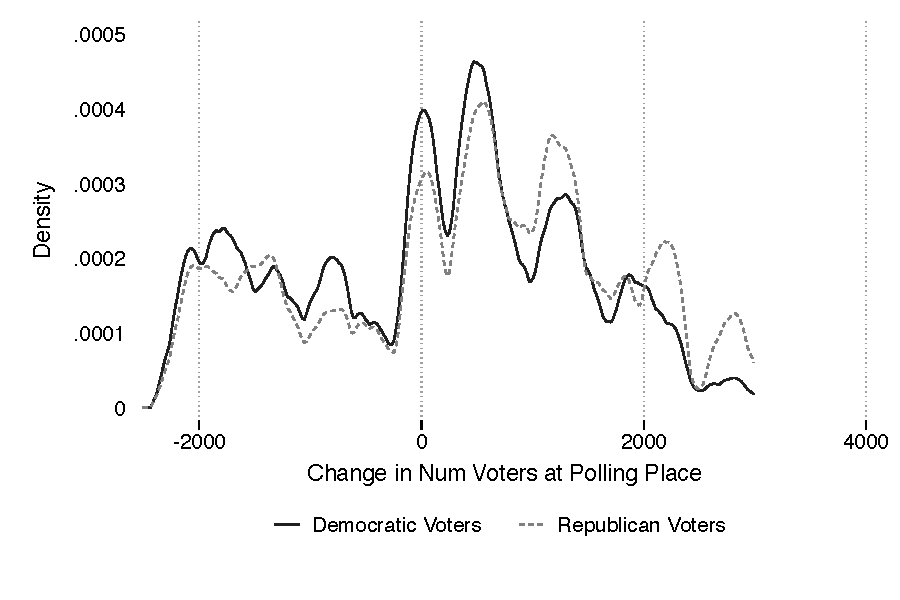
\includegraphics{../../50_results_full/kdensity_change_pp_registrants.pdf}
		\end{center}
\end{figure} \normalsize


%% FIGURE
%%-------
\begin{figure}[h!]
	\begin{center}
	\caption{Distribution of Changes in the Number of Polling Place Registrants Voter Party Registration and Year} \label{KDPPbyPartybyYear}
		\small \vspace*{.08in}
    (a) Democrat-appointed (2012) \hspace*{1.2in} (b) Republican-appointed (2016) \\
		\smallskip
		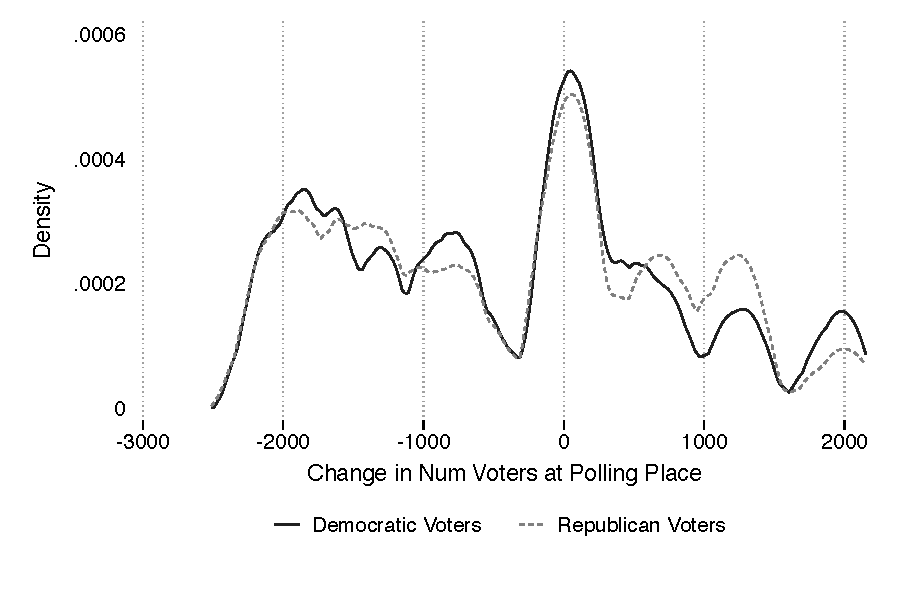
\includegraphics[width=0.48\textwidth]{../../50_results_full/kdensity_change_pp_registrants_2012.pdf}		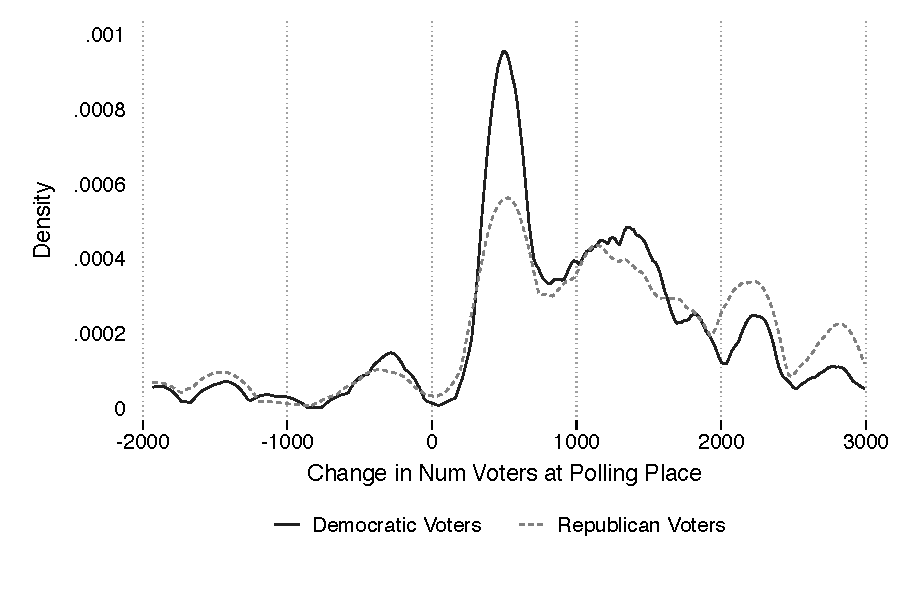
\includegraphics[width=0.48\textwidth]{../../50_results_full/kdensity_change_pp_registrants_2016.pdf}
		\end{center}
\end{figure} \normalsize


Figure \ref{KDPPbyPartybyYear} replicates Figure \ref{KDPPbyParty} to separately characterize the impact of changes made in 2012 by Democrats and the changes made in 2016 by Republicans.  The left hand plot reveals that Democrats were far more likely than Republicans to decrease the number of voters per polling place (as is evidenced by the fact that the density is often higher for values less than 0). In contrast, the allocations made by Republicans almost uniformly increase the number of people per polling place and very few voters experience a decrease in the number of voters per polling place.

Despite these differences, it is also clear that the patterns do not vary by the partisanship of affected voters.  Although Democrats appear more likely to decrease the number of voters per polling place than Republicans, Democrats and Republicans appear to be similarly impacted. Likewise both Democrats and Republicans have more voters added to their precinct in 2016 by Republican administrators. Thus, while there are differences in the nature of the relationship depending on the party in charge, there is not evidence that those differences have disparate consequences on voters.


%------------------------------------ APPENDIX E: Full Specifications ------------------------------------------%
\clearpage \newpage
\subsection{Normality of County-Level Point Estimates}\label{appendix_county_point_estimate_distributions}
\setcounter{table}{0}
\setcounter{figure}{0}
\renewcommand{\thetable}{E\arabic{table}}
\renewcommand{\thefigure}{E\arabic{figure}}

In this appendix we present additional evidence that the variation in the county-level coefficients that we estimate are due to random voter-level shocks rather than heterogeneity in the willingness and capacity of local administrators to strategically manipulate polling places.


\begin{figure}[h!]
	\begin{center}
	\caption{Normality of County-Level Estimates of Targeting (P-P Plot)}\label{figure_normalitytests_pp}
		\small \vspace*{.05in}
		\smallskip

    (a) Democrat-appointed (2012)\\
		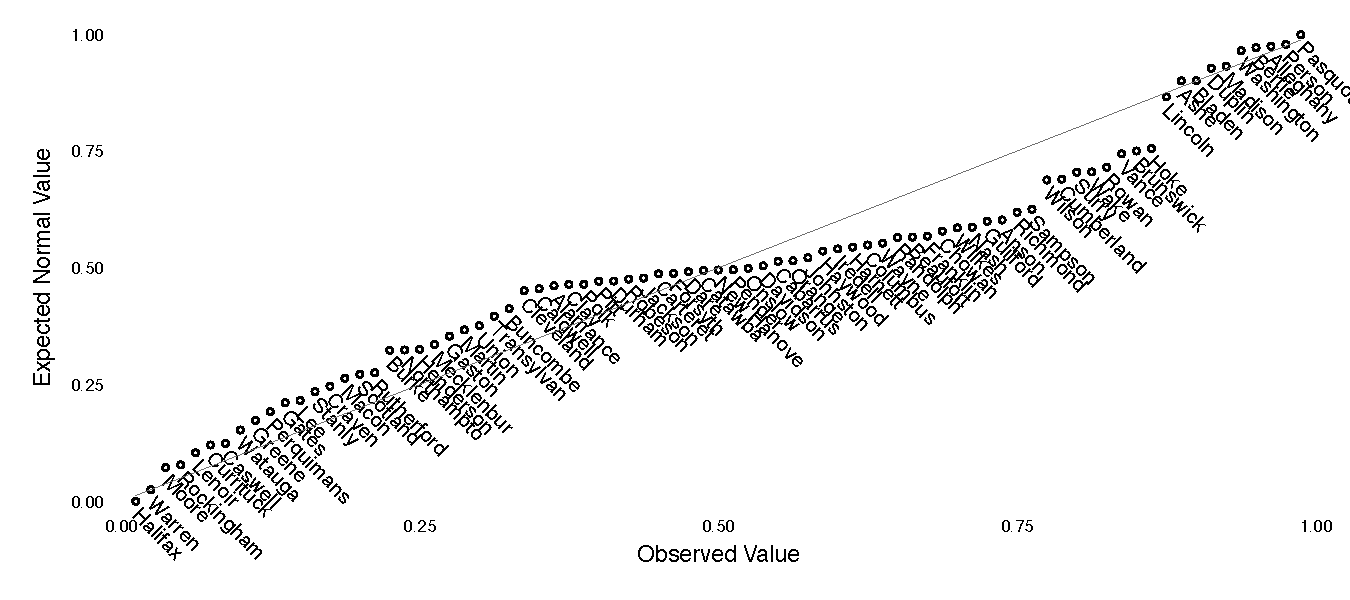
\includegraphics[width=6.2in]{../../50_results_full/county_point_estimate_pnorm_pp_has_changed_2012.pdf}  \\

    \smallskip
    (b) Republican-appointed (2016)\\
    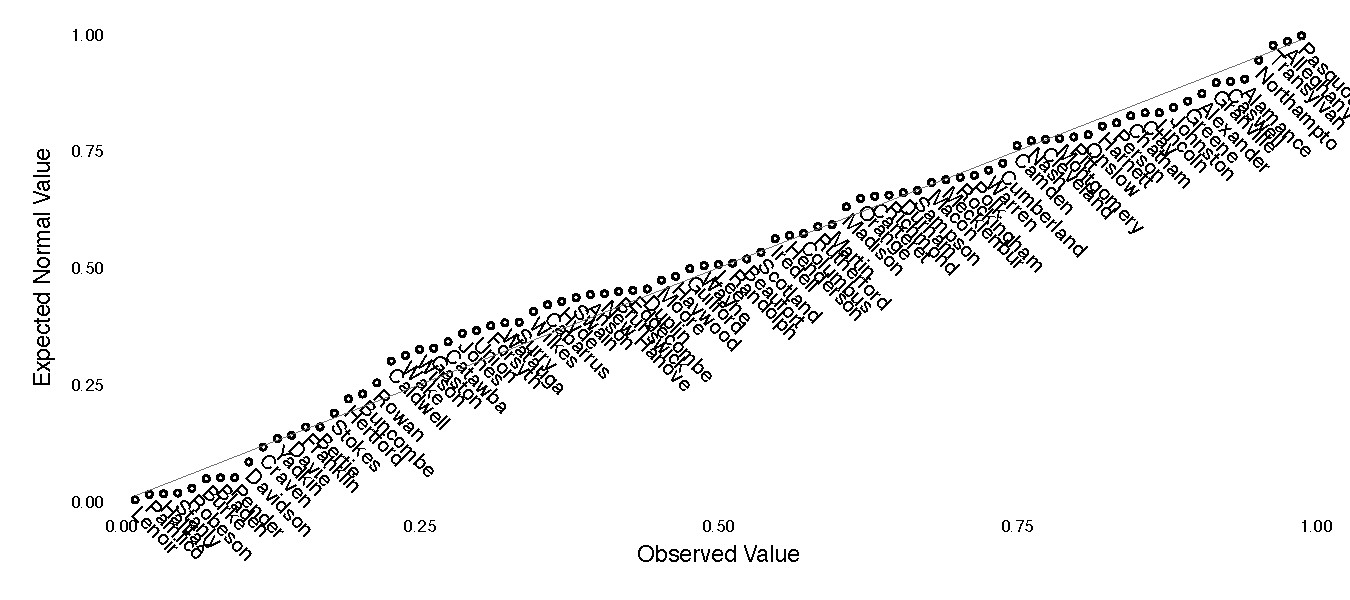
\includegraphics[width=6.2in]{../../50_results_full/county_point_estimate_pnorm_pp_has_changed_2016.pdf}

		\end{center}
\end{figure} \normalsize

Figure \ref{figure_normalitytests_pp} plots the distribution of county-specific effects against the percentiles of the normal distribution.  If the results were normal, the estimates should align the 45-degree line.  While some counties appear to be slightly less likely to experience a change than might be expected if a random process were responsible for making the changes, the impacted counties are not obviously high-Democrat counties and most of the estimated effects nearly match the effects predicted by the percentiles of the normal distribution.  The effects for Republican-led changes are even more consistent with the assumption of effects produced randomly from the normal distribution.





%% --------------------------------------- APPENDIX: County Targeting Estimates  --------------------------------------- %%
\clearpage \newpage
\subsection{County Targeting Estimates and County Demographics}\label{appendix_countytargetinganddemographics}
\setcounter{table}{0}
\setcounter{figure}{0}
\renewcommand{\thetable}{F\arabic{table}}
\renewcommand{\thefigure}{F\arabic{figure}}

In this appendix we demonstrate that there is no relationship between county characteristics and our county-level estimate of differential polling place changes by partisanship.  Each plot in Figure~\ref{figure_county_demographics} presents the scatter plot of our estimates of opposition targeting ($\hat{\beta}$) from estimating equation~\ref{equation_panel_party} and their relationship to Democratic party vote share in the county (plots (a) and (b)), and the share of the county that is black (plots (c) and (d)). In addition, we also test for whether targeting is more likely in divided counties (where the incentive to target to improve outcomes in local races may be higher) (plots (e) and (f), where \emph{Swing County} is defined as $1 - abs(vote share - 0.5)$, and takes on value of 1 when a county has a 50-50 party split, 0 if 100\% one party).  In all of the plots, there is no relationship between our estimates and county characteristics.  This evidence supports our claim that local officials did not choose a county-level strategy of targeting that focused explicitly on more Democratic or more minority counties.

\begin{figure}[h!]
	\begin{center}
    \label{figure_county_demographics}
	\caption{County Targeting Estimates and Demographics}
  \vspace{.1in} \small
    (a) Democratic Vote Share, 2012 \hspace*{.8in} (b) Democratic Vote Share, 2016 \\
		    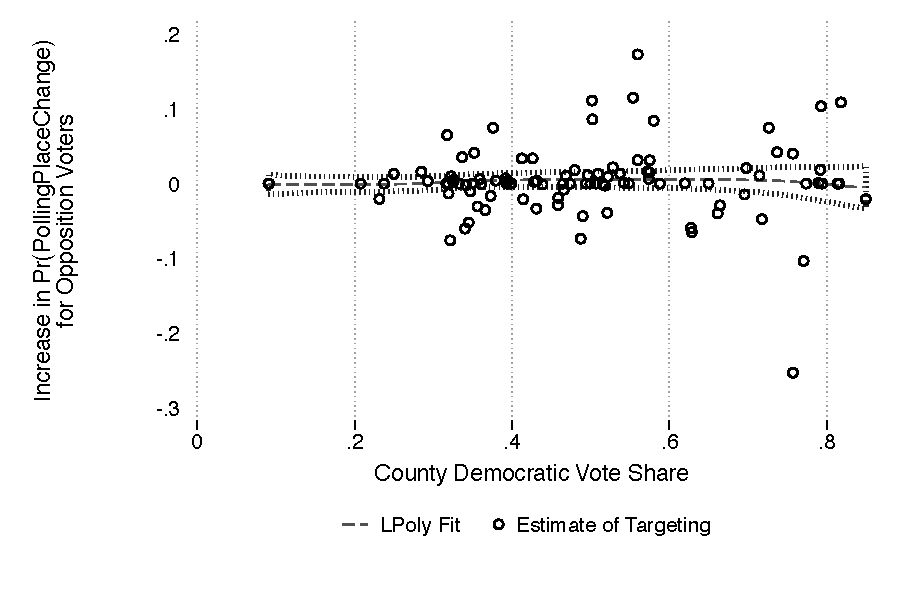
\includegraphics[width=0.4\textwidth]{../../50_results_full/countyestimates_party_dem_2012.pdf}
        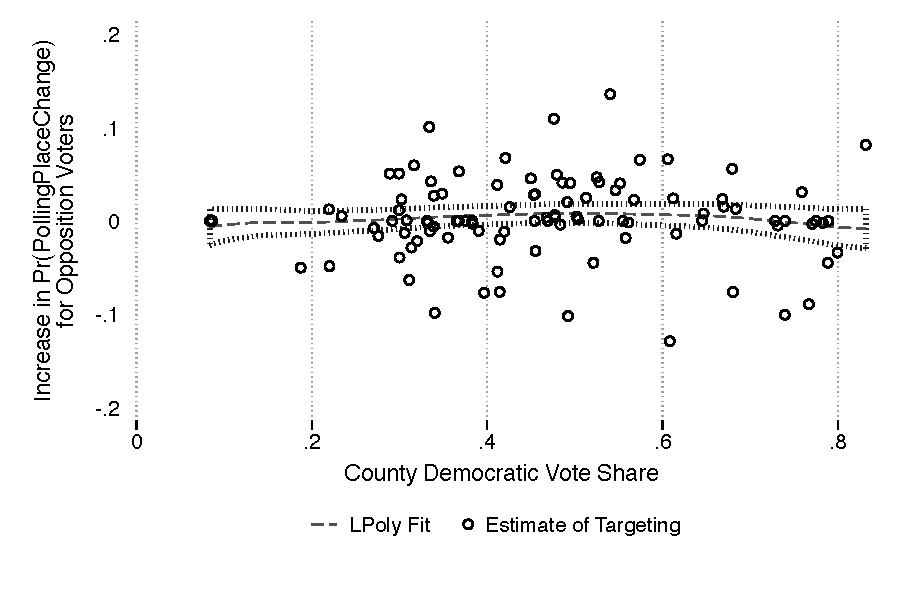
\includegraphics[width=0.4\textwidth]{../../50_results_full/countyestimates_party_dem_2016.pdf}\\
        \smallskip
        (c) Share Black, 2012 \hspace*{1.5in} (d) Share Black, 2016 \\
        \smallskip
        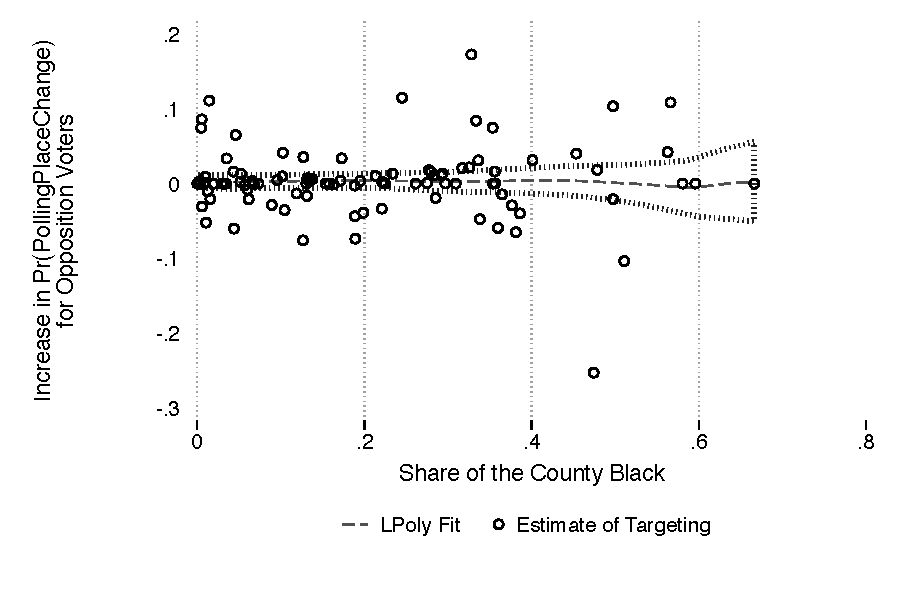
\includegraphics[width=0.4\textwidth]{../../50_results_full/countyestimates_race_black_2012.pdf} 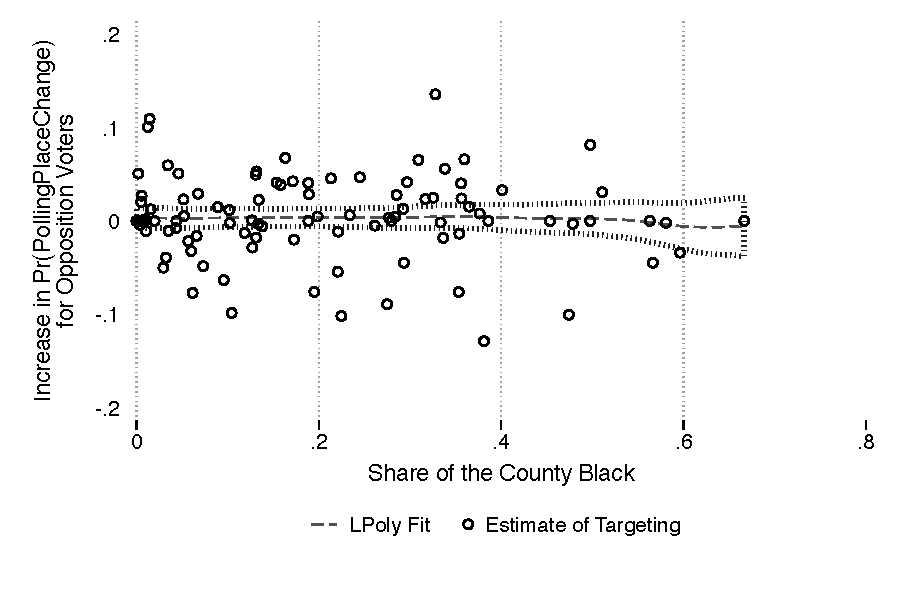
\includegraphics[width=0.4\textwidth]{../../50_results_full/countyestimates_race_black_2016.pdf} \\
		\smallskip
		(e) Swing County, 2012 \hspace*{1.5in} (f) Swing County, 2016 \\
		\smallskip
        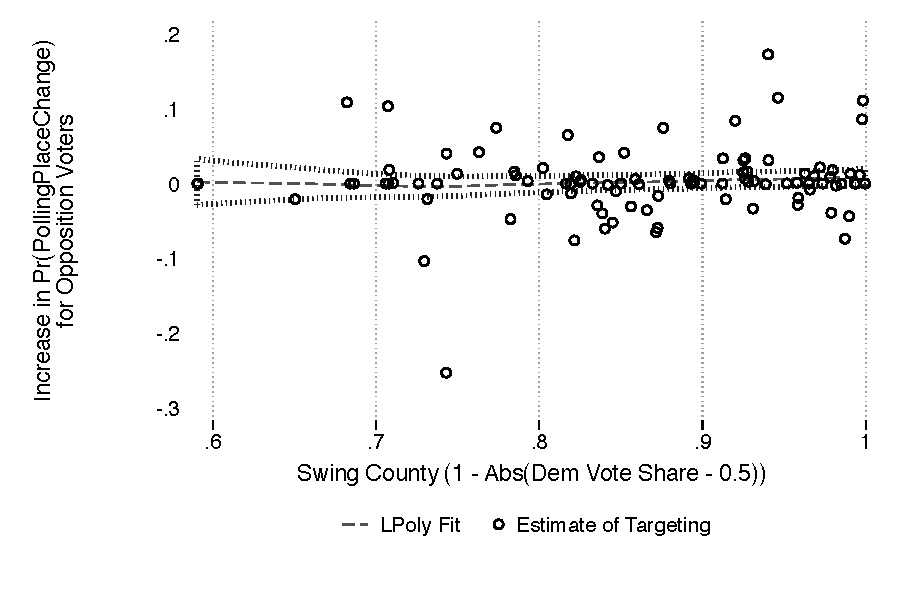
\includegraphics[width=0.4\textwidth]{../../50_results_full/countyestimates_swing_county_2012.pdf} 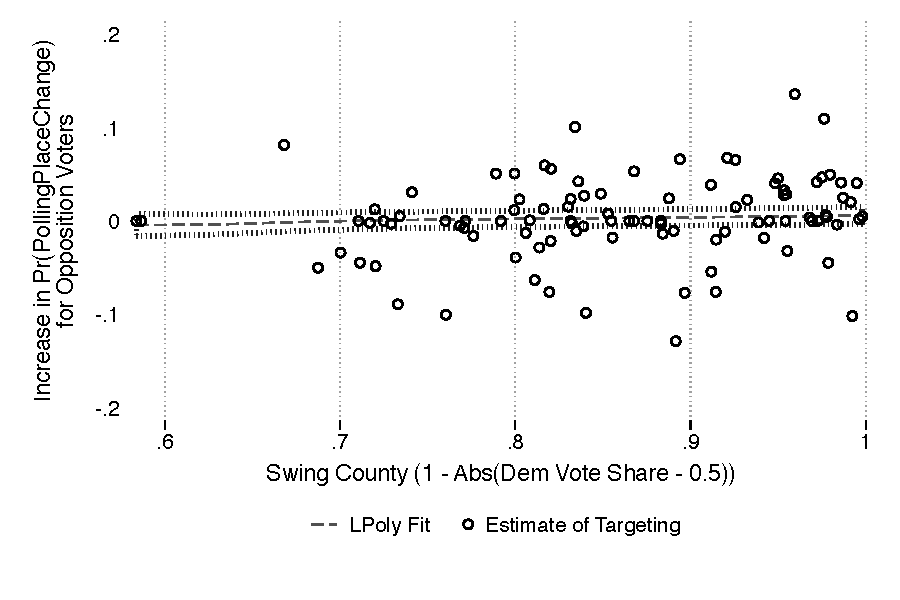
\includegraphics[width=0.4\textwidth]{../../50_results_full/countyestimates_swing_county_2016.pdf}
		\end{center}
\end{figure} \normalsize



%% --------------------------------------- APPENDIX: Responsive Counties --------------------------------------- %%
\clearpage \newpage
\subsection{ Subsetting on Political Responsive Counties}\label{appendix_politically_responsive_counties}
\setcounter{table}{0}
\setcounter{figure}{0}
\renewcommand{\thetable}{G\arabic{table}}
\renewcommand{\thefigure}{G\arabic{figure}}

Following the Republican election in 2012, journalists obtained emails from the executive director of the North Carolina Republican Party reminding Republican county board members and other party officials that ``our Republican Board members should feel empowered to make legal changes to early voting plans, that are supported by Republicans\ldots Republicans can and should make party line changes to early voting'' \citep{campbell2016c}. Subsequent reporting found that ten counties followed the suggestion of Republican leaders to reduce Sunday early voting hours and locations---Craven, Cumberland, Edgecombe, Forsyth, Hoke, Pamlico, Pitt, Richmond, Union, and Lenoir \citep{campbell2016c}. Other reporting found several counties engaged in a series of precinct consolidations that seemed to be consistent with politically-motivated targeting---Cleveland, Pasquotank, Beaufort, Caswell, Halifax, Martin, Nash, Person, Robeson, and Wayne Counties \citep{ncprecincts}. As this suggests these counties may be particularly susceptible to partisan direction, we subset our analyses to just these counties to test whether, at least in these ostensibly partisan counties, we can detect effects of targeting.

Table~\ref{table_responsive} repeats our main analysis restricted to this subset of twenty politically-responsive counties. If the systematic use of polling place changes is being used to target voters anywhere in North Carolina, these counties seem like the most-likely places for us to observe such targeting.  Given that Republican-appointees controlled county election boards during this period, $Opposition$ measures Democratic voters.  As Table~\ref{table_responsive} shows, however, we again find no evidence of systematic targeting of voters.  While our estimates may be indistinguishable from zero as a consequence of our small number of county clusters, the magnitude of our estimates is consistently small, even at the upper bound of the 95\% confidence interval.  Our estimates of the coefficient on $Opposition$ for \emph{per se} polling place changes and distance (models 1 and 3) are less than half of a percentage point in magnitude.  And the differential effect for Black Democrats is similarly exceptionally small.  Even the upper bound of the 95\% confidence interval suggests that, at most, precincts used by Democrats  saw consolidation that resulted in only $\sim$15\% of a standard deviation more voters at a polling place.


%% TABLE: Politically Responsive Counties
%%---------------------------------------
 \begin{table}[t!]\centering \footnotesize
 \def\sym#1{\ifmmode^{#1}\else\(^{#1}\)\fi}
 	\caption{Republican Precinct and Polling Place Changes in Politically Responsive Counties, 2016}\label{table_responsive}
 	\smallskip
 	\begin{tabular}{@{\extracolsep{5pt}}l*{6}{c}}
 	\noalign{\smallskip}\hline\hline\noalign{\smallskip}\noalign{\smallskip}
    &  \multicolumn{2}{c}{$Pr(\Delta PollingPlace)$} & \multicolumn{2}{c}{$Pr(PP Moved Farther)$} & \multicolumn{2}{c}{$\Delta VotersPerPrecinct$}   \\
    \cline{2-3} \cline{4-5} \cline{6-7} \noalign{\smallskip}
 				                &\multicolumn{1}{c}{(1)}         &\multicolumn{1}{c}{(2)}         &\multicolumn{1}{c}{(3)}         &\multicolumn{1}{c}{(4)}         &\multicolumn{1}{c}{(5)}         &\multicolumn{1}{c}{(6)}         \\
\midrule
\emph{Opposition}& -0.00087         &                  &   0.0020         &                  &    -1.62         &                  \\
                & (0.0099)         &                  &  (0.028)         &                  &   (11.7)         &                  \\
\emph{WhiteOpposition}&                  &  -0.0011         &                  &    0.012         &                  &    -2.91         \\
                &                  & (0.0046)         &                  &  (0.012)         &                  &   (6.04)         \\
\emph{BlackOpposition}&                  &   0.0017         &                  &  -0.0075         &                  &     1.42         \\
                &                  &  (0.018)         &                  &  (0.048)         &                  &   (18.0)         \\
\midrule
Controls        &\checkmark         &\checkmark         &\checkmark         &\checkmark         &\checkmark         &\checkmark         \\
County FE       &\checkmark         &\checkmark         &\checkmark         &\checkmark         &\checkmark         &\checkmark         \\
Observations    &   447793         &   447793         &    78801         &    78801         &   447749         &   447749         \\
Mean of DV      &     0.18         &     0.18         &     0.59         &     0.59         &     71.3         &     71.3         \\
SD of DV        &     0.35         &     0.35         &     0.45         &     0.45         &    286.8         &    286.8         \\
County Clusters &       20         &       20         &       19         &       19         &       20         &       20         \\
 \\
 	\noalign{\vspace*{-.17in}}\hline\hline\noalign{\smallskip}
 \multicolumn{7}{p{4.0in}}{\scriptsize Standard errors clustered at the county level. } \\
 \multicolumn{7}{l}{\scriptsize \sym{*} \(p<0.1\), \sym{**} \(p<0.05\), \sym{***} \(p<0.01\)}\\
 \multicolumn{7}{p{5.6in}}{\scriptsize  \emph{Notes:} The table presents coefficients from estimating Equation~\ref{equation_panel_party} (columns 1, 3, 5) and Equation~\ref{equation_panel_partyrace} (columns 2, 4, 6) using OLS restricted to the twenty politically-responsive counties identified in the text in 2016 under Republican control.  The unit of analysis is the voter. Our controls are linear and quadratic $Age$. Estimates of targeting for $Pr(PPMovedFurther)$ are conditional on experiencing a polling place change, accounting for the different sample sizes. See Appendix~\ref{appendix_maintargeting} for the full set of coefficient estimates including those for unaffiliated voters. }
 \end{tabular}
 \end{table}



%% --------------------------------------- APPENDIX: Shelby v. Holder --------------------------------------- %%
\clearpage \newpage
\subsection{ Additional \emph{Shelby v. Holder} Graphical Evidence}\label{appendix_shelby}
\setcounter{table}{0}
\setcounter{figure}{0}
\renewcommand{\thetable}{H\arabic{table}}
\renewcommand{\thefigure}{H\arabic{figure}}


In this appendix we present additional graphical evidence related to the relationship between precinct and polling place changes and coverage under Section 5 of the VRA.


\begin{figure}[h!]
	\begin{center}
    \label{figure_shelby_distribution}
	\caption{Distribution of County-Level Estimates of Polling Place Changes by Section 5 Coverage, 2016}
          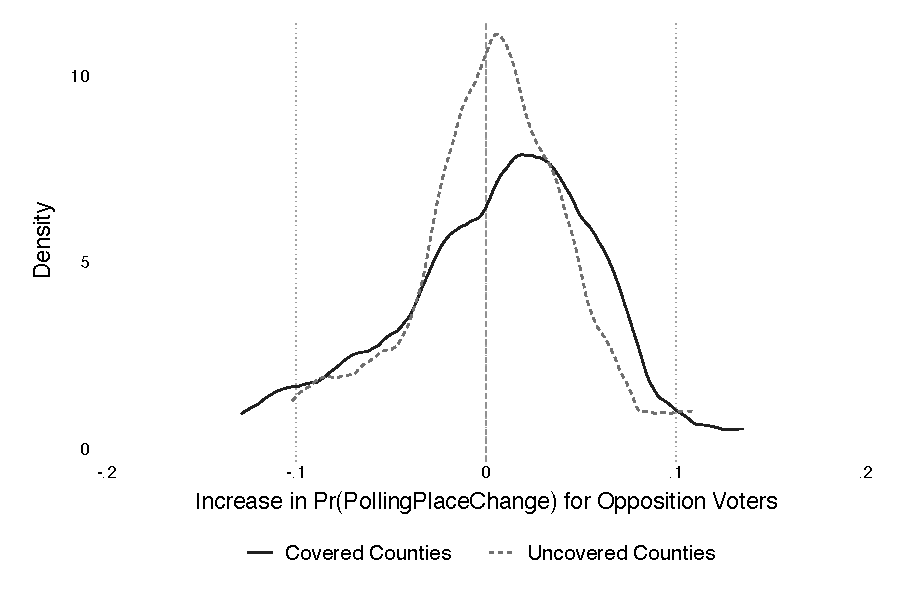
\includegraphics[width=0.65\textwidth]{../../50_results_full/county_point_estimate_density_vra.pdf}\\
        \end{center}
    \end{figure} \normalsize


Figure~\ref{figure_shelby_distribution} plots the distribution of county-level point estimates of the effect of a polling place change for opposition voters.  There are not meaningful differences in the distributions, suggesting that the average differences that we present and discuss in the text of the main paper do not hide important variation in the effects that might be consistent with local election administrators responding to the removal of Section 5 coverage.

Figure~\ref{figure_shelby_dind} presents raw trends in the probability of an opposition voter experiencing a polling place change by coverage status.  The vertical line indicates the year of the \emph{Shelby} decision.  The average probability of an opposition voter experiencing a polling place change declined by more in uncovered counties than covered counties.  Were we to think that the uncovered counties represented the appropriate counterfactual for covered counties, then this might suggest evidence of differential targeting based on Shelby (although we emphasize that this is the raw data and a regression would account for county fixed effects and other covariates).  For reasons discussed in the text, however, we still don't find convincing the argument that trends in uncovered counties are an appropriate counterfactual.


    \begin{figure}[h!]
    	\begin{center}
        \label{figure_shelby_dind}
    	\caption{Trends in Mean Probability of an Opposition Voter Experiencing a Polling Place Change by Section 5 Coverage}
              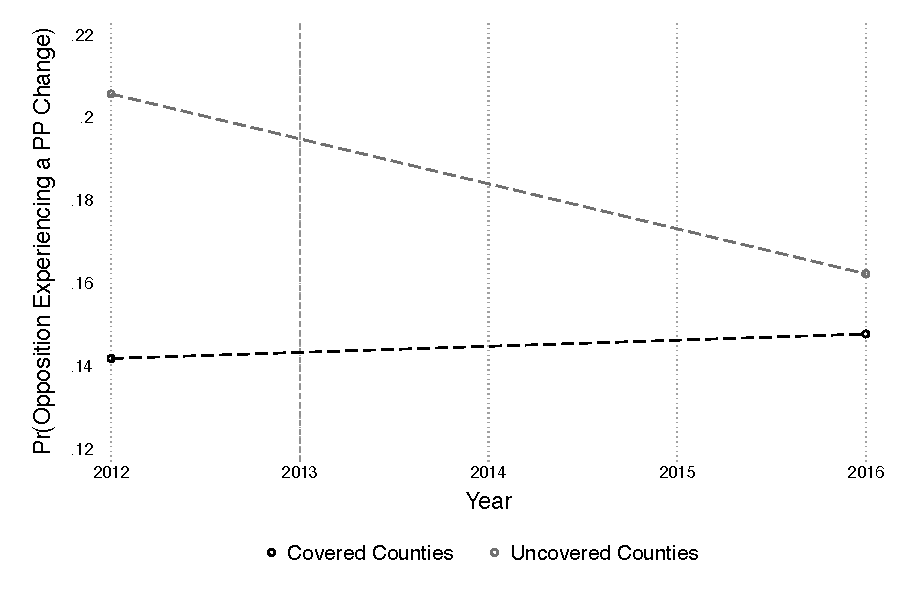
\includegraphics[width=0.65\textwidth]{../../50_results_full/shelby_dind.pdf}\\
            \end{center}
        \end{figure} \normalsize



%--------------------------------------------- END OF DOCUMENT ------------------------------------------------%

\end{document}
